\documentclass[twoside]{book}

% Packages required by doxygen
\usepackage{fixltx2e}
\usepackage{calc}
\usepackage{doxygen}
\usepackage[export]{adjustbox} % also loads graphicx
\usepackage{graphicx}
\usepackage[utf8]{inputenc}
\usepackage{makeidx}
\usepackage{multicol}
\usepackage{multirow}
\PassOptionsToPackage{warn}{textcomp}
\usepackage{textcomp}
\usepackage[nointegrals]{wasysym}
\usepackage[table]{xcolor}

% Font selection
\usepackage[T1]{fontenc}
\usepackage[scaled=.90]{helvet}
\usepackage{courier}
\usepackage{amssymb}
\usepackage{sectsty}
\renewcommand{\familydefault}{\sfdefault}
\allsectionsfont{%
  \fontseries{bc}\selectfont%
  \color{darkgray}%
}
\renewcommand{\DoxyLabelFont}{%
  \fontseries{bc}\selectfont%
  \color{darkgray}%
}
\newcommand{\+}{\discretionary{\mbox{\scriptsize$\hookleftarrow$}}{}{}}

% Page & text layout
\usepackage{geometry}
\geometry{%
  a4paper,%
  top=2.5cm,%
  bottom=2.5cm,%
  left=2.5cm,%
  right=2.5cm%
}
\tolerance=750
\hfuzz=15pt
\hbadness=750
\setlength{\emergencystretch}{15pt}
\setlength{\parindent}{0cm}
\setlength{\parskip}{3ex plus 2ex minus 2ex}
\makeatletter
\renewcommand{\paragraph}{%
  \@startsection{paragraph}{4}{0ex}{-1.0ex}{1.0ex}{%
    \normalfont\normalsize\bfseries\SS@parafont%
  }%
}
\renewcommand{\subparagraph}{%
  \@startsection{subparagraph}{5}{0ex}{-1.0ex}{1.0ex}{%
    \normalfont\normalsize\bfseries\SS@subparafont%
  }%
}
\makeatother

% Headers & footers
\usepackage{fancyhdr}
\pagestyle{fancyplain}
\fancyhead[LE]{\fancyplain{}{\bfseries\thepage}}
\fancyhead[CE]{\fancyplain{}{}}
\fancyhead[RE]{\fancyplain{}{\bfseries\leftmark}}
\fancyhead[LO]{\fancyplain{}{\bfseries\rightmark}}
\fancyhead[CO]{\fancyplain{}{}}
\fancyhead[RO]{\fancyplain{}{\bfseries\thepage}}
\fancyfoot[LE]{\fancyplain{}{}}
\fancyfoot[CE]{\fancyplain{}{}}
\fancyfoot[RE]{\fancyplain{}{\bfseries\scriptsize Generated by Doxygen }}
\fancyfoot[LO]{\fancyplain{}{\bfseries\scriptsize Generated by Doxygen }}
\fancyfoot[CO]{\fancyplain{}{}}
\fancyfoot[RO]{\fancyplain{}{}}
\renewcommand{\footrulewidth}{0.4pt}
\renewcommand{\chaptermark}[1]{%
  \markboth{#1}{}%
}
\renewcommand{\sectionmark}[1]{%
  \markright{\thesection\ #1}%
}

% Indices & bibliography
\usepackage{natbib}
\usepackage[titles]{tocloft}
\setcounter{tocdepth}{3}
\setcounter{secnumdepth}{5}
\makeindex

% Hyperlinks (required, but should be loaded last)
\usepackage{ifpdf}
\ifpdf
  \usepackage[pdftex,pagebackref=true]{hyperref}
\else
  \usepackage[ps2pdf,pagebackref=true]{hyperref}
\fi
\hypersetup{%
  colorlinks=true,%
  linkcolor=blue,%
  citecolor=blue,%
  unicode%
}

% Custom commands
\newcommand{\clearemptydoublepage}{%
  \newpage{\pagestyle{empty}\cleardoublepage}%
}

\usepackage{caption}
\captionsetup{labelsep=space,justification=centering,font={bf},singlelinecheck=off,skip=4pt,position=top}

%===== C O N T E N T S =====

\begin{document}

% Titlepage & ToC
\hypersetup{pageanchor=false,
             bookmarksnumbered=true,
             pdfencoding=unicode
            }
\pagenumbering{roman}
\begin{titlepage}
\vspace*{7cm}
\begin{center}%
{\Large Virtual Zoo V\+Z03 }\\
\vspace*{1cm}
{\large Generated by Doxygen 1.8.11}\\
\end{center}
\end{titlepage}
\clearemptydoublepage
\tableofcontents
\clearemptydoublepage
\pagenumbering{arabic}
\hypersetup{pageanchor=true}

%--- Begin generated contents ---
\chapter{Hierarchical Index}
\section{Class Hierarchy}
This inheritance list is sorted roughly, but not completely, alphabetically\+:\begin{DoxyCompactList}
\item \contentsline{section}{Animal}{\pageref{class_animal}}{}
\begin{DoxyCompactList}
\item \contentsline{section}{Air\+Animal}{\pageref{class_air_animal}}{}
\begin{DoxyCompactList}
\item \contentsline{section}{Accipitridae}{\pageref{class_accipitridae}}{}
\begin{DoxyCompactList}
\item \contentsline{section}{Eagle}{\pageref{class_eagle}}{}
\end{DoxyCompactList}
\item \contentsline{section}{Passeridae}{\pageref{class_passeridae}}{}
\begin{DoxyCompactList}
\item \contentsline{section}{Burung\+Gereja}{\pageref{class_burung_gereja}}{}
\end{DoxyCompactList}
\item \contentsline{section}{Phasianidae}{\pageref{class_phasianidae}}{}
\begin{DoxyCompactList}
\item \contentsline{section}{Merak}{\pageref{class_merak}}{}
\item \contentsline{section}{Pegar}{\pageref{class_pegar}}{}
\end{DoxyCompactList}
\item \contentsline{section}{Psittacifurmes}{\pageref{class_psittacifurmes}}{}
\begin{DoxyCompactList}
\item \contentsline{section}{Beo\+Nias}{\pageref{class_beo_nias}}{}
\item \contentsline{section}{Kakatua}{\pageref{class_kakatua}}{}
\end{DoxyCompactList}
\end{DoxyCompactList}
\item \contentsline{section}{Herbivora}{\pageref{class_herbivora}}{}
\begin{DoxyCompactList}
\item \contentsline{section}{African\+Elephant}{\pageref{class_african_elephant}}{}
\item \contentsline{section}{Anoa}{\pageref{class_anoa}}{}
\item \contentsline{section}{Beo\+Nias}{\pageref{class_beo_nias}}{}
\item \contentsline{section}{Burung\+Gereja}{\pageref{class_burung_gereja}}{}
\item \contentsline{section}{Chimpanzee}{\pageref{class_chimpanzee}}{}
\item \contentsline{section}{Donkey}{\pageref{class_donkey}}{}
\item \contentsline{section}{Girrafe}{\pageref{class_girrafe}}{}
\item \contentsline{section}{Goat}{\pageref{class_goat}}{}
\item \contentsline{section}{Gorilla}{\pageref{class_gorilla}}{}
\item \contentsline{section}{Horse}{\pageref{class_horse}}{}
\item \contentsline{section}{Kakatua}{\pageref{class_kakatua}}{}
\item \contentsline{section}{Moose}{\pageref{class_moose}}{}
\item \contentsline{section}{Okapi}{\pageref{class_okapi}}{}
\item \contentsline{section}{Orangutan}{\pageref{class_orangutan}}{}
\item \contentsline{section}{Panda}{\pageref{class_panda}}{}
\item \contentsline{section}{Reindeer}{\pageref{class_reindeer}}{}
\item \contentsline{section}{Rhino}{\pageref{class_rhino}}{}
\item \contentsline{section}{Sheep}{\pageref{class_sheep}}{}
\item \contentsline{section}{Squirrel\+Monkey}{\pageref{class_squirrel_monkey}}{}
\item \contentsline{section}{Sumatra\+Elephant}{\pageref{class_sumatra_elephant}}{}
\item \contentsline{section}{Zebra}{\pageref{class_zebra}}{}
\end{DoxyCompactList}
\item \contentsline{section}{Karnivora}{\pageref{class_karnivora}}{}
\begin{DoxyCompactList}
\item \contentsline{section}{Cape\+Cobra}{\pageref{class_cape_cobra}}{}
\item \contentsline{section}{Carpet\+Python}{\pageref{class_carpet_python}}{}
\item \contentsline{section}{Cat}{\pageref{class_cat}}{}
\item \contentsline{section}{Crocodile}{\pageref{class_crocodile}}{}
\item \contentsline{section}{Dog}{\pageref{class_dog}}{}
\item \contentsline{section}{Dolphin}{\pageref{class_dolphin}}{}
\item \contentsline{section}{Eagle}{\pageref{class_eagle}}{}
\item \contentsline{section}{Fox}{\pageref{class_fox}}{}
\item \contentsline{section}{Hammer\+Shark}{\pageref{class_hammer_shark}}{}
\item \contentsline{section}{Hyena}{\pageref{class_hyena}}{}
\item \contentsline{section}{Indian\+Python}{\pageref{class_indian_python}}{}
\item \contentsline{section}{King\+Cobra}{\pageref{class_king_cobra}}{}
\item \contentsline{section}{Lion}{\pageref{class_lion}}{}
\item \contentsline{section}{Mamba}{\pageref{class_mamba}}{}
\item \contentsline{section}{Panther}{\pageref{class_panther}}{}
\item \contentsline{section}{Penguin}{\pageref{class_penguin}}{}
\item \contentsline{section}{Salamander}{\pageref{class_salamander}}{}
\item \contentsline{section}{Sea\+Dragon}{\pageref{class_sea_dragon}}{}
\item \contentsline{section}{Sea\+Horse}{\pageref{class_sea_horse}}{}
\item \contentsline{section}{Tiger}{\pageref{class_tiger}}{}
\item \contentsline{section}{Tiger\+Snake}{\pageref{class_tiger_snake}}{}
\item \contentsline{section}{Tree\+Frog}{\pageref{class_tree_frog}}{}
\item \contentsline{section}{Whale}{\pageref{class_whale}}{}
\item \contentsline{section}{White\+Shark}{\pageref{class_white_shark}}{}
\item \contentsline{section}{Wolf}{\pageref{class_wolf}}{}
\end{DoxyCompactList}
\item \contentsline{section}{Land\+Animal}{\pageref{class_land_animal}}{}
\begin{DoxyCompactList}
\item \contentsline{section}{Bovidae}{\pageref{class_bovidae}}{}
\begin{DoxyCompactList}
\item \contentsline{section}{Anoa}{\pageref{class_anoa}}{}
\item \contentsline{section}{Goat}{\pageref{class_goat}}{}
\item \contentsline{section}{Sheep}{\pageref{class_sheep}}{}
\end{DoxyCompactList}
\item \contentsline{section}{Canidae}{\pageref{class_canidae}}{}
\begin{DoxyCompactList}
\item \contentsline{section}{Dog}{\pageref{class_dog}}{}
\item \contentsline{section}{Fox}{\pageref{class_fox}}{}
\item \contentsline{section}{Wolf}{\pageref{class_wolf}}{}
\end{DoxyCompactList}
\item \contentsline{section}{Cercopithecidae}{\pageref{class_cercopithecidae}}{}
\begin{DoxyCompactList}
\item \contentsline{section}{Squirrel\+Monkey}{\pageref{class_squirrel_monkey}}{}
\end{DoxyCompactList}
\item \contentsline{section}{Cervidae}{\pageref{class_cervidae}}{}
\begin{DoxyCompactList}
\item \contentsline{section}{Moose}{\pageref{class_moose}}{}
\item \contentsline{section}{Reindeer}{\pageref{class_reindeer}}{}
\end{DoxyCompactList}
\item \contentsline{section}{Crocodylidae}{\pageref{class_crocodylidae}}{}
\begin{DoxyCompactList}
\item \contentsline{section}{Crocodile}{\pageref{class_crocodile}}{}
\end{DoxyCompactList}
\item \contentsline{section}{Cryptobranchidae}{\pageref{class_cryptobranchidae}}{}
\begin{DoxyCompactList}
\item \contentsline{section}{Salamander}{\pageref{class_salamander}}{}
\end{DoxyCompactList}
\item \contentsline{section}{Elapidae}{\pageref{class_elapidae}}{}
\begin{DoxyCompactList}
\item \contentsline{section}{Cape\+Cobra}{\pageref{class_cape_cobra}}{}
\item \contentsline{section}{King\+Cobra}{\pageref{class_king_cobra}}{}
\item \contentsline{section}{Mamba}{\pageref{class_mamba}}{}
\item \contentsline{section}{Tiger\+Snake}{\pageref{class_tiger_snake}}{}
\end{DoxyCompactList}
\item \contentsline{section}{Elephantidae}{\pageref{class_elephantidae}}{}
\begin{DoxyCompactList}
\item \contentsline{section}{African\+Elephant}{\pageref{class_african_elephant}}{}
\item \contentsline{section}{Sumatra\+Elephant}{\pageref{class_sumatra_elephant}}{}
\end{DoxyCompactList}
\item \contentsline{section}{Equidae}{\pageref{class_equidae}}{}
\begin{DoxyCompactList}
\item \contentsline{section}{Donkey}{\pageref{class_donkey}}{}
\item \contentsline{section}{Horse}{\pageref{class_horse}}{}
\item \contentsline{section}{Zebra}{\pageref{class_zebra}}{}
\end{DoxyCompactList}
\item \contentsline{section}{Felidae}{\pageref{class_felidae}}{}
\begin{DoxyCompactList}
\item \contentsline{section}{Cat}{\pageref{class_cat}}{}
\item \contentsline{section}{Lion}{\pageref{class_lion}}{}
\item \contentsline{section}{Panther}{\pageref{class_panther}}{}
\item \contentsline{section}{Tiger}{\pageref{class_tiger}}{}
\end{DoxyCompactList}
\item \contentsline{section}{Girrafidae}{\pageref{class_girrafidae}}{}
\begin{DoxyCompactList}
\item \contentsline{section}{Girrafe}{\pageref{class_girrafe}}{}
\item \contentsline{section}{Okapi}{\pageref{class_okapi}}{}
\end{DoxyCompactList}
\item \contentsline{section}{Hominidae}{\pageref{class_hominidae}}{}
\begin{DoxyCompactList}
\item \contentsline{section}{Chimpanzee}{\pageref{class_chimpanzee}}{}
\item \contentsline{section}{Gorilla}{\pageref{class_gorilla}}{}
\item \contentsline{section}{Orangutan}{\pageref{class_orangutan}}{}
\end{DoxyCompactList}
\item \contentsline{section}{Hyaenidae}{\pageref{class_hyaenidae}}{}
\begin{DoxyCompactList}
\item \contentsline{section}{Hyena}{\pageref{class_hyena}}{}
\end{DoxyCompactList}
\item \contentsline{section}{Hylidae}{\pageref{class_hylidae}}{}
\begin{DoxyCompactList}
\item \contentsline{section}{Tree\+Frog}{\pageref{class_tree_frog}}{}
\end{DoxyCompactList}
\item \contentsline{section}{Pythonidae}{\pageref{class_pythonidae}}{}
\begin{DoxyCompactList}
\item \contentsline{section}{Carpet\+Python}{\pageref{class_carpet_python}}{}
\item \contentsline{section}{Indian\+Python}{\pageref{class_indian_python}}{}
\end{DoxyCompactList}
\item \contentsline{section}{Rhinocerotidae}{\pageref{class_rhinocerotidae}}{}
\begin{DoxyCompactList}
\item \contentsline{section}{Rhino}{\pageref{class_rhino}}{}
\end{DoxyCompactList}
\item \contentsline{section}{Ursoidea}{\pageref{class_ursoidea}}{}
\begin{DoxyCompactList}
\item \contentsline{section}{Bear}{\pageref{class_bear}}{}
\item \contentsline{section}{Panda}{\pageref{class_panda}}{}
\end{DoxyCompactList}
\end{DoxyCompactList}
\item \contentsline{section}{Omnivora}{\pageref{class_omnivora}}{}
\begin{DoxyCompactList}
\item \contentsline{section}{Bear}{\pageref{class_bear}}{}
\item \contentsline{section}{Merak}{\pageref{class_merak}}{}
\item \contentsline{section}{Pari}{\pageref{class_pari}}{}
\item \contentsline{section}{Pegar}{\pageref{class_pegar}}{}
\end{DoxyCompactList}
\item \contentsline{section}{Water\+Animal}{\pageref{class_water_animal}}{}
\begin{DoxyCompactList}
\item \contentsline{section}{Cetacea}{\pageref{class_cetacea}}{}
\begin{DoxyCompactList}
\item \contentsline{section}{Dolphin}{\pageref{class_dolphin}}{}
\item \contentsline{section}{Whale}{\pageref{class_whale}}{}
\end{DoxyCompactList}
\item \contentsline{section}{Crocodylidae}{\pageref{class_crocodylidae}}{}
\item \contentsline{section}{Cryptobranchidae}{\pageref{class_cryptobranchidae}}{}
\item \contentsline{section}{Hylidae}{\pageref{class_hylidae}}{}
\item \contentsline{section}{Myliobatidae}{\pageref{class_myliobatidae}}{}
\begin{DoxyCompactList}
\item \contentsline{section}{Pari}{\pageref{class_pari}}{}
\end{DoxyCompactList}
\item \contentsline{section}{Selachimorpha}{\pageref{class_selachimorpha}}{}
\begin{DoxyCompactList}
\item \contentsline{section}{Hammer\+Shark}{\pageref{class_hammer_shark}}{}
\item \contentsline{section}{White\+Shark}{\pageref{class_white_shark}}{}
\end{DoxyCompactList}
\item \contentsline{section}{Spheniscidae}{\pageref{class_spheniscidae}}{}
\begin{DoxyCompactList}
\item \contentsline{section}{Penguin}{\pageref{class_penguin}}{}
\end{DoxyCompactList}
\item \contentsline{section}{Syngnathydae}{\pageref{class_syngnathydae}}{}
\begin{DoxyCompactList}
\item \contentsline{section}{Sea\+Dragon}{\pageref{class_sea_dragon}}{}
\item \contentsline{section}{Sea\+Horse}{\pageref{class_sea_horse}}{}
\end{DoxyCompactList}
\end{DoxyCompactList}
\end{DoxyCompactList}
\item \contentsline{section}{Cell}{\pageref{class_cell}}{}
\item \contentsline{section}{Renderable}{\pageref{class_renderable}}{}
\begin{DoxyCompactList}
\item \contentsline{section}{Cage}{\pageref{class_cage}}{}
\item \contentsline{section}{Point}{\pageref{class_point}}{}
\begin{DoxyCompactList}
\item \contentsline{section}{Facility}{\pageref{class_facility}}{}
\begin{DoxyCompactList}
\item \contentsline{section}{Park}{\pageref{class_park}}{}
\item \contentsline{section}{Restaurant}{\pageref{class_restaurant}}{}
\item \contentsline{section}{Road}{\pageref{class_road}}{}
\begin{DoxyCompactList}
\item \contentsline{section}{Entrance}{\pageref{class_entrance}}{}
\item \contentsline{section}{Exit}{\pageref{class_exit}}{}
\end{DoxyCompactList}
\end{DoxyCompactList}
\item \contentsline{section}{Habitat}{\pageref{class_habitat}}{}
\begin{DoxyCompactList}
\item \contentsline{section}{Air\+Habitat}{\pageref{class_air_habitat}}{}
\item \contentsline{section}{Land\+Habitat}{\pageref{class_land_habitat}}{}
\item \contentsline{section}{Water\+Habitat}{\pageref{class_water_habitat}}{}
\end{DoxyCompactList}
\end{DoxyCompactList}
\end{DoxyCompactList}
\end{DoxyCompactList}

\chapter{Class Index}
\section{Class List}
Here are the classes, structs, unions and interfaces with brief descriptions\+:\begin{DoxyCompactList}
\item\contentsline{section}{\hyperlink{class_african_elephant}{African\+Elephant} }{\pageref{class_african_elephant}}{}
\item\contentsline{section}{\hyperlink{class_african_elephant_test}{African\+Elephant\+Test} }{\pageref{class_african_elephant_test}}{}
\item\contentsline{section}{\hyperlink{class_air_habitat}{Air\+Habitat} }{\pageref{class_air_habitat}}{}
\item\contentsline{section}{\hyperlink{class_air_habitat_test}{Air\+Habitat\+Test} }{\pageref{class_air_habitat_test}}{}
\item\contentsline{section}{\hyperlink{class_anoa}{Anoa} }{\pageref{class_anoa}}{}
\item\contentsline{section}{\hyperlink{class_anoa_test}{Anoa\+Test} }{\pageref{class_anoa_test}}{}
\item\contentsline{section}{\hyperlink{class_bear}{Bear} }{\pageref{class_bear}}{}
\item\contentsline{section}{\hyperlink{class_bear_test}{Bear\+Test} }{\pageref{class_bear_test}}{}
\item\contentsline{section}{\hyperlink{class_eagle}{Eagle} }{\pageref{class_eagle}}{}
\item\contentsline{section}{\hyperlink{class_eagle_test}{Eagle\+Test} }{\pageref{class_eagle_test}}{}
\item\contentsline{section}{\hyperlink{class_girrafe}{Girrafe} }{\pageref{class_girrafe}}{}
\item\contentsline{section}{\hyperlink{class_girrafe_test}{Girrafe\+Test} }{\pageref{class_girrafe_test}}{}
\item\contentsline{section}{\hyperlink{class_gorilla}{Gorilla} }{\pageref{class_gorilla}}{}
\item\contentsline{section}{\hyperlink{class_gorilla_test}{Gorilla\+Test} }{\pageref{class_gorilla_test}}{}
\item\contentsline{section}{\hyperlink{class_indian_phyton}{Indian\+Phyton} }{\pageref{class_indian_phyton}}{}
\item\contentsline{section}{\hyperlink{class_indian_phyton_test}{Indian\+Phyton\+Test} }{\pageref{class_indian_phyton_test}}{}
\item\contentsline{section}{\hyperlink{class_land_habitat}{Land\+Habitat} }{\pageref{class_land_habitat}}{}
\item\contentsline{section}{\hyperlink{class_land_habitat_test}{Land\+Habitat\+Test} }{\pageref{class_land_habitat_test}}{}
\item\contentsline{section}{\hyperlink{class_lion}{Lion} }{\pageref{class_lion}}{}
\item\contentsline{section}{\hyperlink{class_lion_test}{Lion\+Test} }{\pageref{class_lion_test}}{}
\item\contentsline{section}{\hyperlink{class_merak}{Merak} }{\pageref{class_merak}}{}
\item\contentsline{section}{\hyperlink{class_merak_test}{Merak\+Test} }{\pageref{class_merak_test}}{}
\item\contentsline{section}{\hyperlink{class_panda}{Panda} }{\pageref{class_panda}}{}
\item\contentsline{section}{\hyperlink{class_panda_test}{Panda\+Test} }{\pageref{class_panda_test}}{}
\item\contentsline{section}{\hyperlink{class_pari}{Pari} }{\pageref{class_pari}}{}
\item\contentsline{section}{\hyperlink{class_pari_test}{Pari\+Test} }{\pageref{class_pari_test}}{}
\item\contentsline{section}{\hyperlink{class_penguin}{Penguin} }{\pageref{class_penguin}}{}
\item\contentsline{section}{\hyperlink{class_penguin_test}{Penguin\+Test} }{\pageref{class_penguin_test}}{}
\item\contentsline{section}{\hyperlink{class_reindeer}{Reindeer} }{\pageref{class_reindeer}}{}
\item\contentsline{section}{\hyperlink{class_reindeer_test}{Reindeer\+Test} }{\pageref{class_reindeer_test}}{}
\item\contentsline{section}{\hyperlink{class_rhino}{Rhino} }{\pageref{class_rhino}}{}
\item\contentsline{section}{\hyperlink{class_rhino_test}{Rhino\+Test} }{\pageref{class_rhino_test}}{}
\item\contentsline{section}{\hyperlink{class_road}{Road} }{\pageref{class_road}}{}
\item\contentsline{section}{\hyperlink{class_road_test}{Road\+Test} }{\pageref{class_road_test}}{}
\item\contentsline{section}{\hyperlink{class_sample}{Sample} }{\pageref{class_sample}}{}
\item\contentsline{section}{\hyperlink{class_sea_dragon}{Sea\+Dragon} }{\pageref{class_sea_dragon}}{}
\item\contentsline{section}{\hyperlink{class_sea_dragon_test}{Sea\+Dragon\+Test} }{\pageref{class_sea_dragon_test}}{}
\item\contentsline{section}{\hyperlink{class_squirrel_monkey}{Squirrel\+Monkey} }{\pageref{class_squirrel_monkey}}{}
\item\contentsline{section}{\hyperlink{class_squirrel_monkey_test}{Squirrel\+Monkey\+Test} }{\pageref{class_squirrel_monkey_test}}{}
\item\contentsline{section}{\hyperlink{class_tiger}{Tiger} }{\pageref{class_tiger}}{}
\item\contentsline{section}{\hyperlink{class_tiger_test}{Tiger\+Test} }{\pageref{class_tiger_test}}{}
\item\contentsline{section}{\hyperlink{class_water_habitat}{Water\+Habitat} }{\pageref{class_water_habitat}}{}
\item\contentsline{section}{\hyperlink{class_water_habitat_test}{Water\+Habitat\+Test} }{\pageref{class_water_habitat_test}}{}
\item\contentsline{section}{\hyperlink{class_whale}{Whale} }{\pageref{class_whale}}{}
\item\contentsline{section}{\hyperlink{class_whale_test}{Whale\+Test} }{\pageref{class_whale_test}}{}
\item\contentsline{section}{\hyperlink{class_white_shark}{White\+Shark} }{\pageref{class_white_shark}}{}
\item\contentsline{section}{\hyperlink{class_white_shark_test}{White\+Shark\+Test} }{\pageref{class_white_shark_test}}{}
\item\contentsline{section}{\hyperlink{class_zebra}{Zebra} }{\pageref{class_zebra}}{}
\item\contentsline{section}{\hyperlink{class_zebra_test}{Zebra\+Test} }{\pageref{class_zebra_test}}{}
\end{DoxyCompactList}

\chapter{Class Documentation}
\hypertarget{class_accipitridae}{}\section{Accipitridae Class Reference}
\label{class_accipitridae}\index{Accipitridae@{Accipitridae}}
Inheritance diagram for Accipitridae\+:\begin{figure}[H]
\begin{center}
\leavevmode
\includegraphics[height=4.000000cm]{class_accipitridae}
\end{center}
\end{figure}
\subsection*{Public Member Functions}
\begin{DoxyCompactItemize}
\item 
\hyperlink{class_accipitridae_adfc1c25ca2fa1de73bb75930f71fd23e}{Accipitridae} ()\hypertarget{class_accipitridae_adfc1c25ca2fa1de73bb75930f71fd23e}{}\label{class_accipitridae_adfc1c25ca2fa1de73bb75930f71fd23e}

\begin{DoxyCompactList}\small\item\em Inisialisasi Famili. \end{DoxyCompactList}\end{DoxyCompactItemize}
\subsection*{Additional Inherited Members}


The documentation for this class was generated from the following files\+:\begin{DoxyCompactItemize}
\item 
air\+\_\+animal.\+h\item 
air\+\_\+animal.\+cpp\end{DoxyCompactItemize}

\hypertarget{class_african_elephant}{}\section{African\+Elephant Class Reference}
\label{class_african_elephant}\index{African\+Elephant@{African\+Elephant}}
\subsection*{Public Member Functions}
\begin{DoxyCompactItemize}
\item 
\hyperlink{class_african_elephant_afafb947626644b43e348d085d6a5eb31}{African\+Elephant} ()\hypertarget{class_african_elephant_afafb947626644b43e348d085d6a5eb31}{}\label{class_african_elephant_afafb947626644b43e348d085d6a5eb31}

\begin{DoxyCompactList}\small\item\em Inisialisasi Hewan. \end{DoxyCompactList}\item 
\hyperlink{class_african_elephant_a17ce0ba2364f220e4d1ca40a7ae5aa81}{$\sim$\+African\+Elephant} ()\hypertarget{class_african_elephant_a17ce0ba2364f220e4d1ca40a7ae5aa81}{}\label{class_african_elephant_a17ce0ba2364f220e4d1ca40a7ae5aa81}

\begin{DoxyCompactList}\small\item\em Destructor. \end{DoxyCompactList}\item 
string \hyperlink{class_african_elephant_aac5c88e6602badf90bb27facabe529e3}{Get\+Experience} ()\hypertarget{class_african_elephant_aac5c88e6602badf90bb27facabe529e3}{}\label{class_african_elephant_aac5c88e6602badf90bb27facabe529e3}

\begin{DoxyCompactList}\small\item\em Komunikasi dengan hewan. \end{DoxyCompactList}\item 
int \hyperlink{class_african_elephant_af9e45168516630a85d9e912db8c9bb1b}{Get\+Food\+Num} ()
\begin{DoxyCompactList}\small\item\em Jumlah makanan. \end{DoxyCompactList}\item 
char \hyperlink{class_african_elephant_ad23ae9d890178298bb78cba165a7b31b}{Get\+Render} ()
\begin{DoxyCompactList}\small\item\em Print karakter. \end{DoxyCompactList}\item 
void \hyperlink{class_african_elephant_a83b408182be782dea570343159b0b179}{Set\+Enemy} (char cc)
\begin{DoxyCompactList}\small\item\em Set karakter hewan. \end{DoxyCompactList}\item 
char $\ast$ \hyperlink{class_african_elephant_afdac55c991ee243d3440e913bb2c57a4}{Get\+Enemy} ()
\begin{DoxyCompactList}\small\item\em Ambil list musuh. \end{DoxyCompactList}\end{DoxyCompactItemize}
\subsection*{Protected Attributes}
\begin{DoxyCompactItemize}
\item 
int $\ast$ \hyperlink{class_african_elephant_a44b4d4298c137251455b18b85cd047f6}{Type}
\item 
string \hyperlink{class_african_elephant_aa7e6a696ec153e20b074f5173bdd3774}{Famili}
\item 
string \hyperlink{class_african_elephant_a8905a3a9580267fe09d57e0f00b63e63}{Species}
\item 
string \hyperlink{class_african_elephant_ae829d108093e48e59f7a5c35763155a3}{Experience}
\item 
short \hyperlink{class_african_elephant_a86efbbc4722a04c8baa3592e9f8c1d3b}{Jenis\+Makanan}
\item 
int \hyperlink{class_african_elephant_a09cf0323ebd67b80c0f2030c09f3e9a9}{Berat}
\item 
char \hyperlink{class_african_elephant_ab33b962eeac8451727a1a97e88a3c2d2}{Ani\+Char}
\item 
char $\ast$ \hyperlink{class_african_elephant_ae92db5a99916b43f0c31e7a118c004b6}{Enemy\+Char}
\item 
int \hyperlink{class_african_elephant_aafbdcab021159fa5389733a917524d5e}{Top\+Enemy}
\end{DoxyCompactItemize}


\subsection{Member Function Documentation}
\index{African\+Elephant@{African\+Elephant}!Get\+Enemy@{Get\+Enemy}}
\index{Get\+Enemy@{Get\+Enemy}!African\+Elephant@{African\+Elephant}}
\subsubsection[{\texorpdfstring{Get\+Enemy()}{GetEnemy()}}]{\setlength{\rightskip}{0pt plus 5cm}char $\ast$ African\+Elephant\+::\+Get\+Enemy (
\begin{DoxyParamCaption}
{}
\end{DoxyParamCaption}
)}\hypertarget{class_african_elephant_afdac55c991ee243d3440e913bb2c57a4}{}\label{class_african_elephant_afdac55c991ee243d3440e913bb2c57a4}


Ambil list musuh. 

\begin{DoxyReturn}{Returns}
List Musuh 
\end{DoxyReturn}
\index{African\+Elephant@{African\+Elephant}!Get\+Food\+Num@{Get\+Food\+Num}}
\index{Get\+Food\+Num@{Get\+Food\+Num}!African\+Elephant@{African\+Elephant}}
\subsubsection[{\texorpdfstring{Get\+Food\+Num()}{GetFoodNum()}}]{\setlength{\rightskip}{0pt plus 5cm}int African\+Elephant\+::\+Get\+Food\+Num (
\begin{DoxyParamCaption}
{}
\end{DoxyParamCaption}
)}\hypertarget{class_african_elephant_af9e45168516630a85d9e912db8c9bb1b}{}\label{class_african_elephant_af9e45168516630a85d9e912db8c9bb1b}


Jumlah makanan. 

\begin{DoxyReturn}{Returns}
Jumlah makan

Jumlah makanan 
\end{DoxyReturn}
\index{African\+Elephant@{African\+Elephant}!Get\+Render@{Get\+Render}}
\index{Get\+Render@{Get\+Render}!African\+Elephant@{African\+Elephant}}
\subsubsection[{\texorpdfstring{Get\+Render()}{GetRender()}}]{\setlength{\rightskip}{0pt plus 5cm}char African\+Elephant\+::\+Get\+Render (
\begin{DoxyParamCaption}
{}
\end{DoxyParamCaption}
)}\hypertarget{class_african_elephant_ad23ae9d890178298bb78cba165a7b31b}{}\label{class_african_elephant_ad23ae9d890178298bb78cba165a7b31b}


Print karakter. 

\begin{DoxyReturn}{Returns}
char 
\end{DoxyReturn}
\index{African\+Elephant@{African\+Elephant}!Set\+Enemy@{Set\+Enemy}}
\index{Set\+Enemy@{Set\+Enemy}!African\+Elephant@{African\+Elephant}}
\subsubsection[{\texorpdfstring{Set\+Enemy(char cc)}{SetEnemy(char cc)}}]{\setlength{\rightskip}{0pt plus 5cm}void African\+Elephant\+::\+Set\+Enemy (
\begin{DoxyParamCaption}
\item[{char}]{cc}
\end{DoxyParamCaption}
)}\hypertarget{class_african_elephant_a83b408182be782dea570343159b0b179}{}\label{class_african_elephant_a83b408182be782dea570343159b0b179}


Set karakter hewan. 


\begin{DoxyParams}{Parameters}
{\em cc} & Karakter hewan tsb \\
\hline
\end{DoxyParams}


\subsection{Member Data Documentation}
\index{African\+Elephant@{African\+Elephant}!Ani\+Char@{Ani\+Char}}
\index{Ani\+Char@{Ani\+Char}!African\+Elephant@{African\+Elephant}}
\subsubsection[{\texorpdfstring{Ani\+Char}{AniChar}}]{\setlength{\rightskip}{0pt plus 5cm}char African\+Elephant\+::\+Ani\+Char\hspace{0.3cm}{\ttfamily [protected]}}\hypertarget{class_african_elephant_ab33b962eeac8451727a1a97e88a3c2d2}{}\label{class_african_elephant_ab33b962eeac8451727a1a97e88a3c2d2}
Char yang digunakan untuk render \index{African\+Elephant@{African\+Elephant}!Berat@{Berat}}
\index{Berat@{Berat}!African\+Elephant@{African\+Elephant}}
\subsubsection[{\texorpdfstring{Berat}{Berat}}]{\setlength{\rightskip}{0pt plus 5cm}int African\+Elephant\+::\+Berat\hspace{0.3cm}{\ttfamily [protected]}}\hypertarget{class_african_elephant_a09cf0323ebd67b80c0f2030c09f3e9a9}{}\label{class_african_elephant_a09cf0323ebd67b80c0f2030c09f3e9a9}
Berat hewan \index{African\+Elephant@{African\+Elephant}!Enemy\+Char@{Enemy\+Char}}
\index{Enemy\+Char@{Enemy\+Char}!African\+Elephant@{African\+Elephant}}
\subsubsection[{\texorpdfstring{Enemy\+Char}{EnemyChar}}]{\setlength{\rightskip}{0pt plus 5cm}char$\ast$ African\+Elephant\+::\+Enemy\+Char\hspace{0.3cm}{\ttfamily [protected]}}\hypertarget{class_african_elephant_ae92db5a99916b43f0c31e7a118c004b6}{}\label{class_african_elephant_ae92db5a99916b43f0c31e7a118c004b6}
Array of char yang berisi list musuhnya \index{African\+Elephant@{African\+Elephant}!Experience@{Experience}}
\index{Experience@{Experience}!African\+Elephant@{African\+Elephant}}
\subsubsection[{\texorpdfstring{Experience}{Experience}}]{\setlength{\rightskip}{0pt plus 5cm}string African\+Elephant\+::\+Experience\hspace{0.3cm}{\ttfamily [protected]}}\hypertarget{class_african_elephant_ae829d108093e48e59f7a5c35763155a3}{}\label{class_african_elephant_ae829d108093e48e59f7a5c35763155a3}
Experience hewan \index{African\+Elephant@{African\+Elephant}!Famili@{Famili}}
\index{Famili@{Famili}!African\+Elephant@{African\+Elephant}}
\subsubsection[{\texorpdfstring{Famili}{Famili}}]{\setlength{\rightskip}{0pt plus 5cm}string African\+Elephant\+::\+Famili\hspace{0.3cm}{\ttfamily [protected]}}\hypertarget{class_african_elephant_aa7e6a696ec153e20b074f5173bdd3774}{}\label{class_african_elephant_aa7e6a696ec153e20b074f5173bdd3774}
Family hewan \index{African\+Elephant@{African\+Elephant}!Jenis\+Makanan@{Jenis\+Makanan}}
\index{Jenis\+Makanan@{Jenis\+Makanan}!African\+Elephant@{African\+Elephant}}
\subsubsection[{\texorpdfstring{Jenis\+Makanan}{JenisMakanan}}]{\setlength{\rightskip}{0pt plus 5cm}short African\+Elephant\+::\+Jenis\+Makanan\hspace{0.3cm}{\ttfamily [protected]}}\hypertarget{class_african_elephant_a86efbbc4722a04c8baa3592e9f8c1d3b}{}\label{class_african_elephant_a86efbbc4722a04c8baa3592e9f8c1d3b}
Jenis Makanan hewan. 1 \+: herbifor, 2 \+: karnivor, 3 \+: omnifor \index{African\+Elephant@{African\+Elephant}!Species@{Species}}
\index{Species@{Species}!African\+Elephant@{African\+Elephant}}
\subsubsection[{\texorpdfstring{Species}{Species}}]{\setlength{\rightskip}{0pt plus 5cm}string African\+Elephant\+::\+Species\hspace{0.3cm}{\ttfamily [protected]}}\hypertarget{class_african_elephant_a8905a3a9580267fe09d57e0f00b63e63}{}\label{class_african_elephant_a8905a3a9580267fe09d57e0f00b63e63}
Species hewan \index{African\+Elephant@{African\+Elephant}!Top\+Enemy@{Top\+Enemy}}
\index{Top\+Enemy@{Top\+Enemy}!African\+Elephant@{African\+Elephant}}
\subsubsection[{\texorpdfstring{Top\+Enemy}{TopEnemy}}]{\setlength{\rightskip}{0pt plus 5cm}int African\+Elephant\+::\+Top\+Enemy\hspace{0.3cm}{\ttfamily [protected]}}\hypertarget{class_african_elephant_aafbdcab021159fa5389733a917524d5e}{}\label{class_african_elephant_aafbdcab021159fa5389733a917524d5e}
Pointer Enemy\+Char yang available \index{African\+Elephant@{African\+Elephant}!Type@{Type}}
\index{Type@{Type}!African\+Elephant@{African\+Elephant}}
\subsubsection[{\texorpdfstring{Type}{Type}}]{\setlength{\rightskip}{0pt plus 5cm}int$\ast$ African\+Elephant\+::\+Type\hspace{0.3cm}{\ttfamily [protected]}}\hypertarget{class_african_elephant_a44b4d4298c137251455b18b85cd047f6}{}\label{class_african_elephant_a44b4d4298c137251455b18b85cd047f6}
Type habitat hewan. 0 \+: darat, 1 \+: udara, 2 \+: air 

The documentation for this class was generated from the following files\+:\begin{DoxyCompactItemize}
\item 
africanelephant.\+h\item 
africanelephant.\+cpp\end{DoxyCompactItemize}

\hypertarget{class_air_animal}{}\section{Air\+Animal Class Reference}
\label{class_air_animal}\index{Air\+Animal@{Air\+Animal}}
Inheritance diagram for Air\+Animal\+:\begin{figure}[H]
\begin{center}
\leavevmode
\includegraphics[height=3.771044cm]{class_air_animal}
\end{center}
\end{figure}
\subsection*{Public Member Functions}
\begin{DoxyCompactItemize}
\item 
\hyperlink{class_air_animal_abcc4f2c8b0b6279c70bba4432efa25f0}{Air\+Animal} ()\hypertarget{class_air_animal_abcc4f2c8b0b6279c70bba4432efa25f0}{}\label{class_air_animal_abcc4f2c8b0b6279c70bba4432efa25f0}

\begin{DoxyCompactList}\small\item\em Inisialisasi Tipe \hyperlink{class_animal}{Animal}. \end{DoxyCompactList}\end{DoxyCompactItemize}
\subsection*{Additional Inherited Members}


The documentation for this class was generated from the following files\+:\begin{DoxyCompactItemize}
\item 
air\+\_\+animal.\+h\item 
air\+\_\+animal.\+cpp\end{DoxyCompactItemize}

\hypertarget{class_air_habitat}{}\section{Air\+Habitat Class Reference}
\label{class_air_habitat}\index{Air\+Habitat@{Air\+Habitat}}
Inheritance diagram for Air\+Habitat\+:\begin{figure}[H]
\begin{center}
\leavevmode
\includegraphics[height=4.000000cm]{class_air_habitat}
\end{center}
\end{figure}
\subsection*{Public Member Functions}
\begin{DoxyCompactItemize}
\item 
\hyperlink{class_air_habitat_a4d4b615dfe33e65d01d84bc6406e8aab}{Air\+Habitat} (int pos\+\_\+x, int pos\+\_\+y)
\begin{DoxyCompactList}\small\item\em constructor \end{DoxyCompactList}\item 
virtual \hyperlink{class_air_habitat_a18f98f33d3edbb7c397e184f3b7ad56b}{$\sim$\+Air\+Habitat} ()\hypertarget{class_air_habitat_a18f98f33d3edbb7c397e184f3b7ad56b}{}\label{class_air_habitat_a18f98f33d3edbb7c397e184f3b7ad56b}

\begin{DoxyCompactList}\small\item\em Destructor. \end{DoxyCompactList}\item 
char \hyperlink{class_air_habitat_a6dd1a0d8235d9687874bb229099d40ff}{Render} ()
\begin{DoxyCompactList}\small\item\em Kelas virtual render. \end{DoxyCompactList}\end{DoxyCompactItemize}
\subsection*{Additional Inherited Members}


\subsection{Constructor \& Destructor Documentation}
\index{Air\+Habitat@{Air\+Habitat}!Air\+Habitat@{Air\+Habitat}}
\index{Air\+Habitat@{Air\+Habitat}!Air\+Habitat@{Air\+Habitat}}
\subsubsection[{\texorpdfstring{Air\+Habitat(int pos\+\_\+x, int pos\+\_\+y)}{AirHabitat(int pos_x, int pos_y)}}]{\setlength{\rightskip}{0pt plus 5cm}Air\+Habitat\+::\+Air\+Habitat (
\begin{DoxyParamCaption}
\item[{int}]{pos\+\_\+x, }
\item[{int}]{pos\+\_\+y}
\end{DoxyParamCaption}
)}\hypertarget{class_air_habitat_a4d4b615dfe33e65d01d84bc6406e8aab}{}\label{class_air_habitat_a4d4b615dfe33e65d01d84bc6406e8aab}


constructor 


\begin{DoxyParams}{Parameters}
{\em pos\+\_\+x} & posisi x \\
\hline
{\em pos\+\_\+y} & posisi y \\
\hline
\end{DoxyParams}


\subsection{Member Function Documentation}
\index{Air\+Habitat@{Air\+Habitat}!Render@{Render}}
\index{Render@{Render}!Air\+Habitat@{Air\+Habitat}}
\subsubsection[{\texorpdfstring{Render()}{Render()}}]{\setlength{\rightskip}{0pt plus 5cm}char Air\+Habitat\+::\+Render (
\begin{DoxyParamCaption}
{}
\end{DoxyParamCaption}
)\hspace{0.3cm}{\ttfamily [virtual]}}\hypertarget{class_air_habitat_a6dd1a0d8235d9687874bb229099d40ff}{}\label{class_air_habitat_a6dd1a0d8235d9687874bb229099d40ff}


Kelas virtual render. 


\begin{DoxyParams}{Parameters}
{\em cc} & matriks yang akan diprint \\
\hline
\end{DoxyParams}


Reimplemented from \hyperlink{class_renderable_aee3f28b28858ab23039ba8416ff93ec2}{Renderable}.



The documentation for this class was generated from the following files\+:\begin{DoxyCompactItemize}
\item 
air\+\_\+habitat.\+h\item 
air\+\_\+habitat.\+cpp\end{DoxyCompactItemize}

\hypertarget{class_animal}{}\section{Animal Class Reference}
\label{class_animal}\index{Animal@{Animal}}
Inheritance diagram for Animal\+:\begin{figure}[H]
\begin{center}
\leavevmode
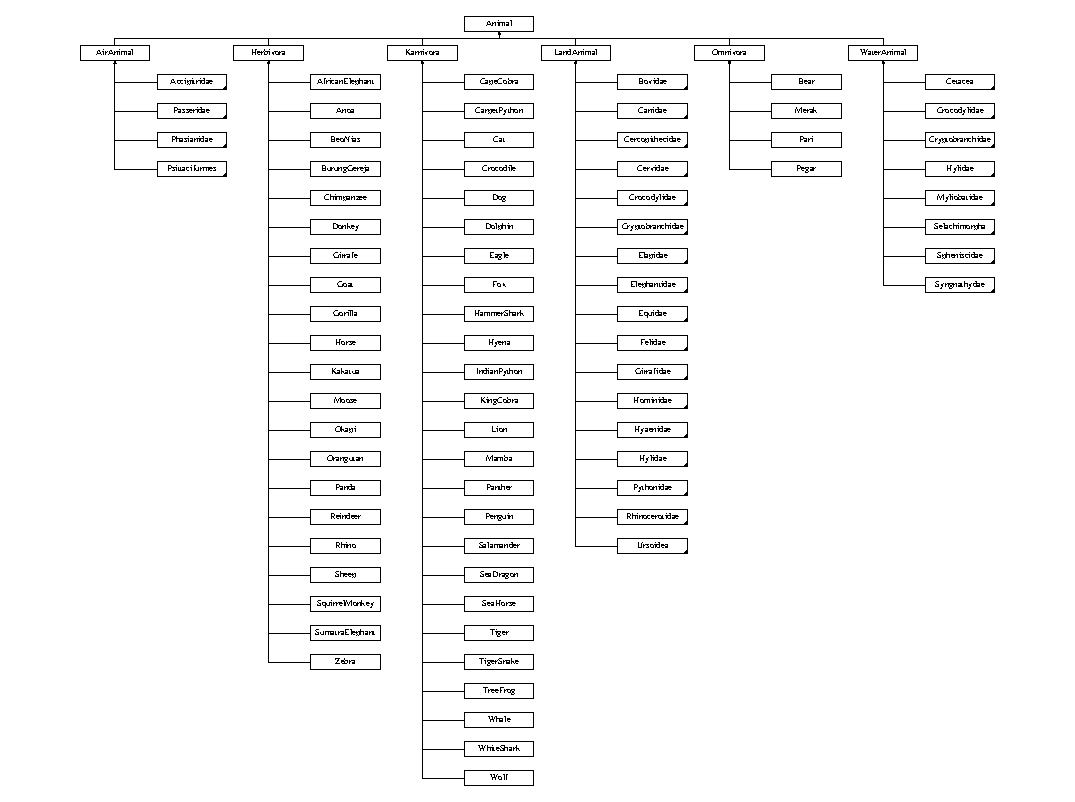
\includegraphics[height=10.327868cm]{class_animal}
\end{center}
\end{figure}
\subsection*{Public Member Functions}
\begin{DoxyCompactItemize}
\item 
\hyperlink{class_animal_a1e726a49ec952443190ac62dad22353c}{Animal} ()\hypertarget{class_animal_a1e726a49ec952443190ac62dad22353c}{}\label{class_animal_a1e726a49ec952443190ac62dad22353c}

\begin{DoxyCompactList}\small\item\em Constructor. \end{DoxyCompactList}\item 
virtual \hyperlink{class_animal_a476af25adde5f0dfa688129c8f86fa5c}{$\sim$\+Animal} ()\hypertarget{class_animal_a476af25adde5f0dfa688129c8f86fa5c}{}\label{class_animal_a476af25adde5f0dfa688129c8f86fa5c}

\begin{DoxyCompactList}\small\item\em Destructor. \end{DoxyCompactList}\item 
virtual void \hyperlink{class_animal_aa8f3017b9c7e36e0a43a0846eff27e9b}{Get\+Experience} ()\hypertarget{class_animal_aa8f3017b9c7e36e0a43a0846eff27e9b}{}\label{class_animal_aa8f3017b9c7e36e0a43a0846eff27e9b}

\begin{DoxyCompactList}\small\item\em Komunikasi dengan hewan. \end{DoxyCompactList}\item 
virtual int \hyperlink{class_animal_a9fdf4c4a5edd1265d9e0652127face39}{Get\+Food\+Num} ()=0
\begin{DoxyCompactList}\small\item\em Jumlah makanan. \end{DoxyCompactList}\item 
char \hyperlink{class_animal_a2573e109ec7241db7ed3eeb6363ee971}{Get\+Render} ()
\begin{DoxyCompactList}\small\item\em Print karakter. \end{DoxyCompactList}\item 
void \hyperlink{class_animal_a789dd4cdf9e115c253df5adf05656241}{Set\+Enemy} (char cc)
\begin{DoxyCompactList}\small\item\em Set karakter hewan. \end{DoxyCompactList}\item 
char $\ast$ \hyperlink{class_animal_a45be2a7ee0c91ad17626099acbd0a85d}{Get\+Enemy} ()
\begin{DoxyCompactList}\small\item\em Ambil list musuh. \end{DoxyCompactList}\item 
int $\ast$ \hyperlink{class_animal_aac38d92abcd76ecffa89eccffe76cdb6}{Get\+Type} ()
\begin{DoxyCompactList}\small\item\em Ambil tipe habitat hewan. \end{DoxyCompactList}\item 
int \hyperlink{class_animal_a9e9d7dece1f0f24eed4d51ef91b719ae}{Get\+Top\+Enemy} ()
\begin{DoxyCompactList}\small\item\em Ambil jumlah musuh. \end{DoxyCompactList}\item 
string \hyperlink{class_animal_a1a1ad83743b03fbe705721fa9dc23368}{Get\+Famili} ()
\begin{DoxyCompactList}\small\item\em Ambil Famili hewan. \end{DoxyCompactList}\item 
string \hyperlink{class_animal_ab96e4572871fa54d98cf639c6331ea90}{Get\+Species} ()
\begin{DoxyCompactList}\small\item\em Ambil species hewan. \end{DoxyCompactList}\item 
string \hyperlink{class_animal_a0f991dc05752ee65315e29ca3a1b5b11}{Get\+Isi\+Experience} ()
\begin{DoxyCompactList}\small\item\em Ambil experience hewan. \end{DoxyCompactList}\end{DoxyCompactItemize}
\subsection*{Protected Attributes}
\begin{DoxyCompactItemize}
\item 
int $\ast$ \hyperlink{class_animal_a0f113636c4f0a8ad73b1eba947a2e8e2}{type}
\item 
string \hyperlink{class_animal_aab17c94dd15ad3224c3c05ac74367be9}{famili}
\item 
string \hyperlink{class_animal_a70a223fc101b56962088b16a8b18534b}{species}
\item 
string \hyperlink{class_animal_a015f8fc08cd5e454b61d597805fa6e54}{experience}
\item 
short \hyperlink{class_animal_a703d6acefaa69242f9665c81f3e91c21}{jenis\+\_\+makanan}
\item 
int \hyperlink{class_animal_ad122855148e51ecfe706d099bb0eb6ac}{berat}
\item 
char \hyperlink{class_animal_a6a0e0157cbf3f766011629a9a8954326}{animal\+\_\+char}
\item 
char $\ast$ \hyperlink{class_animal_ae219f1b898b5e6afed1ecad4375b8124}{enemy\+\_\+char}
\item 
int \hyperlink{class_animal_a6620fb4081b171927278a00638d8d2d9}{top\+\_\+enemy}
\end{DoxyCompactItemize}


\subsection{Member Function Documentation}
\index{Animal@{Animal}!Get\+Enemy@{Get\+Enemy}}
\index{Get\+Enemy@{Get\+Enemy}!Animal@{Animal}}
\subsubsection[{\texorpdfstring{Get\+Enemy()}{GetEnemy()}}]{\setlength{\rightskip}{0pt plus 5cm}char $\ast$ Animal\+::\+Get\+Enemy (
\begin{DoxyParamCaption}
{}
\end{DoxyParamCaption}
)}\hypertarget{class_animal_a45be2a7ee0c91ad17626099acbd0a85d}{}\label{class_animal_a45be2a7ee0c91ad17626099acbd0a85d}


Ambil list musuh. 

\begin{DoxyReturn}{Returns}
List Musuh 
\end{DoxyReturn}
\index{Animal@{Animal}!Get\+Famili@{Get\+Famili}}
\index{Get\+Famili@{Get\+Famili}!Animal@{Animal}}
\subsubsection[{\texorpdfstring{Get\+Famili()}{GetFamili()}}]{\setlength{\rightskip}{0pt plus 5cm}string Animal\+::\+Get\+Famili (
\begin{DoxyParamCaption}
{}
\end{DoxyParamCaption}
)}\hypertarget{class_animal_a1a1ad83743b03fbe705721fa9dc23368}{}\label{class_animal_a1a1ad83743b03fbe705721fa9dc23368}


Ambil Famili hewan. 

Ambil famili hewan.

\begin{DoxyReturn}{Returns}
string famili 
\end{DoxyReturn}
\index{Animal@{Animal}!Get\+Food\+Num@{Get\+Food\+Num}}
\index{Get\+Food\+Num@{Get\+Food\+Num}!Animal@{Animal}}
\subsubsection[{\texorpdfstring{Get\+Food\+Num()=0}{GetFoodNum()=0}}]{\setlength{\rightskip}{0pt plus 5cm}virtual int Animal\+::\+Get\+Food\+Num (
\begin{DoxyParamCaption}
{}
\end{DoxyParamCaption}
)\hspace{0.3cm}{\ttfamily [pure virtual]}}\hypertarget{class_animal_a9fdf4c4a5edd1265d9e0652127face39}{}\label{class_animal_a9fdf4c4a5edd1265d9e0652127face39}


Jumlah makanan. 

\begin{DoxyReturn}{Returns}
Jumlah makan 
\end{DoxyReturn}


Implemented in \hyperlink{class_herbivora_ad23ef13a082b2efce54f9c9e3a33ab18}{Herbivora}, \hyperlink{class_karnivora_a1b61557ede78893f8a3f7c4fbd061c16}{Karnivora}, and \hyperlink{class_omnivora_af78063c104f28eb8662387c45abdc717}{Omnivora}.

\index{Animal@{Animal}!Get\+Isi\+Experience@{Get\+Isi\+Experience}}
\index{Get\+Isi\+Experience@{Get\+Isi\+Experience}!Animal@{Animal}}
\subsubsection[{\texorpdfstring{Get\+Isi\+Experience()}{GetIsiExperience()}}]{\setlength{\rightskip}{0pt plus 5cm}string Animal\+::\+Get\+Isi\+Experience (
\begin{DoxyParamCaption}
{}
\end{DoxyParamCaption}
)}\hypertarget{class_animal_a0f991dc05752ee65315e29ca3a1b5b11}{}\label{class_animal_a0f991dc05752ee65315e29ca3a1b5b11}


Ambil experience hewan. 

\begin{DoxyReturn}{Returns}
string experience 
\end{DoxyReturn}
\index{Animal@{Animal}!Get\+Render@{Get\+Render}}
\index{Get\+Render@{Get\+Render}!Animal@{Animal}}
\subsubsection[{\texorpdfstring{Get\+Render()}{GetRender()}}]{\setlength{\rightskip}{0pt plus 5cm}char Animal\+::\+Get\+Render (
\begin{DoxyParamCaption}
{}
\end{DoxyParamCaption}
)}\hypertarget{class_animal_a2573e109ec7241db7ed3eeb6363ee971}{}\label{class_animal_a2573e109ec7241db7ed3eeb6363ee971}


Print karakter. 

\begin{DoxyReturn}{Returns}
char 
\end{DoxyReturn}
\index{Animal@{Animal}!Get\+Species@{Get\+Species}}
\index{Get\+Species@{Get\+Species}!Animal@{Animal}}
\subsubsection[{\texorpdfstring{Get\+Species()}{GetSpecies()}}]{\setlength{\rightskip}{0pt plus 5cm}string Animal\+::\+Get\+Species (
\begin{DoxyParamCaption}
{}
\end{DoxyParamCaption}
)}\hypertarget{class_animal_ab96e4572871fa54d98cf639c6331ea90}{}\label{class_animal_ab96e4572871fa54d98cf639c6331ea90}


Ambil species hewan. 

\begin{DoxyReturn}{Returns}
string species 
\end{DoxyReturn}
\index{Animal@{Animal}!Get\+Top\+Enemy@{Get\+Top\+Enemy}}
\index{Get\+Top\+Enemy@{Get\+Top\+Enemy}!Animal@{Animal}}
\subsubsection[{\texorpdfstring{Get\+Top\+Enemy()}{GetTopEnemy()}}]{\setlength{\rightskip}{0pt plus 5cm}int Animal\+::\+Get\+Top\+Enemy (
\begin{DoxyParamCaption}
{}
\end{DoxyParamCaption}
)}\hypertarget{class_animal_a9e9d7dece1f0f24eed4d51ef91b719ae}{}\label{class_animal_a9e9d7dece1f0f24eed4d51ef91b719ae}


Ambil jumlah musuh. 

dapat jumlah musuh

\begin{DoxyReturn}{Returns}
int musuh

jumlah musuh 
\end{DoxyReturn}
\index{Animal@{Animal}!Get\+Type@{Get\+Type}}
\index{Get\+Type@{Get\+Type}!Animal@{Animal}}
\subsubsection[{\texorpdfstring{Get\+Type()}{GetType()}}]{\setlength{\rightskip}{0pt plus 5cm}int $\ast$ Animal\+::\+Get\+Type (
\begin{DoxyParamCaption}
{}
\end{DoxyParamCaption}
)}\hypertarget{class_animal_aac38d92abcd76ecffa89eccffe76cdb6}{}\label{class_animal_aac38d92abcd76ecffa89eccffe76cdb6}


Ambil tipe habitat hewan. 

\begin{DoxyReturn}{Returns}
List habitat 
\end{DoxyReturn}
\index{Animal@{Animal}!Set\+Enemy@{Set\+Enemy}}
\index{Set\+Enemy@{Set\+Enemy}!Animal@{Animal}}
\subsubsection[{\texorpdfstring{Set\+Enemy(char cc)}{SetEnemy(char cc)}}]{\setlength{\rightskip}{0pt plus 5cm}void Animal\+::\+Set\+Enemy (
\begin{DoxyParamCaption}
\item[{char}]{cc}
\end{DoxyParamCaption}
)}\hypertarget{class_animal_a789dd4cdf9e115c253df5adf05656241}{}\label{class_animal_a789dd4cdf9e115c253df5adf05656241}


Set karakter hewan. 


\begin{DoxyParams}{Parameters}
{\em cc} & Karakter hewan tsb \\
\hline
\end{DoxyParams}


\subsection{Member Data Documentation}
\index{Animal@{Animal}!animal\+\_\+char@{animal\+\_\+char}}
\index{animal\+\_\+char@{animal\+\_\+char}!Animal@{Animal}}
\subsubsection[{\texorpdfstring{animal\+\_\+char}{animal_char}}]{\setlength{\rightskip}{0pt plus 5cm}char Animal\+::animal\+\_\+char\hspace{0.3cm}{\ttfamily [protected]}}\hypertarget{class_animal_a6a0e0157cbf3f766011629a9a8954326}{}\label{class_animal_a6a0e0157cbf3f766011629a9a8954326}
Char yang digunakan untuk render \index{Animal@{Animal}!berat@{berat}}
\index{berat@{berat}!Animal@{Animal}}
\subsubsection[{\texorpdfstring{berat}{berat}}]{\setlength{\rightskip}{0pt plus 5cm}int Animal\+::berat\hspace{0.3cm}{\ttfamily [protected]}}\hypertarget{class_animal_ad122855148e51ecfe706d099bb0eb6ac}{}\label{class_animal_ad122855148e51ecfe706d099bb0eb6ac}
Berat hewan \index{Animal@{Animal}!enemy\+\_\+char@{enemy\+\_\+char}}
\index{enemy\+\_\+char@{enemy\+\_\+char}!Animal@{Animal}}
\subsubsection[{\texorpdfstring{enemy\+\_\+char}{enemy_char}}]{\setlength{\rightskip}{0pt plus 5cm}char$\ast$ Animal\+::enemy\+\_\+char\hspace{0.3cm}{\ttfamily [protected]}}\hypertarget{class_animal_ae219f1b898b5e6afed1ecad4375b8124}{}\label{class_animal_ae219f1b898b5e6afed1ecad4375b8124}
Array of char yang berisi list musuhnya \index{Animal@{Animal}!experience@{experience}}
\index{experience@{experience}!Animal@{Animal}}
\subsubsection[{\texorpdfstring{experience}{experience}}]{\setlength{\rightskip}{0pt plus 5cm}string Animal\+::experience\hspace{0.3cm}{\ttfamily [protected]}}\hypertarget{class_animal_a015f8fc08cd5e454b61d597805fa6e54}{}\label{class_animal_a015f8fc08cd5e454b61d597805fa6e54}
Experience hewan \index{Animal@{Animal}!famili@{famili}}
\index{famili@{famili}!Animal@{Animal}}
\subsubsection[{\texorpdfstring{famili}{famili}}]{\setlength{\rightskip}{0pt plus 5cm}string Animal\+::famili\hspace{0.3cm}{\ttfamily [protected]}}\hypertarget{class_animal_aab17c94dd15ad3224c3c05ac74367be9}{}\label{class_animal_aab17c94dd15ad3224c3c05ac74367be9}
Family hewan \index{Animal@{Animal}!jenis\+\_\+makanan@{jenis\+\_\+makanan}}
\index{jenis\+\_\+makanan@{jenis\+\_\+makanan}!Animal@{Animal}}
\subsubsection[{\texorpdfstring{jenis\+\_\+makanan}{jenis_makanan}}]{\setlength{\rightskip}{0pt plus 5cm}short Animal\+::jenis\+\_\+makanan\hspace{0.3cm}{\ttfamily [protected]}}\hypertarget{class_animal_a703d6acefaa69242f9665c81f3e91c21}{}\label{class_animal_a703d6acefaa69242f9665c81f3e91c21}
Jenis Makanan hewan. 1 \+: herbifor, 2 \+: karnivor, 3 \+: omnifor \index{Animal@{Animal}!species@{species}}
\index{species@{species}!Animal@{Animal}}
\subsubsection[{\texorpdfstring{species}{species}}]{\setlength{\rightskip}{0pt plus 5cm}string Animal\+::species\hspace{0.3cm}{\ttfamily [protected]}}\hypertarget{class_animal_a70a223fc101b56962088b16a8b18534b}{}\label{class_animal_a70a223fc101b56962088b16a8b18534b}
Species hewan \index{Animal@{Animal}!top\+\_\+enemy@{top\+\_\+enemy}}
\index{top\+\_\+enemy@{top\+\_\+enemy}!Animal@{Animal}}
\subsubsection[{\texorpdfstring{top\+\_\+enemy}{top_enemy}}]{\setlength{\rightskip}{0pt plus 5cm}int Animal\+::top\+\_\+enemy\hspace{0.3cm}{\ttfamily [protected]}}\hypertarget{class_animal_a6620fb4081b171927278a00638d8d2d9}{}\label{class_animal_a6620fb4081b171927278a00638d8d2d9}
Pointer Enemy\+Char yang available \index{Animal@{Animal}!type@{type}}
\index{type@{type}!Animal@{Animal}}
\subsubsection[{\texorpdfstring{type}{type}}]{\setlength{\rightskip}{0pt plus 5cm}int$\ast$ Animal\+::type\hspace{0.3cm}{\ttfamily [protected]}}\hypertarget{class_animal_a0f113636c4f0a8ad73b1eba947a2e8e2}{}\label{class_animal_a0f113636c4f0a8ad73b1eba947a2e8e2}
Type habitat hewan. 0 \+: darat, 1 \+: udara, 2 \+: air 

The documentation for this class was generated from the following files\+:\begin{DoxyCompactItemize}
\item 
animal.\+h\item 
animal.\+cpp\end{DoxyCompactItemize}

\hypertarget{class_anoa}{}\section{Anoa Class Reference}
\label{class_anoa}\index{Anoa@{Anoa}}
\subsection*{Public Member Functions}
\begin{DoxyCompactItemize}
\item 
\hyperlink{class_anoa_adc03b4c166e61ef3c66c84bb9f74d037}{Anoa} ()\hypertarget{class_anoa_adc03b4c166e61ef3c66c84bb9f74d037}{}\label{class_anoa_adc03b4c166e61ef3c66c84bb9f74d037}

\begin{DoxyCompactList}\small\item\em Inisialisasi Hewan. \end{DoxyCompactList}\item 
\hyperlink{class_anoa_ab80d0e5f30d7b6a008e56f4fad144ecf}{$\sim$\+Anoa} ()\hypertarget{class_anoa_ab80d0e5f30d7b6a008e56f4fad144ecf}{}\label{class_anoa_ab80d0e5f30d7b6a008e56f4fad144ecf}

\begin{DoxyCompactList}\small\item\em Destructor. \end{DoxyCompactList}\item 
string \hyperlink{class_anoa_a5873ad7fbbaabe159fe78d18abca5cf9}{Get\+Experience} ()\hypertarget{class_anoa_a5873ad7fbbaabe159fe78d18abca5cf9}{}\label{class_anoa_a5873ad7fbbaabe159fe78d18abca5cf9}

\begin{DoxyCompactList}\small\item\em Komunikasi dengan hewan. \end{DoxyCompactList}\item 
int \hyperlink{class_anoa_a1bd6ef587f919996a80664ce7fe378f4}{Get\+Food\+Num} ()
\begin{DoxyCompactList}\small\item\em Jumlah makanan. \end{DoxyCompactList}\item 
char \hyperlink{class_anoa_aa18da9e26b96be2ab14510cab0753653}{Get\+Render} ()
\begin{DoxyCompactList}\small\item\em Print karakter. \end{DoxyCompactList}\item 
void \hyperlink{class_anoa_a3e2a743b367371207a4f511542016c9f}{Set\+Enemy} (char cc)
\begin{DoxyCompactList}\small\item\em Set karakter hewan. \end{DoxyCompactList}\item 
char $\ast$ \hyperlink{class_anoa_aebfc13ce0edf718e7ad691ce227444dc}{Get\+Enemy} ()
\begin{DoxyCompactList}\small\item\em Ambil list musuh. \end{DoxyCompactList}\end{DoxyCompactItemize}
\subsection*{Protected Attributes}
\begin{DoxyCompactItemize}
\item 
int $\ast$ \hyperlink{class_anoa_a074ddc510aa6b04d78100f1d9d562f2e}{Type}
\item 
string \hyperlink{class_anoa_a70b854fa12421457338081ff66e23b3c}{Famili}
\item 
string \hyperlink{class_anoa_a6dffd5df83dbf71071233b6c32aac878}{Species}
\item 
string \hyperlink{class_anoa_a6791e3fbe425ec1b478dcf2544c039aa}{Experience}
\item 
short \hyperlink{class_anoa_af710bb7dedfd5ea717db3c940981d3e9}{Jenis\+Makanan}
\item 
int \hyperlink{class_anoa_ace1d7758a5e8371a22b23fecbf9152e7}{Berat}
\item 
char \hyperlink{class_anoa_a4bfb9cb19e5c6c784d8e60b060f7fa7f}{Ani\+Char}
\item 
char $\ast$ \hyperlink{class_anoa_abc7657c0df0c0a08b69c9fd9213442f2}{Enemy\+Char}
\item 
int \hyperlink{class_anoa_ae36a4e73eaeed7952baf5804ea68cdc2}{Top\+Enemy}
\end{DoxyCompactItemize}


\subsection{Member Function Documentation}
\index{Anoa@{Anoa}!Get\+Enemy@{Get\+Enemy}}
\index{Get\+Enemy@{Get\+Enemy}!Anoa@{Anoa}}
\subsubsection[{\texorpdfstring{Get\+Enemy()}{GetEnemy()}}]{\setlength{\rightskip}{0pt plus 5cm}char $\ast$ Anoa\+::\+Get\+Enemy (
\begin{DoxyParamCaption}
{}
\end{DoxyParamCaption}
)}\hypertarget{class_anoa_aebfc13ce0edf718e7ad691ce227444dc}{}\label{class_anoa_aebfc13ce0edf718e7ad691ce227444dc}


Ambil list musuh. 

\begin{DoxyReturn}{Returns}
List Musuh 
\end{DoxyReturn}
\index{Anoa@{Anoa}!Get\+Food\+Num@{Get\+Food\+Num}}
\index{Get\+Food\+Num@{Get\+Food\+Num}!Anoa@{Anoa}}
\subsubsection[{\texorpdfstring{Get\+Food\+Num()}{GetFoodNum()}}]{\setlength{\rightskip}{0pt plus 5cm}int Anoa\+::\+Get\+Food\+Num (
\begin{DoxyParamCaption}
{}
\end{DoxyParamCaption}
)}\hypertarget{class_anoa_a1bd6ef587f919996a80664ce7fe378f4}{}\label{class_anoa_a1bd6ef587f919996a80664ce7fe378f4}


Jumlah makanan. 

\begin{DoxyReturn}{Returns}
Jumlah makan

Jumlah makanan 
\end{DoxyReturn}
\index{Anoa@{Anoa}!Get\+Render@{Get\+Render}}
\index{Get\+Render@{Get\+Render}!Anoa@{Anoa}}
\subsubsection[{\texorpdfstring{Get\+Render()}{GetRender()}}]{\setlength{\rightskip}{0pt plus 5cm}char Anoa\+::\+Get\+Render (
\begin{DoxyParamCaption}
{}
\end{DoxyParamCaption}
)}\hypertarget{class_anoa_aa18da9e26b96be2ab14510cab0753653}{}\label{class_anoa_aa18da9e26b96be2ab14510cab0753653}


Print karakter. 

\begin{DoxyReturn}{Returns}
char 
\end{DoxyReturn}
\index{Anoa@{Anoa}!Set\+Enemy@{Set\+Enemy}}
\index{Set\+Enemy@{Set\+Enemy}!Anoa@{Anoa}}
\subsubsection[{\texorpdfstring{Set\+Enemy(char cc)}{SetEnemy(char cc)}}]{\setlength{\rightskip}{0pt plus 5cm}void Anoa\+::\+Set\+Enemy (
\begin{DoxyParamCaption}
\item[{char}]{cc}
\end{DoxyParamCaption}
)}\hypertarget{class_anoa_a3e2a743b367371207a4f511542016c9f}{}\label{class_anoa_a3e2a743b367371207a4f511542016c9f}


Set karakter hewan. 


\begin{DoxyParams}{Parameters}
{\em cc} & Karakter hewan tsb \\
\hline
\end{DoxyParams}


\subsection{Member Data Documentation}
\index{Anoa@{Anoa}!Ani\+Char@{Ani\+Char}}
\index{Ani\+Char@{Ani\+Char}!Anoa@{Anoa}}
\subsubsection[{\texorpdfstring{Ani\+Char}{AniChar}}]{\setlength{\rightskip}{0pt plus 5cm}char Anoa\+::\+Ani\+Char\hspace{0.3cm}{\ttfamily [protected]}}\hypertarget{class_anoa_a4bfb9cb19e5c6c784d8e60b060f7fa7f}{}\label{class_anoa_a4bfb9cb19e5c6c784d8e60b060f7fa7f}
Char yang digunakan untuk render \index{Anoa@{Anoa}!Berat@{Berat}}
\index{Berat@{Berat}!Anoa@{Anoa}}
\subsubsection[{\texorpdfstring{Berat}{Berat}}]{\setlength{\rightskip}{0pt plus 5cm}int Anoa\+::\+Berat\hspace{0.3cm}{\ttfamily [protected]}}\hypertarget{class_anoa_ace1d7758a5e8371a22b23fecbf9152e7}{}\label{class_anoa_ace1d7758a5e8371a22b23fecbf9152e7}
Berat hewan \index{Anoa@{Anoa}!Enemy\+Char@{Enemy\+Char}}
\index{Enemy\+Char@{Enemy\+Char}!Anoa@{Anoa}}
\subsubsection[{\texorpdfstring{Enemy\+Char}{EnemyChar}}]{\setlength{\rightskip}{0pt plus 5cm}char$\ast$ Anoa\+::\+Enemy\+Char\hspace{0.3cm}{\ttfamily [protected]}}\hypertarget{class_anoa_abc7657c0df0c0a08b69c9fd9213442f2}{}\label{class_anoa_abc7657c0df0c0a08b69c9fd9213442f2}
Array of char yang berisi list musuhnya \index{Anoa@{Anoa}!Experience@{Experience}}
\index{Experience@{Experience}!Anoa@{Anoa}}
\subsubsection[{\texorpdfstring{Experience}{Experience}}]{\setlength{\rightskip}{0pt plus 5cm}string Anoa\+::\+Experience\hspace{0.3cm}{\ttfamily [protected]}}\hypertarget{class_anoa_a6791e3fbe425ec1b478dcf2544c039aa}{}\label{class_anoa_a6791e3fbe425ec1b478dcf2544c039aa}
Experience hewan \index{Anoa@{Anoa}!Famili@{Famili}}
\index{Famili@{Famili}!Anoa@{Anoa}}
\subsubsection[{\texorpdfstring{Famili}{Famili}}]{\setlength{\rightskip}{0pt plus 5cm}string Anoa\+::\+Famili\hspace{0.3cm}{\ttfamily [protected]}}\hypertarget{class_anoa_a70b854fa12421457338081ff66e23b3c}{}\label{class_anoa_a70b854fa12421457338081ff66e23b3c}
Family hewan \index{Anoa@{Anoa}!Jenis\+Makanan@{Jenis\+Makanan}}
\index{Jenis\+Makanan@{Jenis\+Makanan}!Anoa@{Anoa}}
\subsubsection[{\texorpdfstring{Jenis\+Makanan}{JenisMakanan}}]{\setlength{\rightskip}{0pt plus 5cm}short Anoa\+::\+Jenis\+Makanan\hspace{0.3cm}{\ttfamily [protected]}}\hypertarget{class_anoa_af710bb7dedfd5ea717db3c940981d3e9}{}\label{class_anoa_af710bb7dedfd5ea717db3c940981d3e9}
Jenis Makanan hewan. 1 \+: herbifor, 2 \+: karnivor, 3 \+: omnifor \index{Anoa@{Anoa}!Species@{Species}}
\index{Species@{Species}!Anoa@{Anoa}}
\subsubsection[{\texorpdfstring{Species}{Species}}]{\setlength{\rightskip}{0pt plus 5cm}string Anoa\+::\+Species\hspace{0.3cm}{\ttfamily [protected]}}\hypertarget{class_anoa_a6dffd5df83dbf71071233b6c32aac878}{}\label{class_anoa_a6dffd5df83dbf71071233b6c32aac878}
Species hewan \index{Anoa@{Anoa}!Top\+Enemy@{Top\+Enemy}}
\index{Top\+Enemy@{Top\+Enemy}!Anoa@{Anoa}}
\subsubsection[{\texorpdfstring{Top\+Enemy}{TopEnemy}}]{\setlength{\rightskip}{0pt plus 5cm}int Anoa\+::\+Top\+Enemy\hspace{0.3cm}{\ttfamily [protected]}}\hypertarget{class_anoa_ae36a4e73eaeed7952baf5804ea68cdc2}{}\label{class_anoa_ae36a4e73eaeed7952baf5804ea68cdc2}
Pointer Enemy\+Char yang available \index{Anoa@{Anoa}!Type@{Type}}
\index{Type@{Type}!Anoa@{Anoa}}
\subsubsection[{\texorpdfstring{Type}{Type}}]{\setlength{\rightskip}{0pt plus 5cm}int$\ast$ Anoa\+::\+Type\hspace{0.3cm}{\ttfamily [protected]}}\hypertarget{class_anoa_a074ddc510aa6b04d78100f1d9d562f2e}{}\label{class_anoa_a074ddc510aa6b04d78100f1d9d562f2e}
Type habitat hewan. 0 \+: darat, 1 \+: udara, 2 \+: air 

The documentation for this class was generated from the following files\+:\begin{DoxyCompactItemize}
\item 
anoa.\+h\item 
anoa.\+cpp\end{DoxyCompactItemize}

\hypertarget{class_bear}{}\section{Bear Class Reference}
\label{class_bear}\index{Bear@{Bear}}
Inheritance diagram for Bear\+:\begin{figure}[H]
\begin{center}
\leavevmode
\includegraphics[height=4.000000cm]{class_bear}
\end{center}
\end{figure}
\subsection*{Public Member Functions}
\begin{DoxyCompactItemize}
\item 
\hyperlink{class_bear_a639d2d41ec84454055f7b44f23c39639}{Bear} ()\hypertarget{class_bear_a639d2d41ec84454055f7b44f23c39639}{}\label{class_bear_a639d2d41ec84454055f7b44f23c39639}

\begin{DoxyCompactList}\small\item\em Inisialisasi Hewan. \end{DoxyCompactList}\end{DoxyCompactItemize}
\subsection*{Additional Inherited Members}


The documentation for this class was generated from the following files\+:\begin{DoxyCompactItemize}
\item 
land\+\_\+animal.\+h\item 
land\+\_\+animal.\+cpp\end{DoxyCompactItemize}

\hypertarget{class_beo_nias}{}\section{Beo\+Nias Class Reference}
\label{class_beo_nias}\index{Beo\+Nias@{Beo\+Nias}}
Inheritance diagram for Beo\+Nias\+:\begin{figure}[H]
\begin{center}
\leavevmode
\includegraphics[height=4.000000cm]{class_beo_nias}
\end{center}
\end{figure}
\subsection*{Public Member Functions}
\begin{DoxyCompactItemize}
\item 
\hyperlink{class_beo_nias_a194bc47e9a3b814159d7ac4a43293b1c}{Beo\+Nias} ()\hypertarget{class_beo_nias_a194bc47e9a3b814159d7ac4a43293b1c}{}\label{class_beo_nias_a194bc47e9a3b814159d7ac4a43293b1c}

\begin{DoxyCompactList}\small\item\em Inisialisasi Hewan. \end{DoxyCompactList}\end{DoxyCompactItemize}
\subsection*{Additional Inherited Members}


The documentation for this class was generated from the following files\+:\begin{DoxyCompactItemize}
\item 
air\+\_\+animal.\+h\item 
air\+\_\+animal.\+cpp\end{DoxyCompactItemize}

\hypertarget{class_bovidae}{}\section{Bovidae Class Reference}
\label{class_bovidae}\index{Bovidae@{Bovidae}}
Inheritance diagram for Bovidae\+:\begin{figure}[H]
\begin{center}
\leavevmode
\includegraphics[height=4.000000cm]{class_bovidae}
\end{center}
\end{figure}
\subsection*{Public Member Functions}
\begin{DoxyCompactItemize}
\item 
\hyperlink{class_bovidae_aaf97900f7eaef28ee3ff7304d68b3f7c}{Bovidae} ()\hypertarget{class_bovidae_aaf97900f7eaef28ee3ff7304d68b3f7c}{}\label{class_bovidae_aaf97900f7eaef28ee3ff7304d68b3f7c}

\begin{DoxyCompactList}\small\item\em Inisialisasi Famili. \end{DoxyCompactList}\end{DoxyCompactItemize}
\subsection*{Additional Inherited Members}


The documentation for this class was generated from the following files\+:\begin{DoxyCompactItemize}
\item 
land\+\_\+animal.\+h\item 
land\+\_\+animal.\+cpp\end{DoxyCompactItemize}

\hypertarget{class_burung_gereja}{}\section{Burung\+Gereja Class Reference}
\label{class_burung_gereja}\index{Burung\+Gereja@{Burung\+Gereja}}
Inheritance diagram for Burung\+Gereja\+:\begin{figure}[H]
\begin{center}
\leavevmode
\includegraphics[height=4.000000cm]{class_burung_gereja}
\end{center}
\end{figure}
\subsection*{Public Member Functions}
\begin{DoxyCompactItemize}
\item 
\hyperlink{class_burung_gereja_a1af7e3d1cd28dc627a6c61c21baf99b2}{Burung\+Gereja} ()\hypertarget{class_burung_gereja_a1af7e3d1cd28dc627a6c61c21baf99b2}{}\label{class_burung_gereja_a1af7e3d1cd28dc627a6c61c21baf99b2}

\begin{DoxyCompactList}\small\item\em Inisialisasi Hewan. \end{DoxyCompactList}\end{DoxyCompactItemize}
\subsection*{Additional Inherited Members}


The documentation for this class was generated from the following files\+:\begin{DoxyCompactItemize}
\item 
air\+\_\+animal.\+h\item 
air\+\_\+animal.\+cpp\end{DoxyCompactItemize}

\hypertarget{class_cage}{}\section{Cage Class Reference}
\label{class_cage}\index{Cage@{Cage}}
Inheritance diagram for Cage\+:\begin{figure}[H]
\begin{center}
\leavevmode
\includegraphics[height=2.000000cm]{class_cage}
\end{center}
\end{figure}
\subsection*{Public Member Functions}
\begin{DoxyCompactItemize}
\item 
\hyperlink{class_cage_a60e37f6ee39538735bddde13e91a9758}{Cage} (int \hyperlink{class_cage_a84ab0098eebdb6ce6d00a64533eb963c}{Hab\+Type}, int \hyperlink{class_cage_a4e04166edf60c708910a7b1c6d81bf3a}{Jumlah\+Animal}, int Max\+Luas\+Cage)
\begin{DoxyCompactList}\small\item\em Constructor. \end{DoxyCompactList}\item 
void \hyperlink{class_cage_ac7b058e3bcad6642edcc1078a393ceb8}{Add\+Animal} (\hyperlink{class_animal}{Animal} $\ast$Ani, int x, int y)
\begin{DoxyCompactList}\small\item\em Menambah \hyperlink{class_animal}{Animal} ke point tertentu. \end{DoxyCompactList}\item 
void \hyperlink{class_cage_a449f19d08289f70a140955a99769ae4a}{Move} ()\hypertarget{class_cage_a449f19d08289f70a140955a99769ae4a}{}\label{class_cage_a449f19d08289f70a140955a99769ae4a}

\begin{DoxyCompactList}\small\item\em Gerak. \end{DoxyCompactList}\item 
virtual \hyperlink{class_cage_a657259499dfc23c63fc65aeaf8abbb17}{$\sim$\+Cage} ()\hypertarget{class_cage_a657259499dfc23c63fc65aeaf8abbb17}{}\label{class_cage_a657259499dfc23c63fc65aeaf8abbb17}

\begin{DoxyCompactList}\small\item\em Destructor. \end{DoxyCompactList}\item 
void \hyperlink{class_cage_a6cf474c9514e4ed3b344ae11548a15ad}{Set\+Cage\+Num} (int x)
\begin{DoxyCompactList}\small\item\em Jumlah\+Cage. \end{DoxyCompactList}\item 
int {\bfseries Get\+Cage\+Num} ()\hypertarget{class_cage_a46e5715ddcb28e5a2d7f79884f28a90a}{}\label{class_cage_a46e5715ddcb28e5a2d7f79884f28a90a}

\item 
void \hyperlink{class_cage_aec2f91bbd16b0997b787ac0cc8afa5b5}{Add\+Habitat} (\hyperlink{class_habitat}{Habitat} $\ast$H)
\begin{DoxyCompactList}\small\item\em Menambahkan \hyperlink{class_habitat}{Habitat}. \end{DoxyCompactList}\item 
void \hyperlink{class_cage_ac0bc91af45c6eb9a8174c4387310348d}{Show\+Hewan} ()\hypertarget{class_cage_ac0bc91af45c6eb9a8174c4387310348d}{}\label{class_cage_ac0bc91af45c6eb9a8174c4387310348d}

\begin{DoxyCompactList}\small\item\em Menunjukkan Hewan. \end{DoxyCompactList}\item 
int \hyperlink{class_cage_a4aaadecb8628c82e3611cc3bf99df9b3}{Jumlah\+Makan\+Kandang} ()
\begin{DoxyCompactList}\small\item\em Total Makanan. \end{DoxyCompactList}\item 
void \hyperlink{class_cage_aabfee407ec4cff7ef83e122611244a07}{render} (char $\ast$$\ast$cc)
\begin{DoxyCompactList}\small\item\em Menambahkan \hyperlink{class_habitat}{Habitat}. \end{DoxyCompactList}\end{DoxyCompactItemize}
\subsection*{Protected Member Functions}
\begin{DoxyCompactItemize}
\item 
bool {\bfseries Is\+In\+Cage} (int x, int y)\hypertarget{class_cage_a72145e1ca4fc9716d09ba1bcf3ae6bf3}{}\label{class_cage_a72145e1ca4fc9716d09ba1bcf3ae6bf3}

\item 
bool {\bfseries Ada\+Animal} (int x, int y)\hypertarget{class_cage_a13297d663f6a114deeb56306756e8aa5}{}\label{class_cage_a13297d663f6a114deeb56306756e8aa5}

\item 
bool \hyperlink{class_cage_a53c42a46fc76605447aa08b7c51855c8}{Bisa\+Add\+Animal} (\hyperlink{class_animal}{Animal} $\ast$Ani, int x, int y)
\begin{DoxyCompactList}\small\item\em Menambah \hyperlink{class_animal}{Animal}. \end{DoxyCompactList}\end{DoxyCompactItemize}
\subsection*{Protected Attributes}
\begin{DoxyCompactItemize}
\item 
\hyperlink{class_animal}{Animal} $\ast$$\ast$ \hyperlink{class_cage_a6fa1c17b824da167225c5fe8bdba502f}{Ani\+Data}
\item 
\hyperlink{class_point}{Point} $\ast$ \hyperlink{class_cage_acf5ff40bfeaf9b5b34b2d8e3d856f3e9}{Ani\+Loc}
\item 
int \hyperlink{class_cage_a4e04166edf60c708910a7b1c6d81bf3a}{Jumlah\+Animal}
\item 
int \hyperlink{class_cage_a84ab0098eebdb6ce6d00a64533eb963c}{Hab\+Type}
\item 
int \hyperlink{class_cage_ab909423b207293975f4f486849e46db7}{Pointer\+Animal}
\item 
\hyperlink{class_point}{Point} $\ast$ \hyperlink{class_cage_a89c2490b6f2a07413b68922ba20facb9}{P}
\item 
int \hyperlink{class_cage_a5a1aeb70e196f3d5c7539b8277cd89c6}{Luas\+Cage}
\item 
int \hyperlink{class_cage_abfa1de5ec469c33b6495d2e5343b2ac1}{Pointer\+Point}
\item 
int \hyperlink{class_cage_ac5a1653970d687b3c6070580c203a88e}{Cage\+Num}
\end{DoxyCompactItemize}


\subsection{Constructor \& Destructor Documentation}
\index{Cage@{Cage}!Cage@{Cage}}
\index{Cage@{Cage}!Cage@{Cage}}
\subsubsection[{\texorpdfstring{Cage(int Hab\+Type, int Jumlah\+Animal, int Max\+Luas\+Cage)}{Cage(int HabType, int JumlahAnimal, int MaxLuasCage)}}]{\setlength{\rightskip}{0pt plus 5cm}Cage\+::\+Cage (
\begin{DoxyParamCaption}
\item[{int}]{habitat\+\_\+type, }
\item[{int}]{jumlah\+\_\+animal, }
\item[{int}]{max\+\_\+luas\+\_\+cage}
\end{DoxyParamCaption}
)}\hypertarget{class_cage_a60e37f6ee39538735bddde13e91a9758}{}\label{class_cage_a60e37f6ee39538735bddde13e91a9758}


Constructor. 


\begin{DoxyParams}{Parameters}
{\em Hab\+Type} & tipe habitat. \\
\hline
{\em Jumlah\+Animal.} & \\
\hline
{\em Max\+Luas\+Cage} & \\
\hline
{\em habitat\+\_\+type} & tipe habitat. \\
\hline
{\em jumlah\+\_\+animal.} & \\
\hline
{\em max\+\_\+luas\+\_\+cage} & \\
\hline
\end{DoxyParams}


\subsection{Member Function Documentation}
\index{Cage@{Cage}!Add\+Animal@{Add\+Animal}}
\index{Add\+Animal@{Add\+Animal}!Cage@{Cage}}
\subsubsection[{\texorpdfstring{Add\+Animal(\+Animal $\ast$\+Ani, int x, int y)}{AddAnimal(Animal *Ani, int x, int y)}}]{\setlength{\rightskip}{0pt plus 5cm}void Cage\+::\+Add\+Animal (
\begin{DoxyParamCaption}
\item[{{\bf Animal} $\ast$}]{Ani, }
\item[{int}]{x, }
\item[{int}]{y}
\end{DoxyParamCaption}
)}\hypertarget{class_cage_ac7b058e3bcad6642edcc1078a393ceb8}{}\label{class_cage_ac7b058e3bcad6642edcc1078a393ceb8}


Menambah \hyperlink{class_animal}{Animal} ke point tertentu. 


\begin{DoxyParams}{Parameters}
{\em Ani} & Hewan \\
\hline
{\em X} & posisi X \\
\hline
{\em Y} & posisi Y \\
\hline
\end{DoxyParams}
\index{Cage@{Cage}!Add\+Habitat@{Add\+Habitat}}
\index{Add\+Habitat@{Add\+Habitat}!Cage@{Cage}}
\subsubsection[{\texorpdfstring{Add\+Habitat(\+Habitat $\ast$\+H)}{AddHabitat(Habitat *H)}}]{\setlength{\rightskip}{0pt plus 5cm}void Cage\+::\+Add\+Habitat (
\begin{DoxyParamCaption}
\item[{{\bf Habitat} $\ast$}]{H}
\end{DoxyParamCaption}
)}\hypertarget{class_cage_aec2f91bbd16b0997b787ac0cc8afa5b5}{}\label{class_cage_aec2f91bbd16b0997b787ac0cc8afa5b5}


Menambahkan \hyperlink{class_habitat}{Habitat}. 


\begin{DoxyParams}{Parameters}
{\em H} & \hyperlink{class_habitat}{Habitat} \\
\hline
\end{DoxyParams}
\index{Cage@{Cage}!Bisa\+Add\+Animal@{Bisa\+Add\+Animal}}
\index{Bisa\+Add\+Animal@{Bisa\+Add\+Animal}!Cage@{Cage}}
\subsubsection[{\texorpdfstring{Bisa\+Add\+Animal(\+Animal $\ast$\+Ani, int x, int y)}{BisaAddAnimal(Animal *Ani, int x, int y)}}]{\setlength{\rightskip}{0pt plus 5cm}bool Cage\+::\+Bisa\+Add\+Animal (
\begin{DoxyParamCaption}
\item[{{\bf Animal} $\ast$}]{Ani, }
\item[{int}]{x, }
\item[{int}]{y}
\end{DoxyParamCaption}
)\hspace{0.3cm}{\ttfamily [protected]}}\hypertarget{class_cage_a53c42a46fc76605447aa08b7c51855c8}{}\label{class_cage_a53c42a46fc76605447aa08b7c51855c8}


Menambah \hyperlink{class_animal}{Animal}. 


\begin{DoxyParams}{Parameters}
{\em Ani} & Hewan \\
\hline
{\em X} & posisi X \\
\hline
{\em Y} & posisi Y \\
\hline
\end{DoxyParams}
\index{Cage@{Cage}!Jumlah\+Makan\+Kandang@{Jumlah\+Makan\+Kandang}}
\index{Jumlah\+Makan\+Kandang@{Jumlah\+Makan\+Kandang}!Cage@{Cage}}
\subsubsection[{\texorpdfstring{Jumlah\+Makan\+Kandang()}{JumlahMakanKandang()}}]{\setlength{\rightskip}{0pt plus 5cm}int Cage\+::\+Jumlah\+Makan\+Kandang (
\begin{DoxyParamCaption}
{}
\end{DoxyParamCaption}
)}\hypertarget{class_cage_a4aaadecb8628c82e3611cc3bf99df9b3}{}\label{class_cage_a4aaadecb8628c82e3611cc3bf99df9b3}


Total Makanan. 

\begin{DoxyReturn}{Returns}
Jumlah makan tiap kandang

Jumlah Makan tiap Kandang 
\end{DoxyReturn}
\index{Cage@{Cage}!render@{render}}
\index{render@{render}!Cage@{Cage}}
\subsubsection[{\texorpdfstring{render(char $\ast$$\ast$cc)}{render(char **cc)}}]{\setlength{\rightskip}{0pt plus 5cm}void Cage\+::render (
\begin{DoxyParamCaption}
\item[{char $\ast$$\ast$}]{cc}
\end{DoxyParamCaption}
)}\hypertarget{class_cage_aabfee407ec4cff7ef83e122611244a07}{}\label{class_cage_aabfee407ec4cff7ef83e122611244a07}


Menambahkan \hyperlink{class_habitat}{Habitat}. 


\begin{DoxyParams}{Parameters}
{\em cc} & Nawn \\
\hline
\end{DoxyParams}
\index{Cage@{Cage}!Set\+Cage\+Num@{Set\+Cage\+Num}}
\index{Set\+Cage\+Num@{Set\+Cage\+Num}!Cage@{Cage}}
\subsubsection[{\texorpdfstring{Set\+Cage\+Num(int x)}{SetCageNum(int x)}}]{\setlength{\rightskip}{0pt plus 5cm}void Cage\+::\+Set\+Cage\+Num (
\begin{DoxyParamCaption}
\item[{int}]{x}
\end{DoxyParamCaption}
)}\hypertarget{class_cage_a6cf474c9514e4ed3b344ae11548a15ad}{}\label{class_cage_a6cf474c9514e4ed3b344ae11548a15ad}


Jumlah\+Cage. 


\begin{DoxyParams}{Parameters}
{\em x} & jumlah cage \\
\hline
\end{DoxyParams}


\subsection{Member Data Documentation}
\index{Cage@{Cage}!Ani\+Data@{Ani\+Data}}
\index{Ani\+Data@{Ani\+Data}!Cage@{Cage}}
\subsubsection[{\texorpdfstring{Ani\+Data}{AniData}}]{\setlength{\rightskip}{0pt plus 5cm}{\bf Animal}$\ast$$\ast$ Cage\+::\+Ani\+Data\hspace{0.3cm}{\ttfamily [protected]}}\hypertarget{class_cage_a6fa1c17b824da167225c5fe8bdba502f}{}\label{class_cage_a6fa1c17b824da167225c5fe8bdba502f}
Array Hewan \index{Cage@{Cage}!Ani\+Loc@{Ani\+Loc}}
\index{Ani\+Loc@{Ani\+Loc}!Cage@{Cage}}
\subsubsection[{\texorpdfstring{Ani\+Loc}{AniLoc}}]{\setlength{\rightskip}{0pt plus 5cm}{\bf Point}$\ast$ Cage\+::\+Ani\+Loc\hspace{0.3cm}{\ttfamily [protected]}}\hypertarget{class_cage_acf5ff40bfeaf9b5b34b2d8e3d856f3e9}{}\label{class_cage_acf5ff40bfeaf9b5b34b2d8e3d856f3e9}
Lokasi semua animal \index{Cage@{Cage}!Cage\+Num@{Cage\+Num}}
\index{Cage\+Num@{Cage\+Num}!Cage@{Cage}}
\subsubsection[{\texorpdfstring{Cage\+Num}{CageNum}}]{\setlength{\rightskip}{0pt plus 5cm}int Cage\+::\+Cage\+Num\hspace{0.3cm}{\ttfamily [protected]}}\hypertarget{class_cage_ac5a1653970d687b3c6070580c203a88e}{}\label{class_cage_ac5a1653970d687b3c6070580c203a88e}
Jumlahcage \index{Cage@{Cage}!Hab\+Type@{Hab\+Type}}
\index{Hab\+Type@{Hab\+Type}!Cage@{Cage}}
\subsubsection[{\texorpdfstring{Hab\+Type}{HabType}}]{\setlength{\rightskip}{0pt plus 5cm}int Cage\+::\+Hab\+Type\hspace{0.3cm}{\ttfamily [protected]}}\hypertarget{class_cage_a84ab0098eebdb6ce6d00a64533eb963c}{}\label{class_cage_a84ab0098eebdb6ce6d00a64533eb963c}
Jenis \hyperlink{class_habitat}{Habitat}, 0 \+: darat, 1 \+: udara, 2 \+: air \index{Cage@{Cage}!Jumlah\+Animal@{Jumlah\+Animal}}
\index{Jumlah\+Animal@{Jumlah\+Animal}!Cage@{Cage}}
\subsubsection[{\texorpdfstring{Jumlah\+Animal}{JumlahAnimal}}]{\setlength{\rightskip}{0pt plus 5cm}int Cage\+::\+Jumlah\+Animal\hspace{0.3cm}{\ttfamily [protected]}}\hypertarget{class_cage_a4e04166edf60c708910a7b1c6d81bf3a}{}\label{class_cage_a4e04166edf60c708910a7b1c6d81bf3a}
Jumlah \hyperlink{class_animal}{Animal} \index{Cage@{Cage}!Luas\+Cage@{Luas\+Cage}}
\index{Luas\+Cage@{Luas\+Cage}!Cage@{Cage}}
\subsubsection[{\texorpdfstring{Luas\+Cage}{LuasCage}}]{\setlength{\rightskip}{0pt plus 5cm}int Cage\+::\+Luas\+Cage\hspace{0.3cm}{\ttfamily [protected]}}\hypertarget{class_cage_a5a1aeb70e196f3d5c7539b8277cd89c6}{}\label{class_cage_a5a1aeb70e196f3d5c7539b8277cd89c6}
Luas\+Cage \index{Cage@{Cage}!P@{P}}
\index{P@{P}!Cage@{Cage}}
\subsubsection[{\texorpdfstring{P}{P}}]{\setlength{\rightskip}{0pt plus 5cm}{\bf Point}$\ast$ Cage\+::P\hspace{0.3cm}{\ttfamily [protected]}}\hypertarget{class_cage_a89c2490b6f2a07413b68922ba20facb9}{}\label{class_cage_a89c2490b6f2a07413b68922ba20facb9}
Semua point cage berada \index{Cage@{Cage}!Pointer\+Animal@{Pointer\+Animal}}
\index{Pointer\+Animal@{Pointer\+Animal}!Cage@{Cage}}
\subsubsection[{\texorpdfstring{Pointer\+Animal}{PointerAnimal}}]{\setlength{\rightskip}{0pt plus 5cm}int Cage\+::\+Pointer\+Animal\hspace{0.3cm}{\ttfamily [protected]}}\hypertarget{class_cage_ab909423b207293975f4f486849e46db7}{}\label{class_cage_ab909423b207293975f4f486849e46db7}
Pointer.\+0 pas inisialisasi. \index{Cage@{Cage}!Pointer\+Point@{Pointer\+Point}}
\index{Pointer\+Point@{Pointer\+Point}!Cage@{Cage}}
\subsubsection[{\texorpdfstring{Pointer\+Point}{PointerPoint}}]{\setlength{\rightskip}{0pt plus 5cm}int Cage\+::\+Pointer\+Point\hspace{0.3cm}{\ttfamily [protected]}}\hypertarget{class_cage_abfa1de5ec469c33b6495d2e5343b2ac1}{}\label{class_cage_abfa1de5ec469c33b6495d2e5343b2ac1}
Pointer\+Point 

The documentation for this class was generated from the following files\+:\begin{DoxyCompactItemize}
\item 
cage.\+h\item 
cage.\+cpp\end{DoxyCompactItemize}

\hypertarget{class_canidae}{}\section{Canidae Class Reference}
\label{class_canidae}\index{Canidae@{Canidae}}
Inheritance diagram for Canidae\+:\begin{figure}[H]
\begin{center}
\leavevmode
\includegraphics[height=4.000000cm]{class_canidae}
\end{center}
\end{figure}
\subsection*{Public Member Functions}
\begin{DoxyCompactItemize}
\item 
\hyperlink{class_canidae_ac4809b29d6c43068b3d8034414d09bc2}{Canidae} ()\hypertarget{class_canidae_ac4809b29d6c43068b3d8034414d09bc2}{}\label{class_canidae_ac4809b29d6c43068b3d8034414d09bc2}

\begin{DoxyCompactList}\small\item\em Inisialisasi Famili. \end{DoxyCompactList}\end{DoxyCompactItemize}
\subsection*{Additional Inherited Members}


The documentation for this class was generated from the following files\+:\begin{DoxyCompactItemize}
\item 
land\+\_\+animal.\+h\item 
land\+\_\+animal.\+cpp\end{DoxyCompactItemize}

\hypertarget{class_cape_cobra}{}\section{Cape\+Cobra Class Reference}
\label{class_cape_cobra}\index{Cape\+Cobra@{Cape\+Cobra}}
Inheritance diagram for Cape\+Cobra\+:\begin{figure}[H]
\begin{center}
\leavevmode
\includegraphics[height=4.000000cm]{class_cape_cobra}
\end{center}
\end{figure}
\subsection*{Public Member Functions}
\begin{DoxyCompactItemize}
\item 
\hyperlink{class_cape_cobra_aa61f18faa72f114ac41641836bf07db7}{Cape\+Cobra} ()\hypertarget{class_cape_cobra_aa61f18faa72f114ac41641836bf07db7}{}\label{class_cape_cobra_aa61f18faa72f114ac41641836bf07db7}

\begin{DoxyCompactList}\small\item\em Inisialisasi Hewan. \end{DoxyCompactList}\end{DoxyCompactItemize}
\subsection*{Additional Inherited Members}


The documentation for this class was generated from the following files\+:\begin{DoxyCompactItemize}
\item 
land\+\_\+animal.\+h\item 
land\+\_\+animal.\+cpp\end{DoxyCompactItemize}

\hypertarget{class_carpet_python}{}\section{Carpet\+Python Class Reference}
\label{class_carpet_python}\index{Carpet\+Python@{Carpet\+Python}}
Inheritance diagram for Carpet\+Python\+:\begin{figure}[H]
\begin{center}
\leavevmode
\includegraphics[height=4.000000cm]{class_carpet_python}
\end{center}
\end{figure}
\subsection*{Public Member Functions}
\begin{DoxyCompactItemize}
\item 
\hyperlink{class_carpet_python_a80b127b8fc3ea38b30e1b22f0f2195da}{Carpet\+Python} ()\hypertarget{class_carpet_python_a80b127b8fc3ea38b30e1b22f0f2195da}{}\label{class_carpet_python_a80b127b8fc3ea38b30e1b22f0f2195da}

\begin{DoxyCompactList}\small\item\em Inisialisasi Hewan. \end{DoxyCompactList}\end{DoxyCompactItemize}
\subsection*{Additional Inherited Members}


The documentation for this class was generated from the following files\+:\begin{DoxyCompactItemize}
\item 
land\+\_\+animal.\+h\item 
land\+\_\+animal.\+cpp\end{DoxyCompactItemize}

\hypertarget{class_cat}{}\section{Cat Class Reference}
\label{class_cat}\index{Cat@{Cat}}
Inheritance diagram for Cat\+:\begin{figure}[H]
\begin{center}
\leavevmode
\includegraphics[height=4.000000cm]{class_cat}
\end{center}
\end{figure}
\subsection*{Public Member Functions}
\begin{DoxyCompactItemize}
\item 
\hyperlink{class_cat_adff0d67c4d14c4eeeb35b8daa33ee442}{Cat} ()\hypertarget{class_cat_adff0d67c4d14c4eeeb35b8daa33ee442}{}\label{class_cat_adff0d67c4d14c4eeeb35b8daa33ee442}

\begin{DoxyCompactList}\small\item\em Inisialisasi Hewan. \end{DoxyCompactList}\end{DoxyCompactItemize}
\subsection*{Additional Inherited Members}


The documentation for this class was generated from the following files\+:\begin{DoxyCompactItemize}
\item 
land\+\_\+animal.\+h\item 
land\+\_\+animal.\+cpp\end{DoxyCompactItemize}

\hypertarget{class_cell}{}\section{Cell Class Reference}
\label{class_cell}\index{Cell@{Cell}}
\subsection*{Public Member Functions}
\begin{DoxyCompactItemize}
\item 
\hyperlink{class_cell_a394510643e8664cf12b5efaf5cb99f71}{Cell} ()\hypertarget{class_cell_a394510643e8664cf12b5efaf5cb99f71}{}\label{class_cell_a394510643e8664cf12b5efaf5cb99f71}

\begin{DoxyCompactList}\small\item\em Constructor. \end{DoxyCompactList}\item 
\hyperlink{class_cell_a884a55d8e435243137cc798aeab2ab81}{Cell} (int x, int y, int jumlahkandang)
\begin{DoxyCompactList}\small\item\em Constructor. \end{DoxyCompactList}\item 
virtual \hyperlink{class_cell_a9fa559f7a28e2b4336c6879ca09304d8}{$\sim$\+Cell} ()\hypertarget{class_cell_a9fa559f7a28e2b4336c6879ca09304d8}{}\label{class_cell_a9fa559f7a28e2b4336c6879ca09304d8}

\begin{DoxyCompactList}\small\item\em Destructor. \end{DoxyCompactList}\item 
void \hyperlink{class_cell_ad70276595dd9580bcb2061eee98a9d46}{Set\+Cage} (\hyperlink{class_cage}{Cage} $\ast$cg)
\begin{DoxyCompactList}\small\item\em Set\+Cage. \end{DoxyCompactList}\item 
void \hyperlink{class_cell_aa47f53266d2a27481fcb970def270e8d}{Set\+Cell\+Target} (\hyperlink{class_point}{Point} $\ast$F)
\begin{DoxyCompactList}\small\item\em Set\+Cell\+Targe. \end{DoxyCompactList}\item 
void \hyperlink{class_cell_a86e546014ede1b012beb9f9212e678f9}{Set\+Entrance} (\hyperlink{class_entrance}{Entrance} $\ast$ent)
\begin{DoxyCompactList}\small\item\em Set\+Entrace. \end{DoxyCompactList}\item 
void \hyperlink{class_cell_a7c072eb0334e6388da600892d66cf50a}{Set\+Exit} (\hyperlink{class_exit}{Exit} $\ast$ext)
\begin{DoxyCompactList}\small\item\em Set\+Exit. \end{DoxyCompactList}\item 
bool \hyperlink{class_cell_a04ab2d9a4c5762aed152d95e87e0cb66}{Is\+Complete} ()
\begin{DoxyCompactList}\small\item\em Is\+Complete. Semua posisi sudah terisi. \end{DoxyCompactList}\item 
\hyperlink{class_entrance}{Entrance} $\ast$ \hyperlink{class_cell_a5e1c5d15a31f158612353950542d4666}{Get\+Entrance} ()
\begin{DoxyCompactList}\small\item\em Dapat Jalan masuk. \end{DoxyCompactList}\item 
\hyperlink{class_exit}{Exit} $\ast$ \hyperlink{class_cell_aead10dd501dd9f079315a795954b1eb8}{Get\+Exit} ()
\begin{DoxyCompactList}\small\item\em Dapat Jalan keluar. \end{DoxyCompactList}\item 
void \hyperlink{class_cell_a1a2b8b7070e95a4c565b862b75b776dd}{View\+Cage} (int Num\+Cage)
\begin{DoxyCompactList}\small\item\em Melihatkan kandang. \end{DoxyCompactList}\item 
void \hyperlink{class_cell_a36b9bdb556fca04fb90e5d2279ba1cfd}{Gambar} ()\hypertarget{class_cell_a36b9bdb556fca04fb90e5d2279ba1cfd}{}\label{class_cell_a36b9bdb556fca04fb90e5d2279ba1cfd}

\begin{DoxyCompactList}\small\item\em Gambar tanpa param. \end{DoxyCompactList}\item 
void \hyperlink{class_cell_a92cb17a4ec69dadd85b9d701bb4e4368}{Gambar} (\hyperlink{class_point}{Point} $\ast$rd)
\begin{DoxyCompactList}\small\item\em Gambar dengan param. \end{DoxyCompactList}\item 
void \hyperlink{class_cell_aabaa585f3c300a82391b8ec1f9b02174}{See\+Habitat} (\hyperlink{class_point}{Point} $\ast$rd)
\begin{DoxyCompactList}\small\item\em Lihat \hyperlink{class_habitat}{Habitat}. \end{DoxyCompactList}\item 
void \hyperlink{class_cell_a8a7d195e4956a30e418d8b75ca5b7b9a}{Check\+Surrounding} (\hyperlink{class_point}{Point} $\ast$rd)
\begin{DoxyCompactList}\small\item\em Cek sekitar. \end{DoxyCompactList}\item 
void \hyperlink{class_cell_aa8c7d7ae71a6691f8231a3addbd5376c}{Tour} ()\hypertarget{class_cell_aa8c7d7ae71a6691f8231a3addbd5376c}{}\label{class_cell_aa8c7d7ae71a6691f8231a3addbd5376c}

\begin{DoxyCompactList}\small\item\em Tour. \end{DoxyCompactList}\item 
\hyperlink{class_point}{Point} $\ast$ \hyperlink{class_cell_a63ecfd5bb08d406d8e5013e4d2db7955}{Move\+Kiri} (\hyperlink{class_point}{Point} $\ast$rd)
\begin{DoxyCompactList}\small\item\em Gerak Kiri. \end{DoxyCompactList}\item 
\hyperlink{class_point}{Point} $\ast$ \hyperlink{class_cell_aaac410ea21c5122487bced757a4ccf05}{Move\+Kanan} (\hyperlink{class_point}{Point} $\ast$rd)
\begin{DoxyCompactList}\small\item\em Gerak Kanan. \end{DoxyCompactList}\item 
\hyperlink{class_point}{Point} $\ast$ \hyperlink{class_cell_af7e08776a9089ee75485afa99cf9741a}{Move\+Atas} (\hyperlink{class_point}{Point} $\ast$rd)
\begin{DoxyCompactList}\small\item\em Gerak Atas. \end{DoxyCompactList}\item 
\hyperlink{class_point}{Point} $\ast$ \hyperlink{class_cell_a7ec49234304539b9b74ed6b76d5417e4}{Move\+Bawah} (\hyperlink{class_point}{Point} $\ast$rd)
\begin{DoxyCompactList}\small\item\em Gerak Bawah. \end{DoxyCompactList}\item 
\hyperlink{class_cell_a8ca000885181236a713963c5c8bdb46f}{Cell} (const \hyperlink{class_cell}{Cell} \&)
\begin{DoxyCompactList}\small\item\em Copy Constructor. \end{DoxyCompactList}\item 
\hyperlink{class_cell}{Cell} \& \hyperlink{class_cell_a42eb7226a9c960006f78f73d6a04f091}{operator=} (const \hyperlink{class_cell}{Cell} \&)
\begin{DoxyCompactList}\small\item\em operator= \end{DoxyCompactList}\item 
int \hyperlink{class_cell_acd37e1d8a072393bdaa4a12354f1eec2}{getsize\+\_\+x} ()
\begin{DoxyCompactList}\small\item\em ukuran x \end{DoxyCompactList}\item 
int \hyperlink{class_cell_a2a086074c55ff980bd5a0d08f40cffa9}{getsize\+\_\+y} ()
\begin{DoxyCompactList}\small\item\em ukuran y \end{DoxyCompactList}\item 
\hyperlink{class_point}{Point} $\ast$ \hyperlink{class_cell_afd9e33b00118abcea4dda009a641b00d}{getdata} (int x, int y)
\begin{DoxyCompactList}\small\item\em data di x,y \end{DoxyCompactList}\item 
void \hyperlink{class_cell_a7266e7f6752c1dd5a61242c390cb95b8}{setdata} (int x, int y, \hyperlink{class_point}{Point} $\ast$t)
\begin{DoxyCompactList}\small\item\em set data di x,y \end{DoxyCompactList}\item 
int \hyperlink{class_cell_ad1c6c85484bcc0a3d833fc2584d6e12d}{Jumlah\+Makan\+Cell} ()
\begin{DoxyCompactList}\small\item\em Total kebutuhan makanan dalam zoo. \end{DoxyCompactList}\end{DoxyCompactItemize}
\subsection*{Protected Attributes}
\begin{DoxyCompactItemize}
\item 
const int \hyperlink{class_cell_af80d7dad162978ba5aa1ff3fca5f632e}{size\+\_\+x}
\item 
const int \hyperlink{class_cell_a9d3a8fb3bdc4e5424e096230a62651e1}{size\+\_\+y}
\item 
\hyperlink{class_point}{Point} $\ast$$\ast$$\ast$ \hyperlink{class_cell_aa7701803ec8b42b42c47bc95c2e74a8a}{pos}
\item 
int \hyperlink{class_cell_a10ad8313b9ae378e9a75ad500eac457f}{Empty\+Pos}
\item 
\hyperlink{class_exit}{Exit} $\ast$ \hyperlink{class_cell_af51c25bd1f194801e7bea0f98d002dc4}{Keluar}
\item 
bool \hyperlink{class_cell_a7330f05298f6f5e73f1eaec9b56c8697}{ada\+Exit}
\item 
\hyperlink{class_entrance}{Entrance} $\ast$ \hyperlink{class_cell_a75f27b85e6ce241c3cf231a020ffd95b}{Masuk}
\item 
bool \hyperlink{class_cell_a551d038831adda94e1dfe69343aec517}{ada\+Entry}
\item 
\hyperlink{class_cage}{Cage} $\ast$$\ast$ \hyperlink{class_cell_a29c22aa957af682cf8727f4131bb326b}{C}
\item 
int \hyperlink{class_cell_a07fcbd02fd8a0363a9c0166a2df62e4c}{Top\+Cage}
\item 
int \hyperlink{class_cell_a21f64b557520adc51e3182516a4e2b39}{Size\+Cage}
\end{DoxyCompactItemize}


\subsection{Constructor \& Destructor Documentation}
\index{Cell@{Cell}!Cell@{Cell}}
\index{Cell@{Cell}!Cell@{Cell}}
\subsubsection[{\texorpdfstring{Cell(int x, int y, int jumlahkandang)}{Cell(int x, int y, int jumlahkandang)}}]{\setlength{\rightskip}{0pt plus 5cm}Cell\+::\+Cell (
\begin{DoxyParamCaption}
\item[{int}]{x, }
\item[{int}]{y, }
\item[{int}]{jumlahkandang}
\end{DoxyParamCaption}
)}\hypertarget{class_cell_a884a55d8e435243137cc798aeab2ab81}{}\label{class_cell_a884a55d8e435243137cc798aeab2ab81}


Constructor. 


\begin{DoxyParams}{Parameters}
{\em x} & ukuran x \\
\hline
{\em y} & ukuran y \\
\hline
{\em jumlahkandang} & \\
\hline
\end{DoxyParams}
\index{Cell@{Cell}!Cell@{Cell}}
\index{Cell@{Cell}!Cell@{Cell}}
\subsubsection[{\texorpdfstring{Cell(const Cell \&)}{Cell(const Cell &)}}]{\setlength{\rightskip}{0pt plus 5cm}Cell\+::\+Cell (
\begin{DoxyParamCaption}
\item[{const {\bf Cell} \&}]{}
\end{DoxyParamCaption}
)}\hypertarget{class_cell_a8ca000885181236a713963c5c8bdb46f}{}\label{class_cell_a8ca000885181236a713963c5c8bdb46f}


Copy Constructor. 


\begin{DoxyParams}{Parameters}
{\em cell\&} & \\
\hline
\end{DoxyParams}


\subsection{Member Function Documentation}
\index{Cell@{Cell}!Check\+Surrounding@{Check\+Surrounding}}
\index{Check\+Surrounding@{Check\+Surrounding}!Cell@{Cell}}
\subsubsection[{\texorpdfstring{Check\+Surrounding(\+Point $\ast$rd)}{CheckSurrounding(Point *rd)}}]{\setlength{\rightskip}{0pt plus 5cm}void Cell\+::\+Check\+Surrounding (
\begin{DoxyParamCaption}
\item[{{\bf Point} $\ast$}]{rd}
\end{DoxyParamCaption}
)}\hypertarget{class_cell_a8a7d195e4956a30e418d8b75ca5b7b9a}{}\label{class_cell_a8a7d195e4956a30e418d8b75ca5b7b9a}


Cek sekitar. 


\begin{DoxyParams}{Parameters}
{\em rd} & Nawn \\
\hline
\end{DoxyParams}
\index{Cell@{Cell}!Gambar@{Gambar}}
\index{Gambar@{Gambar}!Cell@{Cell}}
\subsubsection[{\texorpdfstring{Gambar(\+Point $\ast$rd)}{Gambar(Point *rd)}}]{\setlength{\rightskip}{0pt plus 5cm}void Cell\+::\+Gambar (
\begin{DoxyParamCaption}
\item[{{\bf Point} $\ast$}]{rd}
\end{DoxyParamCaption}
)}\hypertarget{class_cell_a92cb17a4ec69dadd85b9d701bb4e4368}{}\label{class_cell_a92cb17a4ec69dadd85b9d701bb4e4368}


Gambar dengan param. 

Gambar.


\begin{DoxyParams}{Parameters}
{\em rd} & lokasi sekarang\\
\hline
{\em rd} & Nawn \\
\hline
\end{DoxyParams}
\index{Cell@{Cell}!getdata@{getdata}}
\index{getdata@{getdata}!Cell@{Cell}}
\subsubsection[{\texorpdfstring{getdata(int x, int y)}{getdata(int x, int y)}}]{\setlength{\rightskip}{0pt plus 5cm}{\bf Point} $\ast$ Cell\+::getdata (
\begin{DoxyParamCaption}
\item[{int}]{x, }
\item[{int}]{y}
\end{DoxyParamCaption}
)}\hypertarget{class_cell_afd9e33b00118abcea4dda009a641b00d}{}\label{class_cell_afd9e33b00118abcea4dda009a641b00d}


data di x,y 


\begin{DoxyParams}{Parameters}
{\em x} & posisi x \\
\hline
{\em y} & posisi y \\
\hline
\end{DoxyParams}
\begin{DoxyReturn}{Returns}
point 
\end{DoxyReturn}
\index{Cell@{Cell}!Get\+Entrance@{Get\+Entrance}}
\index{Get\+Entrance@{Get\+Entrance}!Cell@{Cell}}
\subsubsection[{\texorpdfstring{Get\+Entrance()}{GetEntrance()}}]{\setlength{\rightskip}{0pt plus 5cm}{\bf Entrance} $\ast$ Cell\+::\+Get\+Entrance (
\begin{DoxyParamCaption}
{}
\end{DoxyParamCaption}
)}\hypertarget{class_cell_a5e1c5d15a31f158612353950542d4666}{}\label{class_cell_a5e1c5d15a31f158612353950542d4666}


Dapat Jalan masuk. 

\begin{DoxyReturn}{Returns}
Jalan masuk 
\end{DoxyReturn}
\index{Cell@{Cell}!Get\+Exit@{Get\+Exit}}
\index{Get\+Exit@{Get\+Exit}!Cell@{Cell}}
\subsubsection[{\texorpdfstring{Get\+Exit()}{GetExit()}}]{\setlength{\rightskip}{0pt plus 5cm}{\bf Exit} $\ast$ Cell\+::\+Get\+Exit (
\begin{DoxyParamCaption}
{}
\end{DoxyParamCaption}
)}\hypertarget{class_cell_aead10dd501dd9f079315a795954b1eb8}{}\label{class_cell_aead10dd501dd9f079315a795954b1eb8}


Dapat Jalan keluar. 

\begin{DoxyReturn}{Returns}
Jalan keluar 
\end{DoxyReturn}
\index{Cell@{Cell}!getsize\+\_\+x@{getsize\+\_\+x}}
\index{getsize\+\_\+x@{getsize\+\_\+x}!Cell@{Cell}}
\subsubsection[{\texorpdfstring{getsize\+\_\+x()}{getsize_x()}}]{\setlength{\rightskip}{0pt plus 5cm}int Cell\+::getsize\+\_\+x (
\begin{DoxyParamCaption}
{}
\end{DoxyParamCaption}
)}\hypertarget{class_cell_acd37e1d8a072393bdaa4a12354f1eec2}{}\label{class_cell_acd37e1d8a072393bdaa4a12354f1eec2}


ukuran x 

\begin{DoxyReturn}{Returns}
size x 
\end{DoxyReturn}
\index{Cell@{Cell}!getsize\+\_\+y@{getsize\+\_\+y}}
\index{getsize\+\_\+y@{getsize\+\_\+y}!Cell@{Cell}}
\subsubsection[{\texorpdfstring{getsize\+\_\+y()}{getsize_y()}}]{\setlength{\rightskip}{0pt plus 5cm}int Cell\+::getsize\+\_\+y (
\begin{DoxyParamCaption}
{}
\end{DoxyParamCaption}
)}\hypertarget{class_cell_a2a086074c55ff980bd5a0d08f40cffa9}{}\label{class_cell_a2a086074c55ff980bd5a0d08f40cffa9}


ukuran y 

\begin{DoxyReturn}{Returns}
size y 
\end{DoxyReturn}
\index{Cell@{Cell}!Is\+Complete@{Is\+Complete}}
\index{Is\+Complete@{Is\+Complete}!Cell@{Cell}}
\subsubsection[{\texorpdfstring{Is\+Complete()}{IsComplete()}}]{\setlength{\rightskip}{0pt plus 5cm}bool Cell\+::\+Is\+Complete (
\begin{DoxyParamCaption}
{}
\end{DoxyParamCaption}
)}\hypertarget{class_cell_a04ab2d9a4c5762aed152d95e87e0cb66}{}\label{class_cell_a04ab2d9a4c5762aed152d95e87e0cb66}


Is\+Complete. Semua posisi sudah terisi. 

\begin{DoxyReturn}{Returns}
true jika udah penuh 
\end{DoxyReturn}
\index{Cell@{Cell}!Jumlah\+Makan\+Cell@{Jumlah\+Makan\+Cell}}
\index{Jumlah\+Makan\+Cell@{Jumlah\+Makan\+Cell}!Cell@{Cell}}
\subsubsection[{\texorpdfstring{Jumlah\+Makan\+Cell()}{JumlahMakanCell()}}]{\setlength{\rightskip}{0pt plus 5cm}int Cell\+::\+Jumlah\+Makan\+Cell (
\begin{DoxyParamCaption}
{}
\end{DoxyParamCaption}
)}\hypertarget{class_cell_ad1c6c85484bcc0a3d833fc2584d6e12d}{}\label{class_cell_ad1c6c85484bcc0a3d833fc2584d6e12d}


Total kebutuhan makanan dalam zoo. 

\begin{DoxyReturn}{Returns}
jumlah makan 
\end{DoxyReturn}
\index{Cell@{Cell}!Move\+Atas@{Move\+Atas}}
\index{Move\+Atas@{Move\+Atas}!Cell@{Cell}}
\subsubsection[{\texorpdfstring{Move\+Atas(\+Point $\ast$rd)}{MoveAtas(Point *rd)}}]{\setlength{\rightskip}{0pt plus 5cm}{\bf Point} $\ast$ Cell\+::\+Move\+Atas (
\begin{DoxyParamCaption}
\item[{{\bf Point} $\ast$}]{rd}
\end{DoxyParamCaption}
)}\hypertarget{class_cell_af7e08776a9089ee75485afa99cf9741a}{}\label{class_cell_af7e08776a9089ee75485afa99cf9741a}


Gerak Atas. 


\begin{DoxyParams}{Parameters}
{\em rd} & Nawn \\
\hline
\end{DoxyParams}
\begin{DoxyReturn}{Returns}
point setelah pindah 
\end{DoxyReturn}
\index{Cell@{Cell}!Move\+Bawah@{Move\+Bawah}}
\index{Move\+Bawah@{Move\+Bawah}!Cell@{Cell}}
\subsubsection[{\texorpdfstring{Move\+Bawah(\+Point $\ast$rd)}{MoveBawah(Point *rd)}}]{\setlength{\rightskip}{0pt plus 5cm}{\bf Point} $\ast$ Cell\+::\+Move\+Bawah (
\begin{DoxyParamCaption}
\item[{{\bf Point} $\ast$}]{rd}
\end{DoxyParamCaption}
)}\hypertarget{class_cell_a7ec49234304539b9b74ed6b76d5417e4}{}\label{class_cell_a7ec49234304539b9b74ed6b76d5417e4}


Gerak Bawah. 


\begin{DoxyParams}{Parameters}
{\em rd} & Nawn \\
\hline
\end{DoxyParams}
\begin{DoxyReturn}{Returns}
point setelah pindah 
\end{DoxyReturn}
\index{Cell@{Cell}!Move\+Kanan@{Move\+Kanan}}
\index{Move\+Kanan@{Move\+Kanan}!Cell@{Cell}}
\subsubsection[{\texorpdfstring{Move\+Kanan(\+Point $\ast$rd)}{MoveKanan(Point *rd)}}]{\setlength{\rightskip}{0pt plus 5cm}{\bf Point} $\ast$ Cell\+::\+Move\+Kanan (
\begin{DoxyParamCaption}
\item[{{\bf Point} $\ast$}]{rd}
\end{DoxyParamCaption}
)}\hypertarget{class_cell_aaac410ea21c5122487bced757a4ccf05}{}\label{class_cell_aaac410ea21c5122487bced757a4ccf05}


Gerak Kanan. 


\begin{DoxyParams}{Parameters}
{\em rd} & Nawn \\
\hline
\end{DoxyParams}
\begin{DoxyReturn}{Returns}
point setelah pindah 
\end{DoxyReturn}
\index{Cell@{Cell}!Move\+Kiri@{Move\+Kiri}}
\index{Move\+Kiri@{Move\+Kiri}!Cell@{Cell}}
\subsubsection[{\texorpdfstring{Move\+Kiri(\+Point $\ast$rd)}{MoveKiri(Point *rd)}}]{\setlength{\rightskip}{0pt plus 5cm}{\bf Point} $\ast$ Cell\+::\+Move\+Kiri (
\begin{DoxyParamCaption}
\item[{{\bf Point} $\ast$}]{rd}
\end{DoxyParamCaption}
)}\hypertarget{class_cell_a63ecfd5bb08d406d8e5013e4d2db7955}{}\label{class_cell_a63ecfd5bb08d406d8e5013e4d2db7955}


Gerak Kiri. 


\begin{DoxyParams}{Parameters}
{\em rd} & Nawn \\
\hline
\end{DoxyParams}
\begin{DoxyReturn}{Returns}
point setelah pindah 
\end{DoxyReturn}
\index{Cell@{Cell}!operator=@{operator=}}
\index{operator=@{operator=}!Cell@{Cell}}
\subsubsection[{\texorpdfstring{operator=(const Cell \&)}{operator=(const Cell &)}}]{\setlength{\rightskip}{0pt plus 5cm}{\bf Cell}\& Cell\+::operator= (
\begin{DoxyParamCaption}
\item[{const {\bf Cell} \&}]{}
\end{DoxyParamCaption}
)}\hypertarget{class_cell_a42eb7226a9c960006f78f73d6a04f091}{}\label{class_cell_a42eb7226a9c960006f78f73d6a04f091}


operator= 


\begin{DoxyParams}{Parameters}
{\em cell\&} & \\
\hline
\end{DoxyParams}
\begin{DoxyReturn}{Returns}
cell\& 
\end{DoxyReturn}
\index{Cell@{Cell}!See\+Habitat@{See\+Habitat}}
\index{See\+Habitat@{See\+Habitat}!Cell@{Cell}}
\subsubsection[{\texorpdfstring{See\+Habitat(\+Point $\ast$rd)}{SeeHabitat(Point *rd)}}]{\setlength{\rightskip}{0pt plus 5cm}void Cell\+::\+See\+Habitat (
\begin{DoxyParamCaption}
\item[{{\bf Point} $\ast$}]{rd}
\end{DoxyParamCaption}
)}\hypertarget{class_cell_aabaa585f3c300a82391b8ec1f9b02174}{}\label{class_cell_aabaa585f3c300a82391b8ec1f9b02174}


Lihat \hyperlink{class_habitat}{Habitat}. 


\begin{DoxyParams}{Parameters}
{\em rd} & Nawn \\
\hline
\end{DoxyParams}
\index{Cell@{Cell}!Set\+Cage@{Set\+Cage}}
\index{Set\+Cage@{Set\+Cage}!Cell@{Cell}}
\subsubsection[{\texorpdfstring{Set\+Cage(\+Cage $\ast$cg)}{SetCage(Cage *cg)}}]{\setlength{\rightskip}{0pt plus 5cm}void Cell\+::\+Set\+Cage (
\begin{DoxyParamCaption}
\item[{{\bf Cage} $\ast$}]{cg}
\end{DoxyParamCaption}
)}\hypertarget{class_cell_ad70276595dd9580bcb2061eee98a9d46}{}\label{class_cell_ad70276595dd9580bcb2061eee98a9d46}


Set\+Cage. 


\begin{DoxyParams}{Parameters}
{\em cg} & nawn \\
\hline
\end{DoxyParams}
\index{Cell@{Cell}!Set\+Cell\+Target@{Set\+Cell\+Target}}
\index{Set\+Cell\+Target@{Set\+Cell\+Target}!Cell@{Cell}}
\subsubsection[{\texorpdfstring{Set\+Cell\+Target(\+Point $\ast$\+F)}{SetCellTarget(Point *F)}}]{\setlength{\rightskip}{0pt plus 5cm}void Cell\+::\+Set\+Cell\+Target (
\begin{DoxyParamCaption}
\item[{{\bf Point} $\ast$}]{F}
\end{DoxyParamCaption}
)}\hypertarget{class_cell_aa47f53266d2a27481fcb970def270e8d}{}\label{class_cell_aa47f53266d2a27481fcb970def270e8d}


Set\+Cell\+Targe. 


\begin{DoxyParams}{Parameters}
{\em F} & Nawn \\
\hline
\end{DoxyParams}
\index{Cell@{Cell}!setdata@{setdata}}
\index{setdata@{setdata}!Cell@{Cell}}
\subsubsection[{\texorpdfstring{setdata(int x, int y, Point $\ast$t)}{setdata(int x, int y, Point *t)}}]{\setlength{\rightskip}{0pt plus 5cm}void Cell\+::setdata (
\begin{DoxyParamCaption}
\item[{int}]{x, }
\item[{int}]{y, }
\item[{{\bf Point} $\ast$}]{t}
\end{DoxyParamCaption}
)}\hypertarget{class_cell_a7266e7f6752c1dd5a61242c390cb95b8}{}\label{class_cell_a7266e7f6752c1dd5a61242c390cb95b8}


set data di x,y 


\begin{DoxyParams}{Parameters}
{\em x} & posisi x \\
\hline
{\em y} & posisi y \\
\hline
\end{DoxyParams}
\index{Cell@{Cell}!Set\+Entrance@{Set\+Entrance}}
\index{Set\+Entrance@{Set\+Entrance}!Cell@{Cell}}
\subsubsection[{\texorpdfstring{Set\+Entrance(\+Entrance $\ast$ent)}{SetEntrance(Entrance *ent)}}]{\setlength{\rightskip}{0pt plus 5cm}void Cell\+::\+Set\+Entrance (
\begin{DoxyParamCaption}
\item[{{\bf Entrance} $\ast$}]{ent}
\end{DoxyParamCaption}
)}\hypertarget{class_cell_a86e546014ede1b012beb9f9212e678f9}{}\label{class_cell_a86e546014ede1b012beb9f9212e678f9}


Set\+Entrace. 


\begin{DoxyParams}{Parameters}
{\em ent} & Nawn \\
\hline
\end{DoxyParams}
\index{Cell@{Cell}!Set\+Exit@{Set\+Exit}}
\index{Set\+Exit@{Set\+Exit}!Cell@{Cell}}
\subsubsection[{\texorpdfstring{Set\+Exit(\+Exit $\ast$ext)}{SetExit(Exit *ext)}}]{\setlength{\rightskip}{0pt plus 5cm}void Cell\+::\+Set\+Exit (
\begin{DoxyParamCaption}
\item[{{\bf Exit} $\ast$}]{ext}
\end{DoxyParamCaption}
)}\hypertarget{class_cell_a7c072eb0334e6388da600892d66cf50a}{}\label{class_cell_a7c072eb0334e6388da600892d66cf50a}


Set\+Exit. 


\begin{DoxyParams}{Parameters}
{\em ext} & Nawn \\
\hline
\end{DoxyParams}
\index{Cell@{Cell}!View\+Cage@{View\+Cage}}
\index{View\+Cage@{View\+Cage}!Cell@{Cell}}
\subsubsection[{\texorpdfstring{View\+Cage(int Num\+Cage)}{ViewCage(int NumCage)}}]{\setlength{\rightskip}{0pt plus 5cm}void Cell\+::\+View\+Cage (
\begin{DoxyParamCaption}
\item[{int}]{Num\+Cage}
\end{DoxyParamCaption}
)}\hypertarget{class_cell_a1a2b8b7070e95a4c565b862b75b776dd}{}\label{class_cell_a1a2b8b7070e95a4c565b862b75b776dd}


Melihatkan kandang. 


\begin{DoxyParams}{Parameters}
{\em nomor} & kandang \\
\hline
\end{DoxyParams}


\subsection{Member Data Documentation}
\index{Cell@{Cell}!ada\+Entry@{ada\+Entry}}
\index{ada\+Entry@{ada\+Entry}!Cell@{Cell}}
\subsubsection[{\texorpdfstring{ada\+Entry}{adaEntry}}]{\setlength{\rightskip}{0pt plus 5cm}bool Cell\+::ada\+Entry\hspace{0.3cm}{\ttfamily [protected]}}\hypertarget{class_cell_a551d038831adda94e1dfe69343aec517}{}\label{class_cell_a551d038831adda94e1dfe69343aec517}
Ada Masuk \index{Cell@{Cell}!ada\+Exit@{ada\+Exit}}
\index{ada\+Exit@{ada\+Exit}!Cell@{Cell}}
\subsubsection[{\texorpdfstring{ada\+Exit}{adaExit}}]{\setlength{\rightskip}{0pt plus 5cm}bool Cell\+::ada\+Exit\hspace{0.3cm}{\ttfamily [protected]}}\hypertarget{class_cell_a7330f05298f6f5e73f1eaec9b56c8697}{}\label{class_cell_a7330f05298f6f5e73f1eaec9b56c8697}
ada \hyperlink{class_exit}{Exit} \index{Cell@{Cell}!C@{C}}
\index{C@{C}!Cell@{Cell}}
\subsubsection[{\texorpdfstring{C}{C}}]{\setlength{\rightskip}{0pt plus 5cm}{\bf Cage}$\ast$$\ast$ Cell\+::C\hspace{0.3cm}{\ttfamily [protected]}}\hypertarget{class_cell_a29c22aa957af682cf8727f4131bb326b}{}\label{class_cell_a29c22aa957af682cf8727f4131bb326b}
Array Kandang \index{Cell@{Cell}!Empty\+Pos@{Empty\+Pos}}
\index{Empty\+Pos@{Empty\+Pos}!Cell@{Cell}}
\subsubsection[{\texorpdfstring{Empty\+Pos}{EmptyPos}}]{\setlength{\rightskip}{0pt plus 5cm}int Cell\+::\+Empty\+Pos\hspace{0.3cm}{\ttfamily [protected]}}\hypertarget{class_cell_a10ad8313b9ae378e9a75ad500eac457f}{}\label{class_cell_a10ad8313b9ae378e9a75ad500eac457f}
Pos yang kosong \index{Cell@{Cell}!Keluar@{Keluar}}
\index{Keluar@{Keluar}!Cell@{Cell}}
\subsubsection[{\texorpdfstring{Keluar}{Keluar}}]{\setlength{\rightskip}{0pt plus 5cm}{\bf Exit}$\ast$ Cell\+::\+Keluar\hspace{0.3cm}{\ttfamily [protected]}}\hypertarget{class_cell_af51c25bd1f194801e7bea0f98d002dc4}{}\label{class_cell_af51c25bd1f194801e7bea0f98d002dc4}
\hyperlink{class_exit}{Exit} \index{Cell@{Cell}!Masuk@{Masuk}}
\index{Masuk@{Masuk}!Cell@{Cell}}
\subsubsection[{\texorpdfstring{Masuk}{Masuk}}]{\setlength{\rightskip}{0pt plus 5cm}{\bf Entrance}$\ast$ Cell\+::\+Masuk\hspace{0.3cm}{\ttfamily [protected]}}\hypertarget{class_cell_a75f27b85e6ce241c3cf231a020ffd95b}{}\label{class_cell_a75f27b85e6ce241c3cf231a020ffd95b}
Masuk \index{Cell@{Cell}!pos@{pos}}
\index{pos@{pos}!Cell@{Cell}}
\subsubsection[{\texorpdfstring{pos}{pos}}]{\setlength{\rightskip}{0pt plus 5cm}{\bf Point}$\ast$$\ast$$\ast$ Cell\+::pos\hspace{0.3cm}{\ttfamily [protected]}}\hypertarget{class_cell_aa7701803ec8b42b42c47bc95c2e74a8a}{}\label{class_cell_aa7701803ec8b42b42c47bc95c2e74a8a}
type cell \index{Cell@{Cell}!size\+\_\+x@{size\+\_\+x}}
\index{size\+\_\+x@{size\+\_\+x}!Cell@{Cell}}
\subsubsection[{\texorpdfstring{size\+\_\+x}{size_x}}]{\setlength{\rightskip}{0pt plus 5cm}const int Cell\+::size\+\_\+x\hspace{0.3cm}{\ttfamily [protected]}}\hypertarget{class_cell_af80d7dad162978ba5aa1ff3fca5f632e}{}\label{class_cell_af80d7dad162978ba5aa1ff3fca5f632e}
ukuran cell x \index{Cell@{Cell}!size\+\_\+y@{size\+\_\+y}}
\index{size\+\_\+y@{size\+\_\+y}!Cell@{Cell}}
\subsubsection[{\texorpdfstring{size\+\_\+y}{size_y}}]{\setlength{\rightskip}{0pt plus 5cm}const int Cell\+::size\+\_\+y\hspace{0.3cm}{\ttfamily [protected]}}\hypertarget{class_cell_a9d3a8fb3bdc4e5424e096230a62651e1}{}\label{class_cell_a9d3a8fb3bdc4e5424e096230a62651e1}
ukuran cell y \index{Cell@{Cell}!Size\+Cage@{Size\+Cage}}
\index{Size\+Cage@{Size\+Cage}!Cell@{Cell}}
\subsubsection[{\texorpdfstring{Size\+Cage}{SizeCage}}]{\setlength{\rightskip}{0pt plus 5cm}int Cell\+::\+Size\+Cage\hspace{0.3cm}{\ttfamily [protected]}}\hypertarget{class_cell_a21f64b557520adc51e3182516a4e2b39}{}\label{class_cell_a21f64b557520adc51e3182516a4e2b39}
Ukuran Kandang \index{Cell@{Cell}!Top\+Cage@{Top\+Cage}}
\index{Top\+Cage@{Top\+Cage}!Cell@{Cell}}
\subsubsection[{\texorpdfstring{Top\+Cage}{TopCage}}]{\setlength{\rightskip}{0pt plus 5cm}int Cell\+::\+Top\+Cage\hspace{0.3cm}{\ttfamily [protected]}}\hypertarget{class_cell_a07fcbd02fd8a0363a9c0166a2df62e4c}{}\label{class_cell_a07fcbd02fd8a0363a9c0166a2df62e4c}
Nawn 

The documentation for this class was generated from the following files\+:\begin{DoxyCompactItemize}
\item 
cell.\+h\item 
cell.\+cpp\end{DoxyCompactItemize}

\hypertarget{class_cercopithecidae}{}\section{Cercopithecidae Class Reference}
\label{class_cercopithecidae}\index{Cercopithecidae@{Cercopithecidae}}
Inheritance diagram for Cercopithecidae\+:\begin{figure}[H]
\begin{center}
\leavevmode
\includegraphics[height=4.000000cm]{class_cercopithecidae}
\end{center}
\end{figure}
\subsection*{Public Member Functions}
\begin{DoxyCompactItemize}
\item 
\hyperlink{class_cercopithecidae_a9ca501b8f8d089d1170ed9a479deaa2b}{Cercopithecidae} ()\hypertarget{class_cercopithecidae_a9ca501b8f8d089d1170ed9a479deaa2b}{}\label{class_cercopithecidae_a9ca501b8f8d089d1170ed9a479deaa2b}

\begin{DoxyCompactList}\small\item\em Inisialisasi Famili. \end{DoxyCompactList}\end{DoxyCompactItemize}
\subsection*{Additional Inherited Members}


The documentation for this class was generated from the following files\+:\begin{DoxyCompactItemize}
\item 
land\+\_\+animal.\+h\item 
land\+\_\+animal.\+cpp\end{DoxyCompactItemize}

\hypertarget{class_cervidae}{}\section{Cervidae Class Reference}
\label{class_cervidae}\index{Cervidae@{Cervidae}}
Inheritance diagram for Cervidae\+:\begin{figure}[H]
\begin{center}
\leavevmode
\includegraphics[height=4.000000cm]{class_cervidae}
\end{center}
\end{figure}
\subsection*{Public Member Functions}
\begin{DoxyCompactItemize}
\item 
\hyperlink{class_cervidae_afee20eae22ae97f038bf764c4b29e193}{Cervidae} ()\hypertarget{class_cervidae_afee20eae22ae97f038bf764c4b29e193}{}\label{class_cervidae_afee20eae22ae97f038bf764c4b29e193}

\begin{DoxyCompactList}\small\item\em Inisialisasi Famili. \end{DoxyCompactList}\end{DoxyCompactItemize}
\subsection*{Additional Inherited Members}


The documentation for this class was generated from the following files\+:\begin{DoxyCompactItemize}
\item 
land\+\_\+animal.\+h\item 
land\+\_\+animal.\+cpp\end{DoxyCompactItemize}

\hypertarget{class_cetacea}{}\section{Cetacea Class Reference}
\label{class_cetacea}\index{Cetacea@{Cetacea}}
Inheritance diagram for Cetacea\+:\begin{figure}[H]
\begin{center}
\leavevmode
\includegraphics[height=4.000000cm]{class_cetacea}
\end{center}
\end{figure}
\subsection*{Public Member Functions}
\begin{DoxyCompactItemize}
\item 
\hyperlink{class_cetacea_ad9c2b11696160f981eafffcddc041f70}{Cetacea} ()\hypertarget{class_cetacea_ad9c2b11696160f981eafffcddc041f70}{}\label{class_cetacea_ad9c2b11696160f981eafffcddc041f70}

\begin{DoxyCompactList}\small\item\em Inisialisasi Famili. \end{DoxyCompactList}\end{DoxyCompactItemize}
\subsection*{Additional Inherited Members}


The documentation for this class was generated from the following files\+:\begin{DoxyCompactItemize}
\item 
water\+\_\+animal.\+h\item 
water\+\_\+animal.\+cpp\end{DoxyCompactItemize}

\hypertarget{class_chimpanzee}{}\section{Chimpanzee Class Reference}
\label{class_chimpanzee}\index{Chimpanzee@{Chimpanzee}}
Inheritance diagram for Chimpanzee\+:\begin{figure}[H]
\begin{center}
\leavevmode
\includegraphics[height=4.000000cm]{class_chimpanzee}
\end{center}
\end{figure}
\subsection*{Public Member Functions}
\begin{DoxyCompactItemize}
\item 
\hyperlink{class_chimpanzee_a109d3901d1da88fd18fa84a5e9310a57}{Chimpanzee} ()\hypertarget{class_chimpanzee_a109d3901d1da88fd18fa84a5e9310a57}{}\label{class_chimpanzee_a109d3901d1da88fd18fa84a5e9310a57}

\begin{DoxyCompactList}\small\item\em Inisialisasi Hewan. \end{DoxyCompactList}\end{DoxyCompactItemize}
\subsection*{Additional Inherited Members}


The documentation for this class was generated from the following files\+:\begin{DoxyCompactItemize}
\item 
land\+\_\+animal.\+h\item 
land\+\_\+animal.\+cpp\end{DoxyCompactItemize}

\hypertarget{class_crocodile}{}\section{Crocodile Class Reference}
\label{class_crocodile}\index{Crocodile@{Crocodile}}
Inheritance diagram for Crocodile\+:\begin{figure}[H]
\begin{center}
\leavevmode
\includegraphics[height=4.000000cm]{class_crocodile}
\end{center}
\end{figure}
\subsection*{Public Member Functions}
\begin{DoxyCompactItemize}
\item 
\hyperlink{class_crocodile_a2396e87ee26959bd3bded77fac83865f}{Crocodile} ()\hypertarget{class_crocodile_a2396e87ee26959bd3bded77fac83865f}{}\label{class_crocodile_a2396e87ee26959bd3bded77fac83865f}

\begin{DoxyCompactList}\small\item\em Inisialisasi Hewan. \end{DoxyCompactList}\end{DoxyCompactItemize}
\subsection*{Additional Inherited Members}


The documentation for this class was generated from the following files\+:\begin{DoxyCompactItemize}
\item 
amphibi.\+h\item 
amphibi.\+cpp\end{DoxyCompactItemize}

\hypertarget{class_crocodylidae}{}\section{Crocodylidae Class Reference}
\label{class_crocodylidae}\index{Crocodylidae@{Crocodylidae}}
Inheritance diagram for Crocodylidae\+:\begin{figure}[H]
\begin{center}
\leavevmode
\includegraphics[height=4.000000cm]{class_crocodylidae}
\end{center}
\end{figure}
\subsection*{Public Member Functions}
\begin{DoxyCompactItemize}
\item 
\hyperlink{class_crocodylidae_a066f512e7b656ff65cf632525fa66d8a}{Crocodylidae} ()\hypertarget{class_crocodylidae_a066f512e7b656ff65cf632525fa66d8a}{}\label{class_crocodylidae_a066f512e7b656ff65cf632525fa66d8a}

\begin{DoxyCompactList}\small\item\em Inisialisasi Famili. \end{DoxyCompactList}\end{DoxyCompactItemize}
\subsection*{Additional Inherited Members}


The documentation for this class was generated from the following files\+:\begin{DoxyCompactItemize}
\item 
amphibi.\+h\item 
amphibi.\+cpp\end{DoxyCompactItemize}

\hypertarget{class_cryptobranchidae}{}\section{Cryptobranchidae Class Reference}
\label{class_cryptobranchidae}\index{Cryptobranchidae@{Cryptobranchidae}}
Inheritance diagram for Cryptobranchidae\+:\begin{figure}[H]
\begin{center}
\leavevmode
\includegraphics[height=4.000000cm]{class_cryptobranchidae}
\end{center}
\end{figure}
\subsection*{Public Member Functions}
\begin{DoxyCompactItemize}
\item 
\hyperlink{class_cryptobranchidae_a2924085c15b671b75ee16d994665e720}{Cryptobranchidae} ()\hypertarget{class_cryptobranchidae_a2924085c15b671b75ee16d994665e720}{}\label{class_cryptobranchidae_a2924085c15b671b75ee16d994665e720}

\begin{DoxyCompactList}\small\item\em Inisialisasi Famili. \end{DoxyCompactList}\end{DoxyCompactItemize}
\subsection*{Additional Inherited Members}


The documentation for this class was generated from the following files\+:\begin{DoxyCompactItemize}
\item 
amphibi.\+h\item 
amphibi.\+cpp\end{DoxyCompactItemize}

\hypertarget{class_dog}{}\section{Dog Class Reference}
\label{class_dog}\index{Dog@{Dog}}
Inheritance diagram for Dog\+:\begin{figure}[H]
\begin{center}
\leavevmode
\includegraphics[height=4.000000cm]{class_dog}
\end{center}
\end{figure}
\subsection*{Public Member Functions}
\begin{DoxyCompactItemize}
\item 
\hyperlink{class_dog_a16e01978bb90b2989ee3da3e87071b1b}{Dog} ()\hypertarget{class_dog_a16e01978bb90b2989ee3da3e87071b1b}{}\label{class_dog_a16e01978bb90b2989ee3da3e87071b1b}

\begin{DoxyCompactList}\small\item\em Inisialisasi Hewan. \end{DoxyCompactList}\end{DoxyCompactItemize}
\subsection*{Additional Inherited Members}


The documentation for this class was generated from the following files\+:\begin{DoxyCompactItemize}
\item 
land\+\_\+animal.\+h\item 
land\+\_\+animal.\+cpp\end{DoxyCompactItemize}

\hypertarget{class_dolphin}{}\section{Dolphin Class Reference}
\label{class_dolphin}\index{Dolphin@{Dolphin}}
Inheritance diagram for Dolphin\+:\begin{figure}[H]
\begin{center}
\leavevmode
\includegraphics[height=4.000000cm]{class_dolphin}
\end{center}
\end{figure}
\subsection*{Public Member Functions}
\begin{DoxyCompactItemize}
\item 
\hyperlink{class_dolphin_a571a22b2c3cece5c8175ff49640b35bc}{Dolphin} ()\hypertarget{class_dolphin_a571a22b2c3cece5c8175ff49640b35bc}{}\label{class_dolphin_a571a22b2c3cece5c8175ff49640b35bc}

\begin{DoxyCompactList}\small\item\em Inisialisasi Hewan. \end{DoxyCompactList}\end{DoxyCompactItemize}
\subsection*{Additional Inherited Members}


The documentation for this class was generated from the following files\+:\begin{DoxyCompactItemize}
\item 
water\+\_\+animal.\+h\item 
water\+\_\+animal.\+cpp\end{DoxyCompactItemize}

\hypertarget{class_donkey}{}\section{Donkey Class Reference}
\label{class_donkey}\index{Donkey@{Donkey}}
Inheritance diagram for Donkey\+:\begin{figure}[H]
\begin{center}
\leavevmode
\includegraphics[height=4.000000cm]{class_donkey}
\end{center}
\end{figure}
\subsection*{Public Member Functions}
\begin{DoxyCompactItemize}
\item 
\hyperlink{class_donkey_a46636e4338c82695d96b1baff4aeea4c}{Donkey} ()\hypertarget{class_donkey_a46636e4338c82695d96b1baff4aeea4c}{}\label{class_donkey_a46636e4338c82695d96b1baff4aeea4c}

\begin{DoxyCompactList}\small\item\em Inisialisasi Hewan. \end{DoxyCompactList}\end{DoxyCompactItemize}
\subsection*{Additional Inherited Members}


The documentation for this class was generated from the following files\+:\begin{DoxyCompactItemize}
\item 
land\+\_\+animal.\+h\item 
land\+\_\+animal.\+cpp\end{DoxyCompactItemize}

\hypertarget{class_eagle}{}\section{Eagle Class Reference}
\label{class_eagle}\index{Eagle@{Eagle}}
\subsection*{Public Member Functions}
\begin{DoxyCompactItemize}
\item 
\hyperlink{class_eagle_a8b205e5b26bece07d18b852b042851fe}{Eagle} ()\hypertarget{class_eagle_a8b205e5b26bece07d18b852b042851fe}{}\label{class_eagle_a8b205e5b26bece07d18b852b042851fe}

\begin{DoxyCompactList}\small\item\em Constructor. \end{DoxyCompactList}\item 
\hyperlink{class_eagle_a192a898182736506c1f78159bf3477b7}{$\sim$\+Eagle} ()\hypertarget{class_eagle_a192a898182736506c1f78159bf3477b7}{}\label{class_eagle_a192a898182736506c1f78159bf3477b7}

\begin{DoxyCompactList}\small\item\em Destructor. \end{DoxyCompactList}\item 
string \hyperlink{class_eagle_abba7200880762e44c4d4efd022b4fdf5}{Get\+Experience} ()\hypertarget{class_eagle_abba7200880762e44c4d4efd022b4fdf5}{}\label{class_eagle_abba7200880762e44c4d4efd022b4fdf5}

\begin{DoxyCompactList}\small\item\em Komunikasi dengan hewan. \end{DoxyCompactList}\item 
int \hyperlink{class_eagle_a17c7f9dee204950dbdfae50b9ac3b109}{Get\+Food\+Num} ()
\begin{DoxyCompactList}\small\item\em Jumlah makanan. \end{DoxyCompactList}\item 
char \hyperlink{class_eagle_a3c1666b9eb07da8a1f45a230f72c7e14}{Get\+Render} ()
\begin{DoxyCompactList}\small\item\em Print karakter. \end{DoxyCompactList}\item 
void \hyperlink{class_eagle_ac6aec7ed7fe21d00009ef2fdfa89e906}{Set\+Enemy} (char cc)
\begin{DoxyCompactList}\small\item\em Set karakter hewan. \end{DoxyCompactList}\item 
char $\ast$ \hyperlink{class_eagle_ae236ae54ae034fe9a28c16b5da250351}{Get\+Enemy} ()
\begin{DoxyCompactList}\small\item\em Ambil list musuh. \end{DoxyCompactList}\end{DoxyCompactItemize}
\subsection*{Protected Attributes}
\begin{DoxyCompactItemize}
\item 
int $\ast$ \hyperlink{class_eagle_a95800352867fbd31040582cc79c18b82}{Type}
\item 
string \hyperlink{class_eagle_ade0d4181358630d065569538501f6132}{Famili}
\item 
string \hyperlink{class_eagle_a61f705b57074941915461034802176f2}{Species}
\item 
string \hyperlink{class_eagle_aa0cc19789f81ee5816af9bdcdb317c95}{Experience}
\item 
short \hyperlink{class_eagle_a55a9be317085d72e732d3ce8f30d5ba3}{Jenis\+Makanan}
\item 
int \hyperlink{class_eagle_ad67052387c7a14e70884eb64543371e6}{Berat}
\item 
char \hyperlink{class_eagle_a51848217dd4b104fde6fdcfc56b747b8}{Ani\+Char}
\item 
char $\ast$ \hyperlink{class_eagle_aa022a6488691235bca90587719675ebc}{Enemy\+Char}
\item 
int \hyperlink{class_eagle_a5b4809208017e8864727510d26436a0b}{Top\+Enemy}
\end{DoxyCompactItemize}


\subsection{Member Function Documentation}
\index{Eagle@{Eagle}!Get\+Enemy@{Get\+Enemy}}
\index{Get\+Enemy@{Get\+Enemy}!Eagle@{Eagle}}
\subsubsection[{\texorpdfstring{Get\+Enemy()}{GetEnemy()}}]{\setlength{\rightskip}{0pt plus 5cm}char $\ast$ Eagle\+::\+Get\+Enemy (
\begin{DoxyParamCaption}
{}
\end{DoxyParamCaption}
)}\hypertarget{class_eagle_ae236ae54ae034fe9a28c16b5da250351}{}\label{class_eagle_ae236ae54ae034fe9a28c16b5da250351}


Ambil list musuh. 

\begin{DoxyReturn}{Returns}
List Musuh 
\end{DoxyReturn}
\index{Eagle@{Eagle}!Get\+Food\+Num@{Get\+Food\+Num}}
\index{Get\+Food\+Num@{Get\+Food\+Num}!Eagle@{Eagle}}
\subsubsection[{\texorpdfstring{Get\+Food\+Num()}{GetFoodNum()}}]{\setlength{\rightskip}{0pt plus 5cm}int Eagle\+::\+Get\+Food\+Num (
\begin{DoxyParamCaption}
{}
\end{DoxyParamCaption}
)}\hypertarget{class_eagle_a17c7f9dee204950dbdfae50b9ac3b109}{}\label{class_eagle_a17c7f9dee204950dbdfae50b9ac3b109}


Jumlah makanan. 

\begin{DoxyReturn}{Returns}
Jumlah makan

Jumlah makanan 
\end{DoxyReturn}
\index{Eagle@{Eagle}!Get\+Render@{Get\+Render}}
\index{Get\+Render@{Get\+Render}!Eagle@{Eagle}}
\subsubsection[{\texorpdfstring{Get\+Render()}{GetRender()}}]{\setlength{\rightskip}{0pt plus 5cm}char Eagle\+::\+Get\+Render (
\begin{DoxyParamCaption}
{}
\end{DoxyParamCaption}
)}\hypertarget{class_eagle_a3c1666b9eb07da8a1f45a230f72c7e14}{}\label{class_eagle_a3c1666b9eb07da8a1f45a230f72c7e14}


Print karakter. 

\begin{DoxyReturn}{Returns}
char 
\end{DoxyReturn}
\index{Eagle@{Eagle}!Set\+Enemy@{Set\+Enemy}}
\index{Set\+Enemy@{Set\+Enemy}!Eagle@{Eagle}}
\subsubsection[{\texorpdfstring{Set\+Enemy(char cc)}{SetEnemy(char cc)}}]{\setlength{\rightskip}{0pt plus 5cm}void Eagle\+::\+Set\+Enemy (
\begin{DoxyParamCaption}
\item[{char}]{cc}
\end{DoxyParamCaption}
)}\hypertarget{class_eagle_ac6aec7ed7fe21d00009ef2fdfa89e906}{}\label{class_eagle_ac6aec7ed7fe21d00009ef2fdfa89e906}


Set karakter hewan. 


\begin{DoxyParams}{Parameters}
{\em cc} & Karakter hewan tsb \\
\hline
\end{DoxyParams}


\subsection{Member Data Documentation}
\index{Eagle@{Eagle}!Ani\+Char@{Ani\+Char}}
\index{Ani\+Char@{Ani\+Char}!Eagle@{Eagle}}
\subsubsection[{\texorpdfstring{Ani\+Char}{AniChar}}]{\setlength{\rightskip}{0pt plus 5cm}char Eagle\+::\+Ani\+Char\hspace{0.3cm}{\ttfamily [protected]}}\hypertarget{class_eagle_a51848217dd4b104fde6fdcfc56b747b8}{}\label{class_eagle_a51848217dd4b104fde6fdcfc56b747b8}
Char yang digunakan untuk render \index{Eagle@{Eagle}!Berat@{Berat}}
\index{Berat@{Berat}!Eagle@{Eagle}}
\subsubsection[{\texorpdfstring{Berat}{Berat}}]{\setlength{\rightskip}{0pt plus 5cm}int Eagle\+::\+Berat\hspace{0.3cm}{\ttfamily [protected]}}\hypertarget{class_eagle_ad67052387c7a14e70884eb64543371e6}{}\label{class_eagle_ad67052387c7a14e70884eb64543371e6}
Berat hewan \index{Eagle@{Eagle}!Enemy\+Char@{Enemy\+Char}}
\index{Enemy\+Char@{Enemy\+Char}!Eagle@{Eagle}}
\subsubsection[{\texorpdfstring{Enemy\+Char}{EnemyChar}}]{\setlength{\rightskip}{0pt plus 5cm}char$\ast$ Eagle\+::\+Enemy\+Char\hspace{0.3cm}{\ttfamily [protected]}}\hypertarget{class_eagle_aa022a6488691235bca90587719675ebc}{}\label{class_eagle_aa022a6488691235bca90587719675ebc}
Array of char yang berisi list musuhnya \index{Eagle@{Eagle}!Experience@{Experience}}
\index{Experience@{Experience}!Eagle@{Eagle}}
\subsubsection[{\texorpdfstring{Experience}{Experience}}]{\setlength{\rightskip}{0pt plus 5cm}string Eagle\+::\+Experience\hspace{0.3cm}{\ttfamily [protected]}}\hypertarget{class_eagle_aa0cc19789f81ee5816af9bdcdb317c95}{}\label{class_eagle_aa0cc19789f81ee5816af9bdcdb317c95}
Experience hewan \index{Eagle@{Eagle}!Famili@{Famili}}
\index{Famili@{Famili}!Eagle@{Eagle}}
\subsubsection[{\texorpdfstring{Famili}{Famili}}]{\setlength{\rightskip}{0pt plus 5cm}string Eagle\+::\+Famili\hspace{0.3cm}{\ttfamily [protected]}}\hypertarget{class_eagle_ade0d4181358630d065569538501f6132}{}\label{class_eagle_ade0d4181358630d065569538501f6132}
Family hewan \index{Eagle@{Eagle}!Jenis\+Makanan@{Jenis\+Makanan}}
\index{Jenis\+Makanan@{Jenis\+Makanan}!Eagle@{Eagle}}
\subsubsection[{\texorpdfstring{Jenis\+Makanan}{JenisMakanan}}]{\setlength{\rightskip}{0pt plus 5cm}short Eagle\+::\+Jenis\+Makanan\hspace{0.3cm}{\ttfamily [protected]}}\hypertarget{class_eagle_a55a9be317085d72e732d3ce8f30d5ba3}{}\label{class_eagle_a55a9be317085d72e732d3ce8f30d5ba3}
Jenis Makanan hewan. 1 \+: herbifor, 2 \+: karnivor, 3 \+: omnifor \index{Eagle@{Eagle}!Species@{Species}}
\index{Species@{Species}!Eagle@{Eagle}}
\subsubsection[{\texorpdfstring{Species}{Species}}]{\setlength{\rightskip}{0pt plus 5cm}string Eagle\+::\+Species\hspace{0.3cm}{\ttfamily [protected]}}\hypertarget{class_eagle_a61f705b57074941915461034802176f2}{}\label{class_eagle_a61f705b57074941915461034802176f2}
Species hewan \index{Eagle@{Eagle}!Top\+Enemy@{Top\+Enemy}}
\index{Top\+Enemy@{Top\+Enemy}!Eagle@{Eagle}}
\subsubsection[{\texorpdfstring{Top\+Enemy}{TopEnemy}}]{\setlength{\rightskip}{0pt plus 5cm}int Eagle\+::\+Top\+Enemy\hspace{0.3cm}{\ttfamily [protected]}}\hypertarget{class_eagle_a5b4809208017e8864727510d26436a0b}{}\label{class_eagle_a5b4809208017e8864727510d26436a0b}
Pointer Enemy\+Char yang available \index{Eagle@{Eagle}!Type@{Type}}
\index{Type@{Type}!Eagle@{Eagle}}
\subsubsection[{\texorpdfstring{Type}{Type}}]{\setlength{\rightskip}{0pt plus 5cm}int$\ast$ Eagle\+::\+Type\hspace{0.3cm}{\ttfamily [protected]}}\hypertarget{class_eagle_a95800352867fbd31040582cc79c18b82}{}\label{class_eagle_a95800352867fbd31040582cc79c18b82}
Type habitat hewan. 0 \+: darat, 1 \+: udara, 2 \+: air 

The documentation for this class was generated from the following files\+:\begin{DoxyCompactItemize}
\item 
eagle.\+h\item 
eagle.\+cpp\end{DoxyCompactItemize}

\hypertarget{class_elapidae}{}\section{Elapidae Class Reference}
\label{class_elapidae}\index{Elapidae@{Elapidae}}
Inheritance diagram for Elapidae\+:\begin{figure}[H]
\begin{center}
\leavevmode
\includegraphics[height=4.000000cm]{class_elapidae}
\end{center}
\end{figure}
\subsection*{Public Member Functions}
\begin{DoxyCompactItemize}
\item 
\hyperlink{class_elapidae_ae3863a25a7118386f2a439c834501041}{Elapidae} ()\hypertarget{class_elapidae_ae3863a25a7118386f2a439c834501041}{}\label{class_elapidae_ae3863a25a7118386f2a439c834501041}

\begin{DoxyCompactList}\small\item\em Inisialisasi Famili. \end{DoxyCompactList}\end{DoxyCompactItemize}
\subsection*{Additional Inherited Members}


The documentation for this class was generated from the following files\+:\begin{DoxyCompactItemize}
\item 
land\+\_\+animal.\+h\item 
land\+\_\+animal.\+cpp\end{DoxyCompactItemize}

\hypertarget{class_elephantidae}{}\section{Elephantidae Class Reference}
\label{class_elephantidae}\index{Elephantidae@{Elephantidae}}
Inheritance diagram for Elephantidae\+:\begin{figure}[H]
\begin{center}
\leavevmode
\includegraphics[height=4.000000cm]{class_elephantidae}
\end{center}
\end{figure}
\subsection*{Public Member Functions}
\begin{DoxyCompactItemize}
\item 
\hyperlink{class_elephantidae_ae6315dec45db6ca389df2f2489b3b2f9}{Elephantidae} ()\hypertarget{class_elephantidae_ae6315dec45db6ca389df2f2489b3b2f9}{}\label{class_elephantidae_ae6315dec45db6ca389df2f2489b3b2f9}

\begin{DoxyCompactList}\small\item\em Inisialisasi Famili. \end{DoxyCompactList}\end{DoxyCompactItemize}
\subsection*{Additional Inherited Members}


The documentation for this class was generated from the following files\+:\begin{DoxyCompactItemize}
\item 
land\+\_\+animal.\+h\item 
land\+\_\+animal.\+cpp\end{DoxyCompactItemize}

\hypertarget{class_entrance}{}\section{Entrance Class Reference}
\label{class_entrance}\index{Entrance@{Entrance}}
Inheritance diagram for Entrance\+:\begin{figure}[H]
\begin{center}
\leavevmode
\includegraphics[height=5.000000cm]{class_entrance}
\end{center}
\end{figure}
\subsection*{Public Member Functions}
\begin{DoxyCompactItemize}
\item 
\hyperlink{class_entrance_a89f4c1978ec5f7a6dc8e1671dc0d81f6}{Entrance} (int pos\+\_\+x, int pos\+\_\+y)
\begin{DoxyCompactList}\small\item\em Jalan masuk. \end{DoxyCompactList}\end{DoxyCompactItemize}
\subsection*{Additional Inherited Members}


\subsection{Constructor \& Destructor Documentation}
\index{Entrance@{Entrance}!Entrance@{Entrance}}
\index{Entrance@{Entrance}!Entrance@{Entrance}}
\subsubsection[{\texorpdfstring{Entrance(int pos\+\_\+x, int pos\+\_\+y)}{Entrance(int pos_x, int pos_y)}}]{\setlength{\rightskip}{0pt plus 5cm}Entrance\+::\+Entrance (
\begin{DoxyParamCaption}
\item[{int}]{pos\+\_\+x, }
\item[{int}]{pos\+\_\+y}
\end{DoxyParamCaption}
)}\hypertarget{class_entrance_a89f4c1978ec5f7a6dc8e1671dc0d81f6}{}\label{class_entrance_a89f4c1978ec5f7a6dc8e1671dc0d81f6}


Jalan masuk. 


\begin{DoxyParams}{Parameters}
{\em pos\+\_\+x} & posisi x \\
\hline
{\em pos\+\_\+y} & posisi y \\
\hline
\end{DoxyParams}


The documentation for this class was generated from the following files\+:\begin{DoxyCompactItemize}
\item 
entrance.\+h\item 
entrance.\+cpp\end{DoxyCompactItemize}

\hypertarget{class_equidae}{}\section{Equidae Class Reference}
\label{class_equidae}\index{Equidae@{Equidae}}
Inheritance diagram for Equidae\+:\begin{figure}[H]
\begin{center}
\leavevmode
\includegraphics[height=4.000000cm]{class_equidae}
\end{center}
\end{figure}
\subsection*{Public Member Functions}
\begin{DoxyCompactItemize}
\item 
\hyperlink{class_equidae_a867c943c77cd72bc26442c14369ce3cc}{Equidae} ()\hypertarget{class_equidae_a867c943c77cd72bc26442c14369ce3cc}{}\label{class_equidae_a867c943c77cd72bc26442c14369ce3cc}

\begin{DoxyCompactList}\small\item\em Inisialisasi Famili. \end{DoxyCompactList}\end{DoxyCompactItemize}
\subsection*{Additional Inherited Members}


The documentation for this class was generated from the following files\+:\begin{DoxyCompactItemize}
\item 
land\+\_\+animal.\+h\item 
land\+\_\+animal.\+cpp\end{DoxyCompactItemize}

\hypertarget{class_exit}{}\section{Exit Class Reference}
\label{class_exit}\index{Exit@{Exit}}
Inheritance diagram for Exit\+:\begin{figure}[H]
\begin{center}
\leavevmode
\includegraphics[height=5.000000cm]{class_exit}
\end{center}
\end{figure}
\subsection*{Public Member Functions}
\begin{DoxyCompactItemize}
\item 
\hyperlink{class_exit_a8a4fefb1cd66a70722bff17358c5f252}{Exit} (int pos\+\_\+x, int pos\+\_\+y)
\begin{DoxyCompactList}\small\item\em Jalan keluar. \end{DoxyCompactList}\end{DoxyCompactItemize}
\subsection*{Additional Inherited Members}


\subsection{Constructor \& Destructor Documentation}
\index{Exit@{Exit}!Exit@{Exit}}
\index{Exit@{Exit}!Exit@{Exit}}
\subsubsection[{\texorpdfstring{Exit(int pos\+\_\+x, int pos\+\_\+y)}{Exit(int pos_x, int pos_y)}}]{\setlength{\rightskip}{0pt plus 5cm}Exit\+::\+Exit (
\begin{DoxyParamCaption}
\item[{int}]{pos\+\_\+x, }
\item[{int}]{pos\+\_\+y}
\end{DoxyParamCaption}
)}\hypertarget{class_exit_a8a4fefb1cd66a70722bff17358c5f252}{}\label{class_exit_a8a4fefb1cd66a70722bff17358c5f252}


Jalan keluar. 


\begin{DoxyParams}{Parameters}
{\em pos\+\_\+x} & posisi x \\
\hline
{\em pos\+\_\+y} & posisi y \\
\hline
\end{DoxyParams}


The documentation for this class was generated from the following files\+:\begin{DoxyCompactItemize}
\item 
exit.\+h\item 
exit.\+cpp\end{DoxyCompactItemize}

\hypertarget{class_facility}{}\section{Facility Class Reference}
\label{class_facility}\index{Facility@{Facility}}
Inheritance diagram for Facility\+:\begin{figure}[H]
\begin{center}
\leavevmode
\includegraphics[height=5.000000cm]{class_facility}
\end{center}
\end{figure}
\subsection*{Public Member Functions}
\begin{DoxyCompactItemize}
\item 
\hyperlink{class_facility_aaff19617104b8ae629561131111de68e}{Facility} (int pos\+\_\+x, int pos\+\_\+y)
\begin{DoxyCompactList}\small\item\em Constructor. \end{DoxyCompactList}\end{DoxyCompactItemize}
\subsection*{Additional Inherited Members}


\subsection{Constructor \& Destructor Documentation}
\index{Facility@{Facility}!Facility@{Facility}}
\index{Facility@{Facility}!Facility@{Facility}}
\subsubsection[{\texorpdfstring{Facility(int pos\+\_\+x, int pos\+\_\+y)}{Facility(int pos_x, int pos_y)}}]{\setlength{\rightskip}{0pt plus 5cm}Facility\+::\+Facility (
\begin{DoxyParamCaption}
\item[{int}]{posx, }
\item[{int}]{posy}
\end{DoxyParamCaption}
)}\hypertarget{class_facility_aaff19617104b8ae629561131111de68e}{}\label{class_facility_aaff19617104b8ae629561131111de68e}


Constructor. 


\begin{DoxyParams}{Parameters}
{\em pos\+\_\+x} & posisi x \\
\hline
{\em pos\+\_\+y} & posisi y\\
\hline
{\em posx} & posisi x \\
\hline
{\em posy} & posisi y \\
\hline
\end{DoxyParams}


The documentation for this class was generated from the following files\+:\begin{DoxyCompactItemize}
\item 
facility.\+h\item 
facility.\+cpp\end{DoxyCompactItemize}

\hypertarget{class_felidae}{}\section{Felidae Class Reference}
\label{class_felidae}\index{Felidae@{Felidae}}
Inheritance diagram for Felidae\+:\begin{figure}[H]
\begin{center}
\leavevmode
\includegraphics[height=4.000000cm]{class_felidae}
\end{center}
\end{figure}
\subsection*{Public Member Functions}
\begin{DoxyCompactItemize}
\item 
\hyperlink{class_felidae_ac9522febbd6cee144fac2d7281f6e7f6}{Felidae} ()\hypertarget{class_felidae_ac9522febbd6cee144fac2d7281f6e7f6}{}\label{class_felidae_ac9522febbd6cee144fac2d7281f6e7f6}

\begin{DoxyCompactList}\small\item\em Inisialisasi Famili. \end{DoxyCompactList}\end{DoxyCompactItemize}
\subsection*{Additional Inherited Members}


The documentation for this class was generated from the following files\+:\begin{DoxyCompactItemize}
\item 
land\+\_\+animal.\+h\item 
land\+\_\+animal.\+cpp\end{DoxyCompactItemize}

\hypertarget{class_fox}{}\section{Fox Class Reference}
\label{class_fox}\index{Fox@{Fox}}
Inheritance diagram for Fox\+:\begin{figure}[H]
\begin{center}
\leavevmode
\includegraphics[height=4.000000cm]{class_fox}
\end{center}
\end{figure}
\subsection*{Public Member Functions}
\begin{DoxyCompactItemize}
\item 
\hyperlink{class_fox_a2a27c4d3fa7cd34de916cc6ed0405a47}{Fox} ()\hypertarget{class_fox_a2a27c4d3fa7cd34de916cc6ed0405a47}{}\label{class_fox_a2a27c4d3fa7cd34de916cc6ed0405a47}

\begin{DoxyCompactList}\small\item\em Inisialisasi Hewan. \end{DoxyCompactList}\end{DoxyCompactItemize}
\subsection*{Additional Inherited Members}


The documentation for this class was generated from the following files\+:\begin{DoxyCompactItemize}
\item 
land\+\_\+animal.\+h\item 
land\+\_\+animal.\+cpp\end{DoxyCompactItemize}

\hypertarget{class_girrafe}{}\section{Girrafe Class Reference}
\label{class_girrafe}\index{Girrafe@{Girrafe}}
Inheritance diagram for Girrafe\+:\begin{figure}[H]
\begin{center}
\leavevmode
\includegraphics[height=4.000000cm]{class_girrafe}
\end{center}
\end{figure}
\subsection*{Public Member Functions}
\begin{DoxyCompactItemize}
\item 
\hyperlink{class_girrafe_a2f0f0d978d40addd7acb4c14f0080087}{Girrafe} ()\hypertarget{class_girrafe_a2f0f0d978d40addd7acb4c14f0080087}{}\label{class_girrafe_a2f0f0d978d40addd7acb4c14f0080087}

\begin{DoxyCompactList}\small\item\em Inisialisasi Hewan. \end{DoxyCompactList}\end{DoxyCompactItemize}
\subsection*{Additional Inherited Members}


The documentation for this class was generated from the following files\+:\begin{DoxyCompactItemize}
\item 
land\+\_\+animal.\+h\item 
land\+\_\+animal.\+cpp\end{DoxyCompactItemize}

\hypertarget{class_girrafidae}{}\section{Girrafidae Class Reference}
\label{class_girrafidae}\index{Girrafidae@{Girrafidae}}
Inheritance diagram for Girrafidae\+:\begin{figure}[H]
\begin{center}
\leavevmode
\includegraphics[height=4.000000cm]{class_girrafidae}
\end{center}
\end{figure}
\subsection*{Public Member Functions}
\begin{DoxyCompactItemize}
\item 
\hyperlink{class_girrafidae_a8e08e8d26a54d9ca3d9216685ce28ba8}{Girrafidae} ()\hypertarget{class_girrafidae_a8e08e8d26a54d9ca3d9216685ce28ba8}{}\label{class_girrafidae_a8e08e8d26a54d9ca3d9216685ce28ba8}

\begin{DoxyCompactList}\small\item\em Inisialisasi Famili. \end{DoxyCompactList}\end{DoxyCompactItemize}
\subsection*{Additional Inherited Members}


The documentation for this class was generated from the following files\+:\begin{DoxyCompactItemize}
\item 
land\+\_\+animal.\+h\item 
land\+\_\+animal.\+cpp\end{DoxyCompactItemize}

\hypertarget{class_goat}{}\section{Goat Class Reference}
\label{class_goat}\index{Goat@{Goat}}
Inheritance diagram for Goat\+:\begin{figure}[H]
\begin{center}
\leavevmode
\includegraphics[height=4.000000cm]{class_goat}
\end{center}
\end{figure}
\subsection*{Public Member Functions}
\begin{DoxyCompactItemize}
\item 
\hyperlink{class_goat_acf506b76c8503c9749df191a92dc99f9}{Goat} ()\hypertarget{class_goat_acf506b76c8503c9749df191a92dc99f9}{}\label{class_goat_acf506b76c8503c9749df191a92dc99f9}

\begin{DoxyCompactList}\small\item\em Inisialisasi Hewan. \end{DoxyCompactList}\end{DoxyCompactItemize}
\subsection*{Additional Inherited Members}


The documentation for this class was generated from the following files\+:\begin{DoxyCompactItemize}
\item 
land\+\_\+animal.\+h\item 
land\+\_\+animal.\+cpp\end{DoxyCompactItemize}

\hypertarget{class_gorilla}{}\section{Gorilla Class Reference}
\label{class_gorilla}\index{Gorilla@{Gorilla}}
\subsection*{Public Member Functions}
\begin{DoxyCompactItemize}
\item 
\hyperlink{class_gorilla_a01f4f53de267d241d46256ce1bb3cc3a}{Gorilla} ()\hypertarget{class_gorilla_a01f4f53de267d241d46256ce1bb3cc3a}{}\label{class_gorilla_a01f4f53de267d241d46256ce1bb3cc3a}

\begin{DoxyCompactList}\small\item\em Inisialisasi Hewan. \end{DoxyCompactList}\item 
\hyperlink{class_gorilla_a02383f1c2ef4a8ea19b8b17361e4117a}{$\sim$\+Gorilla} ()\hypertarget{class_gorilla_a02383f1c2ef4a8ea19b8b17361e4117a}{}\label{class_gorilla_a02383f1c2ef4a8ea19b8b17361e4117a}

\begin{DoxyCompactList}\small\item\em Destructor. \end{DoxyCompactList}\item 
string \hyperlink{class_gorilla_a3a5ec1d07dbfa5c49a4bd727d61cd16c}{Get\+Experience} ()\hypertarget{class_gorilla_a3a5ec1d07dbfa5c49a4bd727d61cd16c}{}\label{class_gorilla_a3a5ec1d07dbfa5c49a4bd727d61cd16c}

\begin{DoxyCompactList}\small\item\em Komunikasi dengan hewan. \end{DoxyCompactList}\item 
int \hyperlink{class_gorilla_a880231bab43e9fb9f00fded0a0cdd43c}{Get\+Food\+Num} ()
\begin{DoxyCompactList}\small\item\em Jumlah makanan. \end{DoxyCompactList}\item 
char \hyperlink{class_gorilla_a88cec900469a38e34b8e59ae4ee753a5}{Get\+Render} ()
\begin{DoxyCompactList}\small\item\em Print karakter. \end{DoxyCompactList}\item 
void \hyperlink{class_gorilla_a3ae2f60135e4eac50eb936ccca80a2fc}{Set\+Enemy} (char cc)
\begin{DoxyCompactList}\small\item\em Set karakter hewan. \end{DoxyCompactList}\item 
char $\ast$ \hyperlink{class_gorilla_ad3030e9367ff422f749afa86801edb03}{Get\+Enemy} ()
\begin{DoxyCompactList}\small\item\em Ambil list musuh. \end{DoxyCompactList}\end{DoxyCompactItemize}
\subsection*{Protected Attributes}
\begin{DoxyCompactItemize}
\item 
int $\ast$ \hyperlink{class_gorilla_aa06869dd6e0f6af3e4a8c0575c77dd87}{Type}
\item 
string \hyperlink{class_gorilla_aea3d9eec406e69544358197a495418c5}{Famili}
\item 
string \hyperlink{class_gorilla_a90e70ca35f79a05945c2b3d4725d1680}{Species}
\item 
string \hyperlink{class_gorilla_a796043a976b2b2b294521602aeb72522}{Experience}
\item 
short \hyperlink{class_gorilla_a288a34cd470a3e8f3f8087cd8db73d86}{Jenis\+Makanan}
\item 
int \hyperlink{class_gorilla_ad4ab0cf6dd1d3ccc029a40a7a38b6725}{Berat}
\item 
char \hyperlink{class_gorilla_a037be2ef777e6836cbff27c93e875832}{Ani\+Char}
\item 
char $\ast$ \hyperlink{class_gorilla_a8b8fdb9fd62409ce197a9a5ade04a045}{Enemy\+Char}
\item 
int \hyperlink{class_gorilla_a06bbdc9128f4e07183eae46658feb448}{Top\+Enemy}
\end{DoxyCompactItemize}


\subsection{Member Function Documentation}
\index{Gorilla@{Gorilla}!Get\+Enemy@{Get\+Enemy}}
\index{Get\+Enemy@{Get\+Enemy}!Gorilla@{Gorilla}}
\subsubsection[{\texorpdfstring{Get\+Enemy()}{GetEnemy()}}]{\setlength{\rightskip}{0pt plus 5cm}char $\ast$ Gorilla\+::\+Get\+Enemy (
\begin{DoxyParamCaption}
{}
\end{DoxyParamCaption}
)}\hypertarget{class_gorilla_ad3030e9367ff422f749afa86801edb03}{}\label{class_gorilla_ad3030e9367ff422f749afa86801edb03}


Ambil list musuh. 

\begin{DoxyReturn}{Returns}
List Musuh 
\end{DoxyReturn}
\index{Gorilla@{Gorilla}!Get\+Food\+Num@{Get\+Food\+Num}}
\index{Get\+Food\+Num@{Get\+Food\+Num}!Gorilla@{Gorilla}}
\subsubsection[{\texorpdfstring{Get\+Food\+Num()}{GetFoodNum()}}]{\setlength{\rightskip}{0pt plus 5cm}int Gorilla\+::\+Get\+Food\+Num (
\begin{DoxyParamCaption}
{}
\end{DoxyParamCaption}
)}\hypertarget{class_gorilla_a880231bab43e9fb9f00fded0a0cdd43c}{}\label{class_gorilla_a880231bab43e9fb9f00fded0a0cdd43c}


Jumlah makanan. 

\begin{DoxyReturn}{Returns}
Jumlah makan

Jumlah makanan 
\end{DoxyReturn}
\index{Gorilla@{Gorilla}!Get\+Render@{Get\+Render}}
\index{Get\+Render@{Get\+Render}!Gorilla@{Gorilla}}
\subsubsection[{\texorpdfstring{Get\+Render()}{GetRender()}}]{\setlength{\rightskip}{0pt plus 5cm}char Gorilla\+::\+Get\+Render (
\begin{DoxyParamCaption}
{}
\end{DoxyParamCaption}
)}\hypertarget{class_gorilla_a88cec900469a38e34b8e59ae4ee753a5}{}\label{class_gorilla_a88cec900469a38e34b8e59ae4ee753a5}


Print karakter. 

\begin{DoxyReturn}{Returns}
char 
\end{DoxyReturn}
\index{Gorilla@{Gorilla}!Set\+Enemy@{Set\+Enemy}}
\index{Set\+Enemy@{Set\+Enemy}!Gorilla@{Gorilla}}
\subsubsection[{\texorpdfstring{Set\+Enemy(char cc)}{SetEnemy(char cc)}}]{\setlength{\rightskip}{0pt plus 5cm}void Gorilla\+::\+Set\+Enemy (
\begin{DoxyParamCaption}
\item[{char}]{cc}
\end{DoxyParamCaption}
)}\hypertarget{class_gorilla_a3ae2f60135e4eac50eb936ccca80a2fc}{}\label{class_gorilla_a3ae2f60135e4eac50eb936ccca80a2fc}


Set karakter hewan. 


\begin{DoxyParams}{Parameters}
{\em cc} & Karakter hewan tsb \\
\hline
\end{DoxyParams}


\subsection{Member Data Documentation}
\index{Gorilla@{Gorilla}!Ani\+Char@{Ani\+Char}}
\index{Ani\+Char@{Ani\+Char}!Gorilla@{Gorilla}}
\subsubsection[{\texorpdfstring{Ani\+Char}{AniChar}}]{\setlength{\rightskip}{0pt plus 5cm}char Gorilla\+::\+Ani\+Char\hspace{0.3cm}{\ttfamily [protected]}}\hypertarget{class_gorilla_a037be2ef777e6836cbff27c93e875832}{}\label{class_gorilla_a037be2ef777e6836cbff27c93e875832}
Char yang digunakan untuk render \index{Gorilla@{Gorilla}!Berat@{Berat}}
\index{Berat@{Berat}!Gorilla@{Gorilla}}
\subsubsection[{\texorpdfstring{Berat}{Berat}}]{\setlength{\rightskip}{0pt plus 5cm}int Gorilla\+::\+Berat\hspace{0.3cm}{\ttfamily [protected]}}\hypertarget{class_gorilla_ad4ab0cf6dd1d3ccc029a40a7a38b6725}{}\label{class_gorilla_ad4ab0cf6dd1d3ccc029a40a7a38b6725}
Berat hewan \index{Gorilla@{Gorilla}!Enemy\+Char@{Enemy\+Char}}
\index{Enemy\+Char@{Enemy\+Char}!Gorilla@{Gorilla}}
\subsubsection[{\texorpdfstring{Enemy\+Char}{EnemyChar}}]{\setlength{\rightskip}{0pt plus 5cm}char$\ast$ Gorilla\+::\+Enemy\+Char\hspace{0.3cm}{\ttfamily [protected]}}\hypertarget{class_gorilla_a8b8fdb9fd62409ce197a9a5ade04a045}{}\label{class_gorilla_a8b8fdb9fd62409ce197a9a5ade04a045}
Array of char yang berisi list musuhnya \index{Gorilla@{Gorilla}!Experience@{Experience}}
\index{Experience@{Experience}!Gorilla@{Gorilla}}
\subsubsection[{\texorpdfstring{Experience}{Experience}}]{\setlength{\rightskip}{0pt plus 5cm}string Gorilla\+::\+Experience\hspace{0.3cm}{\ttfamily [protected]}}\hypertarget{class_gorilla_a796043a976b2b2b294521602aeb72522}{}\label{class_gorilla_a796043a976b2b2b294521602aeb72522}
Experience hewan \index{Gorilla@{Gorilla}!Famili@{Famili}}
\index{Famili@{Famili}!Gorilla@{Gorilla}}
\subsubsection[{\texorpdfstring{Famili}{Famili}}]{\setlength{\rightskip}{0pt plus 5cm}string Gorilla\+::\+Famili\hspace{0.3cm}{\ttfamily [protected]}}\hypertarget{class_gorilla_aea3d9eec406e69544358197a495418c5}{}\label{class_gorilla_aea3d9eec406e69544358197a495418c5}
Family hewan \index{Gorilla@{Gorilla}!Jenis\+Makanan@{Jenis\+Makanan}}
\index{Jenis\+Makanan@{Jenis\+Makanan}!Gorilla@{Gorilla}}
\subsubsection[{\texorpdfstring{Jenis\+Makanan}{JenisMakanan}}]{\setlength{\rightskip}{0pt plus 5cm}short Gorilla\+::\+Jenis\+Makanan\hspace{0.3cm}{\ttfamily [protected]}}\hypertarget{class_gorilla_a288a34cd470a3e8f3f8087cd8db73d86}{}\label{class_gorilla_a288a34cd470a3e8f3f8087cd8db73d86}
Jenis Makanan hewan. 1 \+: herbifor, 2 \+: karnivor, 3 \+: omnifor \index{Gorilla@{Gorilla}!Species@{Species}}
\index{Species@{Species}!Gorilla@{Gorilla}}
\subsubsection[{\texorpdfstring{Species}{Species}}]{\setlength{\rightskip}{0pt plus 5cm}string Gorilla\+::\+Species\hspace{0.3cm}{\ttfamily [protected]}}\hypertarget{class_gorilla_a90e70ca35f79a05945c2b3d4725d1680}{}\label{class_gorilla_a90e70ca35f79a05945c2b3d4725d1680}
Species hewan \index{Gorilla@{Gorilla}!Top\+Enemy@{Top\+Enemy}}
\index{Top\+Enemy@{Top\+Enemy}!Gorilla@{Gorilla}}
\subsubsection[{\texorpdfstring{Top\+Enemy}{TopEnemy}}]{\setlength{\rightskip}{0pt plus 5cm}int Gorilla\+::\+Top\+Enemy\hspace{0.3cm}{\ttfamily [protected]}}\hypertarget{class_gorilla_a06bbdc9128f4e07183eae46658feb448}{}\label{class_gorilla_a06bbdc9128f4e07183eae46658feb448}
Pointer Enemy\+Char yang available \index{Gorilla@{Gorilla}!Type@{Type}}
\index{Type@{Type}!Gorilla@{Gorilla}}
\subsubsection[{\texorpdfstring{Type}{Type}}]{\setlength{\rightskip}{0pt plus 5cm}int$\ast$ Gorilla\+::\+Type\hspace{0.3cm}{\ttfamily [protected]}}\hypertarget{class_gorilla_aa06869dd6e0f6af3e4a8c0575c77dd87}{}\label{class_gorilla_aa06869dd6e0f6af3e4a8c0575c77dd87}
Type habitat hewan. 0 \+: darat, 1 \+: udara, 2 \+: air 

The documentation for this class was generated from the following files\+:\begin{DoxyCompactItemize}
\item 
gorilla.\+h\item 
gorilla.\+cpp\end{DoxyCompactItemize}

\hypertarget{class_habitat}{}\section{Habitat Class Reference}
\label{class_habitat}\index{Habitat@{Habitat}}
Inheritance diagram for Habitat\+:\begin{figure}[H]
\begin{center}
\leavevmode
\includegraphics[height=4.000000cm]{class_habitat}
\end{center}
\end{figure}
\subsection*{Public Member Functions}
\begin{DoxyCompactItemize}
\item 
\hyperlink{class_habitat_a74bdfca6c20b314d7fa79c95e62f2b48}{Habitat} (int pos\+\_\+x, int pos\+\_\+y)
\begin{DoxyCompactList}\small\item\em Constructor. \end{DoxyCompactList}\item 
void \hyperlink{class_habitat_abd7810035d5e636f1062578387ff71be}{Set\+Cage\+Num} (int \hyperlink{class_point_a8c779e11e694b20e0946105a9f5de842}{x})
\begin{DoxyCompactList}\small\item\em setcagenum \end{DoxyCompactList}\item 
int \hyperlink{class_habitat_add32256a4a94564e4151e6b7cd4e5277}{Get\+Cage\+Num} ()
\begin{DoxyCompactList}\small\item\em dapat cage\+\_\+num \end{DoxyCompactList}\item 
virtual bool \hyperlink{class_habitat_a94e5f56b954f701e6a37007951ff9b62}{Is\+Habitat} ()
\begin{DoxyCompactList}\small\item\em apakah \hyperlink{class_habitat}{Habitat} \end{DoxyCompactList}\end{DoxyCompactItemize}
\subsection*{Protected Attributes}
\begin{DoxyCompactItemize}
\item 
short \hyperlink{class_habitat_aa2d593697c3e7c1c0c52b3804c019e01}{habitat\+\_\+type}
\item 
int \hyperlink{class_habitat_aa710d22ca33060d2f81ca33f9833cb93}{cage\+\_\+num}
\end{DoxyCompactItemize}


\subsection{Constructor \& Destructor Documentation}
\index{Habitat@{Habitat}!Habitat@{Habitat}}
\index{Habitat@{Habitat}!Habitat@{Habitat}}
\subsubsection[{\texorpdfstring{Habitat(int pos\+\_\+x, int pos\+\_\+y)}{Habitat(int pos_x, int pos_y)}}]{\setlength{\rightskip}{0pt plus 5cm}Habitat\+::\+Habitat (
\begin{DoxyParamCaption}
\item[{int}]{pos\+\_\+x, }
\item[{int}]{pos\+\_\+y}
\end{DoxyParamCaption}
)}\hypertarget{class_habitat_a74bdfca6c20b314d7fa79c95e62f2b48}{}\label{class_habitat_a74bdfca6c20b314d7fa79c95e62f2b48}


Constructor. 


\begin{DoxyParams}{Parameters}
{\em pos\+\_\+x} & posisi x \\
\hline
{\em pos\+\_\+y} & posisi y \\
\hline
\end{DoxyParams}


\subsection{Member Function Documentation}
\index{Habitat@{Habitat}!Get\+Cage\+Num@{Get\+Cage\+Num}}
\index{Get\+Cage\+Num@{Get\+Cage\+Num}!Habitat@{Habitat}}
\subsubsection[{\texorpdfstring{Get\+Cage\+Num()}{GetCageNum()}}]{\setlength{\rightskip}{0pt plus 5cm}int Habitat\+::\+Get\+Cage\+Num (
\begin{DoxyParamCaption}
{}
\end{DoxyParamCaption}
)}\hypertarget{class_habitat_add32256a4a94564e4151e6b7cd4e5277}{}\label{class_habitat_add32256a4a94564e4151e6b7cd4e5277}


dapat cage\+\_\+num 

dapat cage num

\begin{DoxyReturn}{Returns}
cage\+\_\+num 
\end{DoxyReturn}
\index{Habitat@{Habitat}!Is\+Habitat@{Is\+Habitat}}
\index{Is\+Habitat@{Is\+Habitat}!Habitat@{Habitat}}
\subsubsection[{\texorpdfstring{Is\+Habitat()}{IsHabitat()}}]{\setlength{\rightskip}{0pt plus 5cm}bool Habitat\+::\+Is\+Habitat (
\begin{DoxyParamCaption}
{}
\end{DoxyParamCaption}
)\hspace{0.3cm}{\ttfamily [virtual]}}\hypertarget{class_habitat_a94e5f56b954f701e6a37007951ff9b62}{}\label{class_habitat_a94e5f56b954f701e6a37007951ff9b62}


apakah \hyperlink{class_habitat}{Habitat} 

\begin{DoxyReturn}{Returns}
true 
\end{DoxyReturn}


Reimplemented from \hyperlink{class_point_a3f1c658377b38bc7b05eea32dab203fb}{Point}.

\index{Habitat@{Habitat}!Set\+Cage\+Num@{Set\+Cage\+Num}}
\index{Set\+Cage\+Num@{Set\+Cage\+Num}!Habitat@{Habitat}}
\subsubsection[{\texorpdfstring{Set\+Cage\+Num(int x)}{SetCageNum(int x)}}]{\setlength{\rightskip}{0pt plus 5cm}void Habitat\+::\+Set\+Cage\+Num (
\begin{DoxyParamCaption}
\item[{int}]{x}
\end{DoxyParamCaption}
)}\hypertarget{class_habitat_abd7810035d5e636f1062578387ff71be}{}\label{class_habitat_abd7810035d5e636f1062578387ff71be}


setcagenum 

setcage\+\_\+num


\begin{DoxyParams}{Parameters}
{\em x} & nomor \\
\hline
\end{DoxyParams}


\subsection{Member Data Documentation}
\index{Habitat@{Habitat}!cage\+\_\+num@{cage\+\_\+num}}
\index{cage\+\_\+num@{cage\+\_\+num}!Habitat@{Habitat}}
\subsubsection[{\texorpdfstring{cage\+\_\+num}{cage_num}}]{\setlength{\rightskip}{0pt plus 5cm}int Habitat\+::cage\+\_\+num\hspace{0.3cm}{\ttfamily [protected]}}\hypertarget{class_habitat_aa710d22ca33060d2f81ca33f9833cb93}{}\label{class_habitat_aa710d22ca33060d2f81ca33f9833cb93}
nomor kandang dalam cell \index{Habitat@{Habitat}!habitat\+\_\+type@{habitat\+\_\+type}}
\index{habitat\+\_\+type@{habitat\+\_\+type}!Habitat@{Habitat}}
\subsubsection[{\texorpdfstring{habitat\+\_\+type}{habitat_type}}]{\setlength{\rightskip}{0pt plus 5cm}short Habitat\+::habitat\+\_\+type\hspace{0.3cm}{\ttfamily [protected]}}\hypertarget{class_habitat_aa2d593697c3e7c1c0c52b3804c019e01}{}\label{class_habitat_aa2d593697c3e7c1c0c52b3804c019e01}
tipe habitat 1 land 2 air 3 water 

The documentation for this class was generated from the following files\+:\begin{DoxyCompactItemize}
\item 
habitat.\+h\item 
habitat.\+cpp\end{DoxyCompactItemize}

\hypertarget{class_hammer_shark}{}\section{Hammer\+Shark Class Reference}
\label{class_hammer_shark}\index{Hammer\+Shark@{Hammer\+Shark}}
Inheritance diagram for Hammer\+Shark\+:\begin{figure}[H]
\begin{center}
\leavevmode
\includegraphics[height=4.000000cm]{class_hammer_shark}
\end{center}
\end{figure}
\subsection*{Public Member Functions}
\begin{DoxyCompactItemize}
\item 
\hyperlink{class_hammer_shark_aaab0fb1ad98b4a782e311c378df2c250}{Hammer\+Shark} ()\hypertarget{class_hammer_shark_aaab0fb1ad98b4a782e311c378df2c250}{}\label{class_hammer_shark_aaab0fb1ad98b4a782e311c378df2c250}

\begin{DoxyCompactList}\small\item\em Inisialisasi Hewan. \end{DoxyCompactList}\end{DoxyCompactItemize}
\subsection*{Additional Inherited Members}


The documentation for this class was generated from the following files\+:\begin{DoxyCompactItemize}
\item 
water\+\_\+animal.\+h\item 
water\+\_\+animal.\+cpp\end{DoxyCompactItemize}

\hypertarget{class_herbivora}{}\section{Herbivora Class Reference}
\label{class_herbivora}\index{Herbivora@{Herbivora}}
Inheritance diagram for Herbivora\+:\begin{figure}[H]
\begin{center}
\leavevmode
\includegraphics[height=12.000000cm]{class_herbivora}
\end{center}
\end{figure}
\subsection*{Public Member Functions}
\begin{DoxyCompactItemize}
\item 
\hyperlink{class_herbivora_ae8610577ee87a166177be431b989b2c0}{Herbivora} ()
\begin{DoxyCompactList}\small\item\em Inisialisasi Herbivor. \end{DoxyCompactList}\item 
virtual int \hyperlink{class_herbivora_ad23ef13a082b2efce54f9c9e3a33ab18}{Get\+Food\+Num} ()\hypertarget{class_herbivora_ad23ef13a082b2efce54f9c9e3a33ab18}{}\label{class_herbivora_ad23ef13a082b2efce54f9c9e3a33ab18}

\begin{DoxyCompactList}\small\item\em Jumlah makanan tiap hewan return jumlah makan. \end{DoxyCompactList}\end{DoxyCompactItemize}
\subsection*{Additional Inherited Members}


\subsection{Constructor \& Destructor Documentation}
\index{Herbivora@{Herbivora}!Herbivora@{Herbivora}}
\index{Herbivora@{Herbivora}!Herbivora@{Herbivora}}
\subsubsection[{\texorpdfstring{Herbivora()}{Herbivora()}}]{\setlength{\rightskip}{0pt plus 5cm}Herbivora\+::\+Herbivora (
\begin{DoxyParamCaption}
{}
\end{DoxyParamCaption}
)}\hypertarget{class_herbivora_ae8610577ee87a166177be431b989b2c0}{}\label{class_herbivora_ae8610577ee87a166177be431b989b2c0}


Inisialisasi Herbivor. 

Inisialisasi \hyperlink{class_herbivora}{Herbivora}. 

The documentation for this class was generated from the following files\+:\begin{DoxyCompactItemize}
\item 
herbivora.\+h\item 
herbivora.\+cpp\end{DoxyCompactItemize}

\hypertarget{class_hominidae}{}\section{Hominidae Class Reference}
\label{class_hominidae}\index{Hominidae@{Hominidae}}
Inheritance diagram for Hominidae\+:\begin{figure}[H]
\begin{center}
\leavevmode
\includegraphics[height=4.000000cm]{class_hominidae}
\end{center}
\end{figure}
\subsection*{Public Member Functions}
\begin{DoxyCompactItemize}
\item 
\hyperlink{class_hominidae_a69eac36a3a1bfec4ee6f855f5627224b}{Hominidae} ()\hypertarget{class_hominidae_a69eac36a3a1bfec4ee6f855f5627224b}{}\label{class_hominidae_a69eac36a3a1bfec4ee6f855f5627224b}

\begin{DoxyCompactList}\small\item\em Inisialisasi Famili. \end{DoxyCompactList}\end{DoxyCompactItemize}
\subsection*{Additional Inherited Members}


The documentation for this class was generated from the following files\+:\begin{DoxyCompactItemize}
\item 
land\+\_\+animal.\+h\item 
land\+\_\+animal.\+cpp\end{DoxyCompactItemize}

\hypertarget{class_horse}{}\section{Horse Class Reference}
\label{class_horse}\index{Horse@{Horse}}
Inheritance diagram for Horse\+:\begin{figure}[H]
\begin{center}
\leavevmode
\includegraphics[height=4.000000cm]{class_horse}
\end{center}
\end{figure}
\subsection*{Public Member Functions}
\begin{DoxyCompactItemize}
\item 
\hyperlink{class_horse_a3eb8fdcab562c6a19da3fcdce2c82ea1}{Horse} ()\hypertarget{class_horse_a3eb8fdcab562c6a19da3fcdce2c82ea1}{}\label{class_horse_a3eb8fdcab562c6a19da3fcdce2c82ea1}

\begin{DoxyCompactList}\small\item\em Inisialisasi Hewan. \end{DoxyCompactList}\end{DoxyCompactItemize}
\subsection*{Additional Inherited Members}


The documentation for this class was generated from the following files\+:\begin{DoxyCompactItemize}
\item 
land\+\_\+animal.\+h\item 
land\+\_\+animal.\+cpp\end{DoxyCompactItemize}

\hypertarget{class_hyaenidae}{}\section{Hyaenidae Class Reference}
\label{class_hyaenidae}\index{Hyaenidae@{Hyaenidae}}
Inheritance diagram for Hyaenidae\+:\begin{figure}[H]
\begin{center}
\leavevmode
\includegraphics[height=4.000000cm]{class_hyaenidae}
\end{center}
\end{figure}
\subsection*{Public Member Functions}
\begin{DoxyCompactItemize}
\item 
\hyperlink{class_hyaenidae_a3eaf473f80032d6c58f61d5eee1a2eb0}{Hyaenidae} ()\hypertarget{class_hyaenidae_a3eaf473f80032d6c58f61d5eee1a2eb0}{}\label{class_hyaenidae_a3eaf473f80032d6c58f61d5eee1a2eb0}

\begin{DoxyCompactList}\small\item\em Inisialisasi Famili. \end{DoxyCompactList}\end{DoxyCompactItemize}
\subsection*{Additional Inherited Members}


The documentation for this class was generated from the following files\+:\begin{DoxyCompactItemize}
\item 
land\+\_\+animal.\+h\item 
land\+\_\+animal.\+cpp\end{DoxyCompactItemize}

\hypertarget{class_hyena}{}\section{Hyena Class Reference}
\label{class_hyena}\index{Hyena@{Hyena}}
Inheritance diagram for Hyena\+:\begin{figure}[H]
\begin{center}
\leavevmode
\includegraphics[height=4.000000cm]{class_hyena}
\end{center}
\end{figure}
\subsection*{Public Member Functions}
\begin{DoxyCompactItemize}
\item 
\hyperlink{class_hyena_ad4392117c4580311bae905fd36cee89e}{Hyena} ()\hypertarget{class_hyena_ad4392117c4580311bae905fd36cee89e}{}\label{class_hyena_ad4392117c4580311bae905fd36cee89e}

\begin{DoxyCompactList}\small\item\em Inisialisasi Hewan. \end{DoxyCompactList}\end{DoxyCompactItemize}
\subsection*{Additional Inherited Members}


The documentation for this class was generated from the following files\+:\begin{DoxyCompactItemize}
\item 
land\+\_\+animal.\+h\item 
land\+\_\+animal.\+cpp\end{DoxyCompactItemize}

\hypertarget{class_hylidae}{}\section{Hylidae Class Reference}
\label{class_hylidae}\index{Hylidae@{Hylidae}}
Inheritance diagram for Hylidae\+:\begin{figure}[H]
\begin{center}
\leavevmode
\includegraphics[height=4.000000cm]{class_hylidae}
\end{center}
\end{figure}
\subsection*{Public Member Functions}
\begin{DoxyCompactItemize}
\item 
\hyperlink{class_hylidae_a101a20f7cf2649e0b7061d0684903a3a}{Hylidae} ()\hypertarget{class_hylidae_a101a20f7cf2649e0b7061d0684903a3a}{}\label{class_hylidae_a101a20f7cf2649e0b7061d0684903a3a}

\begin{DoxyCompactList}\small\item\em Inisialisasi Famili. \end{DoxyCompactList}\end{DoxyCompactItemize}
\subsection*{Additional Inherited Members}


The documentation for this class was generated from the following files\+:\begin{DoxyCompactItemize}
\item 
amphibi.\+h\item 
amphibi.\+cpp\end{DoxyCompactItemize}

\hypertarget{class_indian_python}{}\section{Indian\+Python Class Reference}
\label{class_indian_python}\index{Indian\+Python@{Indian\+Python}}
Inheritance diagram for Indian\+Python\+:\begin{figure}[H]
\begin{center}
\leavevmode
\includegraphics[height=4.000000cm]{class_indian_python}
\end{center}
\end{figure}
\subsection*{Public Member Functions}
\begin{DoxyCompactItemize}
\item 
\hyperlink{class_indian_python_a2384f82da43f7ccd9cf19bfacc7bc280}{Indian\+Python} ()\hypertarget{class_indian_python_a2384f82da43f7ccd9cf19bfacc7bc280}{}\label{class_indian_python_a2384f82da43f7ccd9cf19bfacc7bc280}

\begin{DoxyCompactList}\small\item\em Inisialisasi Hewan. \end{DoxyCompactList}\end{DoxyCompactItemize}
\subsection*{Additional Inherited Members}


The documentation for this class was generated from the following files\+:\begin{DoxyCompactItemize}
\item 
land\+\_\+animal.\+h\item 
land\+\_\+animal.\+cpp\end{DoxyCompactItemize}

\hypertarget{class_kakatua}{}\section{Kakatua Class Reference}
\label{class_kakatua}\index{Kakatua@{Kakatua}}
Inheritance diagram for Kakatua\+:\begin{figure}[H]
\begin{center}
\leavevmode
\includegraphics[height=4.000000cm]{class_kakatua}
\end{center}
\end{figure}
\subsection*{Public Member Functions}
\begin{DoxyCompactItemize}
\item 
\hyperlink{class_kakatua_ac38dafb58986313ffdfdd2dda7c8e787}{Kakatua} ()\hypertarget{class_kakatua_ac38dafb58986313ffdfdd2dda7c8e787}{}\label{class_kakatua_ac38dafb58986313ffdfdd2dda7c8e787}

\begin{DoxyCompactList}\small\item\em Inisialisasi Hewan. \end{DoxyCompactList}\end{DoxyCompactItemize}
\subsection*{Additional Inherited Members}


The documentation for this class was generated from the following files\+:\begin{DoxyCompactItemize}
\item 
air\+\_\+animal.\+h\item 
air\+\_\+animal.\+cpp\end{DoxyCompactItemize}

\hypertarget{class_karnivora}{}\section{Karnivora Class Reference}
\label{class_karnivora}\index{Karnivora@{Karnivora}}
Inheritance diagram for Karnivora\+:\begin{figure}[H]
\begin{center}
\leavevmode
\includegraphics[height=12.000000cm]{class_karnivora}
\end{center}
\end{figure}
\subsection*{Public Member Functions}
\begin{DoxyCompactItemize}
\item 
\hyperlink{class_karnivora_afd4a31df2afd0c4b453092a4b554d46a}{Karnivora} ()
\begin{DoxyCompactList}\small\item\em Inisialisasi \hyperlink{class_karnivora}{Karnivora}. \end{DoxyCompactList}\item 
virtual int \hyperlink{class_karnivora_a1b61557ede78893f8a3f7c4fbd061c16}{Get\+Food\+Num} ()\hypertarget{class_karnivora_a1b61557ede78893f8a3f7c4fbd061c16}{}\label{class_karnivora_a1b61557ede78893f8a3f7c4fbd061c16}

\begin{DoxyCompactList}\small\item\em Jumlah makanan tiap hewan return jumlah makan. \end{DoxyCompactList}\end{DoxyCompactItemize}
\subsection*{Additional Inherited Members}


\subsection{Constructor \& Destructor Documentation}
\index{Karnivora@{Karnivora}!Karnivora@{Karnivora}}
\index{Karnivora@{Karnivora}!Karnivora@{Karnivora}}
\subsubsection[{\texorpdfstring{Karnivora()}{Karnivora()}}]{\setlength{\rightskip}{0pt plus 5cm}Karnivora\+::\+Karnivora (
\begin{DoxyParamCaption}
{}
\end{DoxyParamCaption}
)}\hypertarget{class_karnivora_afd4a31df2afd0c4b453092a4b554d46a}{}\label{class_karnivora_afd4a31df2afd0c4b453092a4b554d46a}


Inisialisasi \hyperlink{class_karnivora}{Karnivora}. 

Inisialisasi Karnifora. 

The documentation for this class was generated from the following files\+:\begin{DoxyCompactItemize}
\item 
karnivora.\+h\item 
karnivora.\+cpp\end{DoxyCompactItemize}

\hypertarget{class_king_cobra}{}\section{King\+Cobra Class Reference}
\label{class_king_cobra}\index{King\+Cobra@{King\+Cobra}}
Inheritance diagram for King\+Cobra\+:\begin{figure}[H]
\begin{center}
\leavevmode
\includegraphics[height=4.000000cm]{class_king_cobra}
\end{center}
\end{figure}
\subsection*{Public Member Functions}
\begin{DoxyCompactItemize}
\item 
\hyperlink{class_king_cobra_a6f89802b7497ecd80d3084b0c1fa7f95}{King\+Cobra} ()\hypertarget{class_king_cobra_a6f89802b7497ecd80d3084b0c1fa7f95}{}\label{class_king_cobra_a6f89802b7497ecd80d3084b0c1fa7f95}

\begin{DoxyCompactList}\small\item\em Inisialisasi Hewan. \end{DoxyCompactList}\end{DoxyCompactItemize}
\subsection*{Additional Inherited Members}


The documentation for this class was generated from the following files\+:\begin{DoxyCompactItemize}
\item 
land\+\_\+animal.\+h\item 
land\+\_\+animal.\+cpp\end{DoxyCompactItemize}

\hypertarget{class_land_animal}{}\section{Land\+Animal Class Reference}
\label{class_land_animal}\index{Land\+Animal@{Land\+Animal}}
Inheritance diagram for Land\+Animal\+:\begin{figure}[H]
\begin{center}
\leavevmode
\includegraphics[height=12.000000cm]{class_land_animal}
\end{center}
\end{figure}
\subsection*{Public Member Functions}
\begin{DoxyCompactItemize}
\item 
\hyperlink{class_land_animal_a95def5df7e0a8fe05ba953da1a7736c1}{Land\+Animal} ()\hypertarget{class_land_animal_a95def5df7e0a8fe05ba953da1a7736c1}{}\label{class_land_animal_a95def5df7e0a8fe05ba953da1a7736c1}

\begin{DoxyCompactList}\small\item\em Inisialisasi Tipe \hyperlink{class_animal}{Animal}. \end{DoxyCompactList}\end{DoxyCompactItemize}
\subsection*{Additional Inherited Members}


The documentation for this class was generated from the following files\+:\begin{DoxyCompactItemize}
\item 
land\+\_\+animal.\+h\item 
land\+\_\+animal.\+cpp\end{DoxyCompactItemize}

\hypertarget{class_land_habitat}{}\section{Land\+Habitat Class Reference}
\label{class_land_habitat}\index{Land\+Habitat@{Land\+Habitat}}
Inheritance diagram for Land\+Habitat\+:\begin{figure}[H]
\begin{center}
\leavevmode
\includegraphics[height=4.000000cm]{class_land_habitat}
\end{center}
\end{figure}
\subsection*{Public Member Functions}
\begin{DoxyCompactItemize}
\item 
\hyperlink{class_land_habitat_ac269030ac7c2c4e874558d212c07fe33}{Land\+Habitat} (int pos\+\_\+x, int pos\+\_\+y)
\begin{DoxyCompactList}\small\item\em constructor \end{DoxyCompactList}\item 
virtual \hyperlink{class_land_habitat_a0c1aebc080f875b9053f3a776aea627a}{$\sim$\+Land\+Habitat} ()\hypertarget{class_land_habitat_a0c1aebc080f875b9053f3a776aea627a}{}\label{class_land_habitat_a0c1aebc080f875b9053f3a776aea627a}

\begin{DoxyCompactList}\small\item\em Destructor. \end{DoxyCompactList}\item 
char \hyperlink{class_land_habitat_ad2147498f493b01429ae315f0145d3a9}{Render} ()
\begin{DoxyCompactList}\small\item\em Kelas virtual render. \end{DoxyCompactList}\end{DoxyCompactItemize}
\subsection*{Additional Inherited Members}


\subsection{Constructor \& Destructor Documentation}
\index{Land\+Habitat@{Land\+Habitat}!Land\+Habitat@{Land\+Habitat}}
\index{Land\+Habitat@{Land\+Habitat}!Land\+Habitat@{Land\+Habitat}}
\subsubsection[{\texorpdfstring{Land\+Habitat(int pos\+\_\+x, int pos\+\_\+y)}{LandHabitat(int pos_x, int pos_y)}}]{\setlength{\rightskip}{0pt plus 5cm}Land\+Habitat\+::\+Land\+Habitat (
\begin{DoxyParamCaption}
\item[{int}]{pos\+\_\+x, }
\item[{int}]{pos\+\_\+y}
\end{DoxyParamCaption}
)}\hypertarget{class_land_habitat_ac269030ac7c2c4e874558d212c07fe33}{}\label{class_land_habitat_ac269030ac7c2c4e874558d212c07fe33}


constructor 


\begin{DoxyParams}{Parameters}
{\em pos\+\_\+x} & posisi x \\
\hline
{\em pos\+\_\+y} & posisi y \\
\hline
\end{DoxyParams}


\subsection{Member Function Documentation}
\index{Land\+Habitat@{Land\+Habitat}!Render@{Render}}
\index{Render@{Render}!Land\+Habitat@{Land\+Habitat}}
\subsubsection[{\texorpdfstring{Render()}{Render()}}]{\setlength{\rightskip}{0pt plus 5cm}char Land\+Habitat\+::\+Render (
\begin{DoxyParamCaption}
{}
\end{DoxyParamCaption}
)\hspace{0.3cm}{\ttfamily [virtual]}}\hypertarget{class_land_habitat_ad2147498f493b01429ae315f0145d3a9}{}\label{class_land_habitat_ad2147498f493b01429ae315f0145d3a9}


Kelas virtual render. 


\begin{DoxyParams}{Parameters}
{\em cc} & matriks yang akan diprint \\
\hline
\end{DoxyParams}


Reimplemented from \hyperlink{class_renderable_aee3f28b28858ab23039ba8416ff93ec2}{Renderable}.



The documentation for this class was generated from the following files\+:\begin{DoxyCompactItemize}
\item 
land\+\_\+habitat.\+h\item 
land\+\_\+habitat.\+cpp\end{DoxyCompactItemize}

\hypertarget{class_lion}{}\section{Lion Class Reference}
\label{class_lion}\index{Lion@{Lion}}
Inheritance diagram for Lion\+:\begin{figure}[H]
\begin{center}
\leavevmode
\includegraphics[height=4.000000cm]{class_lion}
\end{center}
\end{figure}
\subsection*{Public Member Functions}
\begin{DoxyCompactItemize}
\item 
\hyperlink{class_lion_a582202364024a9ce10e57f47c872dbc2}{Lion} ()\hypertarget{class_lion_a582202364024a9ce10e57f47c872dbc2}{}\label{class_lion_a582202364024a9ce10e57f47c872dbc2}

\begin{DoxyCompactList}\small\item\em Inisialisasi Hewan. \end{DoxyCompactList}\end{DoxyCompactItemize}
\subsection*{Additional Inherited Members}


The documentation for this class was generated from the following files\+:\begin{DoxyCompactItemize}
\item 
land\+\_\+animal.\+h\item 
land\+\_\+animal.\+cpp\end{DoxyCompactItemize}

\hypertarget{class_mamba}{}\section{Mamba Class Reference}
\label{class_mamba}\index{Mamba@{Mamba}}
Inheritance diagram for Mamba\+:\begin{figure}[H]
\begin{center}
\leavevmode
\includegraphics[height=4.000000cm]{class_mamba}
\end{center}
\end{figure}
\subsection*{Public Member Functions}
\begin{DoxyCompactItemize}
\item 
\hyperlink{class_mamba_aa4dfbdbaf96017c0ee7568721466c346}{Mamba} ()\hypertarget{class_mamba_aa4dfbdbaf96017c0ee7568721466c346}{}\label{class_mamba_aa4dfbdbaf96017c0ee7568721466c346}

\begin{DoxyCompactList}\small\item\em Inisialisasi Hewan. \end{DoxyCompactList}\end{DoxyCompactItemize}
\subsection*{Additional Inherited Members}


The documentation for this class was generated from the following files\+:\begin{DoxyCompactItemize}
\item 
land\+\_\+animal.\+h\item 
land\+\_\+animal.\+cpp\end{DoxyCompactItemize}

\hypertarget{class_merak}{}\section{Merak Class Reference}
\label{class_merak}\index{Merak@{Merak}}
\subsection*{Public Member Functions}
\begin{DoxyCompactItemize}
\item 
\hyperlink{class_merak_abc8e0d235b1fadd0e522f2e8f84677e6}{Merak} ()\hypertarget{class_merak_abc8e0d235b1fadd0e522f2e8f84677e6}{}\label{class_merak_abc8e0d235b1fadd0e522f2e8f84677e6}

\begin{DoxyCompactList}\small\item\em Constructor. \end{DoxyCompactList}\item 
\hyperlink{class_merak_a022375e5e76dda9db65d6d46b217eee1}{$\sim$\+Merak} ()\hypertarget{class_merak_a022375e5e76dda9db65d6d46b217eee1}{}\label{class_merak_a022375e5e76dda9db65d6d46b217eee1}

\begin{DoxyCompactList}\small\item\em Destructor. \end{DoxyCompactList}\item 
string \hyperlink{class_merak_aecc0ca605df25195981f2faeb354b8e2}{Get\+Experience} ()\hypertarget{class_merak_aecc0ca605df25195981f2faeb354b8e2}{}\label{class_merak_aecc0ca605df25195981f2faeb354b8e2}

\begin{DoxyCompactList}\small\item\em Komunikasi dengan hewan. \end{DoxyCompactList}\item 
int \hyperlink{class_merak_a26c1ae4b0ee2781c6f601b5e22deecc6}{Get\+Food\+Num} ()
\begin{DoxyCompactList}\small\item\em Jumlah makanan. \end{DoxyCompactList}\item 
char \hyperlink{class_merak_a7f39bd60fe12f24769d1f2bf42b1fdd7}{Get\+Render} ()
\begin{DoxyCompactList}\small\item\em Print karakter. \end{DoxyCompactList}\item 
void \hyperlink{class_merak_a68c00568fab98e4e02ec4a84bb582463}{Set\+Enemy} (char cc)
\begin{DoxyCompactList}\small\item\em Set karakter hewan. \end{DoxyCompactList}\item 
char $\ast$ \hyperlink{class_merak_aec4d007180b1f9dc20ed95e9e6736c00}{Get\+Enemy} ()
\begin{DoxyCompactList}\small\item\em Ambil list musuh. \end{DoxyCompactList}\end{DoxyCompactItemize}
\subsection*{Protected Attributes}
\begin{DoxyCompactItemize}
\item 
int $\ast$ \hyperlink{class_merak_afc4c29c5ceae86542a54c8f73445097e}{Type}
\item 
string \hyperlink{class_merak_ab8646f355a3376626fa1dcb65c01e05c}{Famili}
\item 
string \hyperlink{class_merak_a93a71597be852ba02e83e5ae8d34c115}{Species}
\item 
string \hyperlink{class_merak_a6e1062918be8574174f82425620eb18b}{Experience}
\item 
short \hyperlink{class_merak_a167f51348667b9244da278b166a883bd}{Jenis\+Makanan}
\item 
int \hyperlink{class_merak_a4bb6302bfe501ef6286147ea7f003a09}{Berat}
\item 
char \hyperlink{class_merak_a06809533984c3907e6c8c517273b1ba4}{Ani\+Char}
\item 
char $\ast$ \hyperlink{class_merak_aae4b84ebb17b158fd1f2c0d9a974d62a}{Enemy\+Char}
\item 
int \hyperlink{class_merak_ace55be82878a446afa663c843b7aedc1}{Top\+Enemy}
\end{DoxyCompactItemize}


\subsection{Member Function Documentation}
\index{Merak@{Merak}!Get\+Enemy@{Get\+Enemy}}
\index{Get\+Enemy@{Get\+Enemy}!Merak@{Merak}}
\subsubsection[{\texorpdfstring{Get\+Enemy()}{GetEnemy()}}]{\setlength{\rightskip}{0pt plus 5cm}char $\ast$ Merak\+::\+Get\+Enemy (
\begin{DoxyParamCaption}
{}
\end{DoxyParamCaption}
)}\hypertarget{class_merak_aec4d007180b1f9dc20ed95e9e6736c00}{}\label{class_merak_aec4d007180b1f9dc20ed95e9e6736c00}


Ambil list musuh. 

\begin{DoxyReturn}{Returns}
List Musuh 
\end{DoxyReturn}
\index{Merak@{Merak}!Get\+Food\+Num@{Get\+Food\+Num}}
\index{Get\+Food\+Num@{Get\+Food\+Num}!Merak@{Merak}}
\subsubsection[{\texorpdfstring{Get\+Food\+Num()}{GetFoodNum()}}]{\setlength{\rightskip}{0pt plus 5cm}int Merak\+::\+Get\+Food\+Num (
\begin{DoxyParamCaption}
{}
\end{DoxyParamCaption}
)}\hypertarget{class_merak_a26c1ae4b0ee2781c6f601b5e22deecc6}{}\label{class_merak_a26c1ae4b0ee2781c6f601b5e22deecc6}


Jumlah makanan. 

\begin{DoxyReturn}{Returns}
Jumlah makan

Jumlah makanan 
\end{DoxyReturn}
\index{Merak@{Merak}!Get\+Render@{Get\+Render}}
\index{Get\+Render@{Get\+Render}!Merak@{Merak}}
\subsubsection[{\texorpdfstring{Get\+Render()}{GetRender()}}]{\setlength{\rightskip}{0pt plus 5cm}char Merak\+::\+Get\+Render (
\begin{DoxyParamCaption}
{}
\end{DoxyParamCaption}
)}\hypertarget{class_merak_a7f39bd60fe12f24769d1f2bf42b1fdd7}{}\label{class_merak_a7f39bd60fe12f24769d1f2bf42b1fdd7}


Print karakter. 

\begin{DoxyReturn}{Returns}
char 
\end{DoxyReturn}
\index{Merak@{Merak}!Set\+Enemy@{Set\+Enemy}}
\index{Set\+Enemy@{Set\+Enemy}!Merak@{Merak}}
\subsubsection[{\texorpdfstring{Set\+Enemy(char cc)}{SetEnemy(char cc)}}]{\setlength{\rightskip}{0pt plus 5cm}void Merak\+::\+Set\+Enemy (
\begin{DoxyParamCaption}
\item[{char}]{cc}
\end{DoxyParamCaption}
)}\hypertarget{class_merak_a68c00568fab98e4e02ec4a84bb582463}{}\label{class_merak_a68c00568fab98e4e02ec4a84bb582463}


Set karakter hewan. 


\begin{DoxyParams}{Parameters}
{\em cc} & Karakter hewan tsb \\
\hline
\end{DoxyParams}


\subsection{Member Data Documentation}
\index{Merak@{Merak}!Ani\+Char@{Ani\+Char}}
\index{Ani\+Char@{Ani\+Char}!Merak@{Merak}}
\subsubsection[{\texorpdfstring{Ani\+Char}{AniChar}}]{\setlength{\rightskip}{0pt plus 5cm}char Merak\+::\+Ani\+Char\hspace{0.3cm}{\ttfamily [protected]}}\hypertarget{class_merak_a06809533984c3907e6c8c517273b1ba4}{}\label{class_merak_a06809533984c3907e6c8c517273b1ba4}
Char yang digunakan untuk render \index{Merak@{Merak}!Berat@{Berat}}
\index{Berat@{Berat}!Merak@{Merak}}
\subsubsection[{\texorpdfstring{Berat}{Berat}}]{\setlength{\rightskip}{0pt plus 5cm}int Merak\+::\+Berat\hspace{0.3cm}{\ttfamily [protected]}}\hypertarget{class_merak_a4bb6302bfe501ef6286147ea7f003a09}{}\label{class_merak_a4bb6302bfe501ef6286147ea7f003a09}
Berat hewan \index{Merak@{Merak}!Enemy\+Char@{Enemy\+Char}}
\index{Enemy\+Char@{Enemy\+Char}!Merak@{Merak}}
\subsubsection[{\texorpdfstring{Enemy\+Char}{EnemyChar}}]{\setlength{\rightskip}{0pt plus 5cm}char$\ast$ Merak\+::\+Enemy\+Char\hspace{0.3cm}{\ttfamily [protected]}}\hypertarget{class_merak_aae4b84ebb17b158fd1f2c0d9a974d62a}{}\label{class_merak_aae4b84ebb17b158fd1f2c0d9a974d62a}
Array of char yang berisi list musuhnya \index{Merak@{Merak}!Experience@{Experience}}
\index{Experience@{Experience}!Merak@{Merak}}
\subsubsection[{\texorpdfstring{Experience}{Experience}}]{\setlength{\rightskip}{0pt plus 5cm}string Merak\+::\+Experience\hspace{0.3cm}{\ttfamily [protected]}}\hypertarget{class_merak_a6e1062918be8574174f82425620eb18b}{}\label{class_merak_a6e1062918be8574174f82425620eb18b}
Experience hewan \index{Merak@{Merak}!Famili@{Famili}}
\index{Famili@{Famili}!Merak@{Merak}}
\subsubsection[{\texorpdfstring{Famili}{Famili}}]{\setlength{\rightskip}{0pt plus 5cm}string Merak\+::\+Famili\hspace{0.3cm}{\ttfamily [protected]}}\hypertarget{class_merak_ab8646f355a3376626fa1dcb65c01e05c}{}\label{class_merak_ab8646f355a3376626fa1dcb65c01e05c}
Family hewan \index{Merak@{Merak}!Jenis\+Makanan@{Jenis\+Makanan}}
\index{Jenis\+Makanan@{Jenis\+Makanan}!Merak@{Merak}}
\subsubsection[{\texorpdfstring{Jenis\+Makanan}{JenisMakanan}}]{\setlength{\rightskip}{0pt plus 5cm}short Merak\+::\+Jenis\+Makanan\hspace{0.3cm}{\ttfamily [protected]}}\hypertarget{class_merak_a167f51348667b9244da278b166a883bd}{}\label{class_merak_a167f51348667b9244da278b166a883bd}
Jenis Makanan hewan. 1 \+: herbifor, 2 \+: karnivor, 3 \+: omnifor \index{Merak@{Merak}!Species@{Species}}
\index{Species@{Species}!Merak@{Merak}}
\subsubsection[{\texorpdfstring{Species}{Species}}]{\setlength{\rightskip}{0pt plus 5cm}string Merak\+::\+Species\hspace{0.3cm}{\ttfamily [protected]}}\hypertarget{class_merak_a93a71597be852ba02e83e5ae8d34c115}{}\label{class_merak_a93a71597be852ba02e83e5ae8d34c115}
Species hewan \index{Merak@{Merak}!Top\+Enemy@{Top\+Enemy}}
\index{Top\+Enemy@{Top\+Enemy}!Merak@{Merak}}
\subsubsection[{\texorpdfstring{Top\+Enemy}{TopEnemy}}]{\setlength{\rightskip}{0pt plus 5cm}int Merak\+::\+Top\+Enemy\hspace{0.3cm}{\ttfamily [protected]}}\hypertarget{class_merak_ace55be82878a446afa663c843b7aedc1}{}\label{class_merak_ace55be82878a446afa663c843b7aedc1}
Pointer Enemy\+Char yang available \index{Merak@{Merak}!Type@{Type}}
\index{Type@{Type}!Merak@{Merak}}
\subsubsection[{\texorpdfstring{Type}{Type}}]{\setlength{\rightskip}{0pt plus 5cm}int$\ast$ Merak\+::\+Type\hspace{0.3cm}{\ttfamily [protected]}}\hypertarget{class_merak_afc4c29c5ceae86542a54c8f73445097e}{}\label{class_merak_afc4c29c5ceae86542a54c8f73445097e}
Type habitat hewan. 0 \+: darat, 1 \+: udara, 2 \+: air 

The documentation for this class was generated from the following files\+:\begin{DoxyCompactItemize}
\item 
merak.\+h\item 
merak.\+cpp\end{DoxyCompactItemize}

\hypertarget{class_moose}{}\section{Moose Class Reference}
\label{class_moose}\index{Moose@{Moose}}
Inheritance diagram for Moose\+:\begin{figure}[H]
\begin{center}
\leavevmode
\includegraphics[height=4.000000cm]{class_moose}
\end{center}
\end{figure}
\subsection*{Public Member Functions}
\begin{DoxyCompactItemize}
\item 
\hyperlink{class_moose_af7e29e063725aa0682d6cfea2332fdd5}{Moose} ()\hypertarget{class_moose_af7e29e063725aa0682d6cfea2332fdd5}{}\label{class_moose_af7e29e063725aa0682d6cfea2332fdd5}

\begin{DoxyCompactList}\small\item\em Inisialisasi Hewan. \end{DoxyCompactList}\end{DoxyCompactItemize}
\subsection*{Additional Inherited Members}


The documentation for this class was generated from the following files\+:\begin{DoxyCompactItemize}
\item 
land\+\_\+animal.\+h\item 
land\+\_\+animal.\+cpp\end{DoxyCompactItemize}

\hypertarget{class_myliobatidae}{}\section{Myliobatidae Class Reference}
\label{class_myliobatidae}\index{Myliobatidae@{Myliobatidae}}
Inheritance diagram for Myliobatidae\+:\begin{figure}[H]
\begin{center}
\leavevmode
\includegraphics[height=4.000000cm]{class_myliobatidae}
\end{center}
\end{figure}
\subsection*{Public Member Functions}
\begin{DoxyCompactItemize}
\item 
\hyperlink{class_myliobatidae_a4b956aa8ef9e6de9519f9a81a91e0ac9}{Myliobatidae} ()\hypertarget{class_myliobatidae_a4b956aa8ef9e6de9519f9a81a91e0ac9}{}\label{class_myliobatidae_a4b956aa8ef9e6de9519f9a81a91e0ac9}

\begin{DoxyCompactList}\small\item\em Inisialisasi Famili. \end{DoxyCompactList}\end{DoxyCompactItemize}
\subsection*{Additional Inherited Members}


The documentation for this class was generated from the following files\+:\begin{DoxyCompactItemize}
\item 
water\+\_\+animal.\+h\item 
water\+\_\+animal.\+cpp\end{DoxyCompactItemize}

\hypertarget{class_okapi}{}\section{Okapi Class Reference}
\label{class_okapi}\index{Okapi@{Okapi}}
Inheritance diagram for Okapi\+:\begin{figure}[H]
\begin{center}
\leavevmode
\includegraphics[height=4.000000cm]{class_okapi}
\end{center}
\end{figure}
\subsection*{Public Member Functions}
\begin{DoxyCompactItemize}
\item 
\hyperlink{class_okapi_a9920604ed4f8facf8b3ce4e1cbf59995}{Okapi} ()\hypertarget{class_okapi_a9920604ed4f8facf8b3ce4e1cbf59995}{}\label{class_okapi_a9920604ed4f8facf8b3ce4e1cbf59995}

\begin{DoxyCompactList}\small\item\em Inisialisasi Hewan. \end{DoxyCompactList}\end{DoxyCompactItemize}
\subsection*{Additional Inherited Members}


The documentation for this class was generated from the following files\+:\begin{DoxyCompactItemize}
\item 
land\+\_\+animal.\+h\item 
land\+\_\+animal.\+cpp\end{DoxyCompactItemize}

\hypertarget{class_omnivora}{}\section{Omnivora Class Reference}
\label{class_omnivora}\index{Omnivora@{Omnivora}}
Inheritance diagram for Omnivora\+:\begin{figure}[H]
\begin{center}
\leavevmode
\includegraphics[height=3.000000cm]{class_omnivora}
\end{center}
\end{figure}
\subsection*{Public Member Functions}
\begin{DoxyCompactItemize}
\item 
\hyperlink{class_omnivora_a5073dcd66e4ebe988dffbafd2bb9b745}{Omnivora} ()\hypertarget{class_omnivora_a5073dcd66e4ebe988dffbafd2bb9b745}{}\label{class_omnivora_a5073dcd66e4ebe988dffbafd2bb9b745}

\begin{DoxyCompactList}\small\item\em Inisialisasi \hyperlink{class_omnivora}{Omnivora}. \end{DoxyCompactList}\item 
virtual int \hyperlink{class_omnivora_af78063c104f28eb8662387c45abdc717}{Get\+Food\+Num} ()\hypertarget{class_omnivora_af78063c104f28eb8662387c45abdc717}{}\label{class_omnivora_af78063c104f28eb8662387c45abdc717}

\begin{DoxyCompactList}\small\item\em Jumlah makanan tiap hewan return jumlah makan. \end{DoxyCompactList}\end{DoxyCompactItemize}
\subsection*{Additional Inherited Members}


The documentation for this class was generated from the following files\+:\begin{DoxyCompactItemize}
\item 
omnivora.\+h\item 
omnivora.\+cpp\end{DoxyCompactItemize}

\hypertarget{class_orangutan}{}\section{Orangutan Class Reference}
\label{class_orangutan}\index{Orangutan@{Orangutan}}
Inheritance diagram for Orangutan\+:\begin{figure}[H]
\begin{center}
\leavevmode
\includegraphics[height=4.000000cm]{class_orangutan}
\end{center}
\end{figure}
\subsection*{Public Member Functions}
\begin{DoxyCompactItemize}
\item 
\hyperlink{class_orangutan_a2da89098271e7e34a0e81e3dc8d732f5}{Orangutan} ()\hypertarget{class_orangutan_a2da89098271e7e34a0e81e3dc8d732f5}{}\label{class_orangutan_a2da89098271e7e34a0e81e3dc8d732f5}

\begin{DoxyCompactList}\small\item\em Inisialisasi Hewan. \end{DoxyCompactList}\end{DoxyCompactItemize}
\subsection*{Additional Inherited Members}


The documentation for this class was generated from the following files\+:\begin{DoxyCompactItemize}
\item 
land\+\_\+animal.\+h\item 
land\+\_\+animal.\+cpp\end{DoxyCompactItemize}

\hypertarget{class_panda}{}\section{Panda Class Reference}
\label{class_panda}\index{Panda@{Panda}}
Inheritance diagram for Panda\+:\begin{figure}[H]
\begin{center}
\leavevmode
\includegraphics[height=4.000000cm]{class_panda}
\end{center}
\end{figure}
\subsection*{Public Member Functions}
\begin{DoxyCompactItemize}
\item 
\hyperlink{class_panda_a489fdb1f4fe88f0c0c99a3f0768212b4}{Panda} ()\hypertarget{class_panda_a489fdb1f4fe88f0c0c99a3f0768212b4}{}\label{class_panda_a489fdb1f4fe88f0c0c99a3f0768212b4}

\begin{DoxyCompactList}\small\item\em Inisialisasi Hewan. \end{DoxyCompactList}\end{DoxyCompactItemize}
\subsection*{Additional Inherited Members}


The documentation for this class was generated from the following files\+:\begin{DoxyCompactItemize}
\item 
land\+\_\+animal.\+h\item 
land\+\_\+animal.\+cpp\end{DoxyCompactItemize}

\hypertarget{class_panther}{}\section{Panther Class Reference}
\label{class_panther}\index{Panther@{Panther}}
Inheritance diagram for Panther\+:\begin{figure}[H]
\begin{center}
\leavevmode
\includegraphics[height=4.000000cm]{class_panther}
\end{center}
\end{figure}
\subsection*{Public Member Functions}
\begin{DoxyCompactItemize}
\item 
\hyperlink{class_panther_a657230a132f912152e1ec77924232345}{Panther} ()\hypertarget{class_panther_a657230a132f912152e1ec77924232345}{}\label{class_panther_a657230a132f912152e1ec77924232345}

\begin{DoxyCompactList}\small\item\em Inisialisasi Hewan. \end{DoxyCompactList}\end{DoxyCompactItemize}
\subsection*{Additional Inherited Members}


The documentation for this class was generated from the following files\+:\begin{DoxyCompactItemize}
\item 
land\+\_\+animal.\+h\item 
land\+\_\+animal.\+cpp\end{DoxyCompactItemize}

\hypertarget{class_pari}{}\section{Pari Class Reference}
\label{class_pari}\index{Pari@{Pari}}
Inheritance diagram for Pari\+:\begin{figure}[H]
\begin{center}
\leavevmode
\includegraphics[height=4.000000cm]{class_pari}
\end{center}
\end{figure}
\subsection*{Public Member Functions}
\begin{DoxyCompactItemize}
\item 
\hyperlink{class_pari_a5a119732b193e06037a00456c6606c35}{Pari} ()\hypertarget{class_pari_a5a119732b193e06037a00456c6606c35}{}\label{class_pari_a5a119732b193e06037a00456c6606c35}

\begin{DoxyCompactList}\small\item\em Inisialisasi Hewan. \end{DoxyCompactList}\end{DoxyCompactItemize}
\subsection*{Additional Inherited Members}


The documentation for this class was generated from the following files\+:\begin{DoxyCompactItemize}
\item 
water\+\_\+animal.\+h\item 
water\+\_\+animal.\+cpp\end{DoxyCompactItemize}

\hypertarget{class_park}{}\section{Park Class Reference}
\label{class_park}\index{Park@{Park}}
Inheritance diagram for Park\+:\begin{figure}[H]
\begin{center}
\leavevmode
\includegraphics[height=4.000000cm]{class_park}
\end{center}
\end{figure}
\subsection*{Public Member Functions}
\begin{DoxyCompactItemize}
\item 
\hyperlink{class_park_a63db1a9ec8089d86e6ba43e87376cb51}{Park} (int pos\+\_\+x, int pos\+\_\+y)
\begin{DoxyCompactList}\small\item\em Constructor. \end{DoxyCompactList}\item 
char \hyperlink{class_park_a98b2a346d5ec6703b2e988588950947e}{Render} ()
\begin{DoxyCompactList}\small\item\em Kelas virtual render. \end{DoxyCompactList}\end{DoxyCompactItemize}
\subsection*{Additional Inherited Members}


\subsection{Constructor \& Destructor Documentation}
\index{Park@{Park}!Park@{Park}}
\index{Park@{Park}!Park@{Park}}
\subsubsection[{\texorpdfstring{Park(int pos\+\_\+x, int pos\+\_\+y)}{Park(int pos_x, int pos_y)}}]{\setlength{\rightskip}{0pt plus 5cm}Park\+::\+Park (
\begin{DoxyParamCaption}
\item[{int}]{pos\+\_\+x, }
\item[{int}]{pos\+\_\+y}
\end{DoxyParamCaption}
)}\hypertarget{class_park_a63db1a9ec8089d86e6ba43e87376cb51}{}\label{class_park_a63db1a9ec8089d86e6ba43e87376cb51}


Constructor. 


\begin{DoxyParams}{Parameters}
{\em pos\+\_\+x} & posisi x \\
\hline
{\em pos\+\_\+y} & posisi y \\
\hline
\end{DoxyParams}


\subsection{Member Function Documentation}
\index{Park@{Park}!Render@{Render}}
\index{Render@{Render}!Park@{Park}}
\subsubsection[{\texorpdfstring{Render()}{Render()}}]{\setlength{\rightskip}{0pt plus 5cm}char Park\+::\+Render (
\begin{DoxyParamCaption}
{}
\end{DoxyParamCaption}
)\hspace{0.3cm}{\ttfamily [virtual]}}\hypertarget{class_park_a98b2a346d5ec6703b2e988588950947e}{}\label{class_park_a98b2a346d5ec6703b2e988588950947e}


Kelas virtual render. 


\begin{DoxyParams}{Parameters}
{\em cc} & matriks yang akan diprint \\
\hline
\end{DoxyParams}


Reimplemented from \hyperlink{class_renderable_aee3f28b28858ab23039ba8416ff93ec2}{Renderable}.



The documentation for this class was generated from the following files\+:\begin{DoxyCompactItemize}
\item 
park.\+h\item 
park.\+cpp\end{DoxyCompactItemize}

\hypertarget{class_passeridae}{}\section{Passeridae Class Reference}
\label{class_passeridae}\index{Passeridae@{Passeridae}}
Inheritance diagram for Passeridae\+:\begin{figure}[H]
\begin{center}
\leavevmode
\includegraphics[height=4.000000cm]{class_passeridae}
\end{center}
\end{figure}
\subsection*{Public Member Functions}
\begin{DoxyCompactItemize}
\item 
\hyperlink{class_passeridae_aa24fb287c24f4516139b0447edd4a1b5}{Passeridae} ()\hypertarget{class_passeridae_aa24fb287c24f4516139b0447edd4a1b5}{}\label{class_passeridae_aa24fb287c24f4516139b0447edd4a1b5}

\begin{DoxyCompactList}\small\item\em Inisialisasi Famili. \end{DoxyCompactList}\end{DoxyCompactItemize}
\subsection*{Additional Inherited Members}


The documentation for this class was generated from the following files\+:\begin{DoxyCompactItemize}
\item 
air\+\_\+animal.\+h\item 
air\+\_\+animal.\+cpp\end{DoxyCompactItemize}

\hypertarget{class_pegar}{}\section{Pegar Class Reference}
\label{class_pegar}\index{Pegar@{Pegar}}
Inheritance diagram for Pegar\+:\begin{figure}[H]
\begin{center}
\leavevmode
\includegraphics[height=4.000000cm]{class_pegar}
\end{center}
\end{figure}
\subsection*{Public Member Functions}
\begin{DoxyCompactItemize}
\item 
\hyperlink{class_pegar_a80a57412765503be9356404071e2e5f9}{Pegar} ()\hypertarget{class_pegar_a80a57412765503be9356404071e2e5f9}{}\label{class_pegar_a80a57412765503be9356404071e2e5f9}

\begin{DoxyCompactList}\small\item\em Inisialisasi Hewan. \end{DoxyCompactList}\end{DoxyCompactItemize}
\subsection*{Additional Inherited Members}


The documentation for this class was generated from the following files\+:\begin{DoxyCompactItemize}
\item 
air\+\_\+animal.\+h\item 
air\+\_\+animal.\+cpp\end{DoxyCompactItemize}

\hypertarget{class_penguin}{}\section{Penguin Class Reference}
\label{class_penguin}\index{Penguin@{Penguin}}
\subsection*{Public Member Functions}
\begin{DoxyCompactItemize}
\item 
\hyperlink{class_penguin_a215ac88a9d57ac01355e414c0527e862}{Penguin} ()\hypertarget{class_penguin_a215ac88a9d57ac01355e414c0527e862}{}\label{class_penguin_a215ac88a9d57ac01355e414c0527e862}

\begin{DoxyCompactList}\small\item\em Constructor. \end{DoxyCompactList}\item 
\hyperlink{class_penguin_ae0499eebe41aa932463222c2fc8cb51c}{$\sim$\+Penguin} ()\hypertarget{class_penguin_ae0499eebe41aa932463222c2fc8cb51c}{}\label{class_penguin_ae0499eebe41aa932463222c2fc8cb51c}

\begin{DoxyCompactList}\small\item\em Destructor. \end{DoxyCompactList}\item 
string \hyperlink{class_penguin_aded1bfab2ef80cffe06eeeca047a7092}{Get\+Experience} ()\hypertarget{class_penguin_aded1bfab2ef80cffe06eeeca047a7092}{}\label{class_penguin_aded1bfab2ef80cffe06eeeca047a7092}

\begin{DoxyCompactList}\small\item\em Komunikasi dengan hewan. \end{DoxyCompactList}\item 
int \hyperlink{class_penguin_a377a236d30ad834850115ebe793788cd}{Get\+Food\+Num} ()
\begin{DoxyCompactList}\small\item\em Jumlah makanan. \end{DoxyCompactList}\item 
char \hyperlink{class_penguin_a58268f7b86c6479ab0ce6f2206fd60c4}{Get\+Render} ()
\begin{DoxyCompactList}\small\item\em Print karakter. \end{DoxyCompactList}\item 
void \hyperlink{class_penguin_a14c0f549f9980c277c76da24a3d933bd}{Set\+Enemy} (char cc)
\begin{DoxyCompactList}\small\item\em Set karakter hewan. \end{DoxyCompactList}\item 
char $\ast$ \hyperlink{class_penguin_a34d78870785bffdbc59b02310edf3368}{Get\+Enemy} ()
\begin{DoxyCompactList}\small\item\em Ambil list musuh. \end{DoxyCompactList}\end{DoxyCompactItemize}
\subsection*{Protected Attributes}
\begin{DoxyCompactItemize}
\item 
int $\ast$ \hyperlink{class_penguin_a74437f8222cbc7957765d5b75647ff4d}{Type}
\item 
string \hyperlink{class_penguin_a4ae34d1cbb25aa987ac4d0d0f0dce67b}{Famili}
\item 
string \hyperlink{class_penguin_ad19d4f413cdf9c6ace26c22c297ff380}{Species}
\item 
string \hyperlink{class_penguin_a19dfeca672ed3b19c79b9b764526451d}{Experience}
\item 
short \hyperlink{class_penguin_a3e98dd2bc19229ea91d92142f8090ec0}{Jenis\+Makanan}
\item 
int \hyperlink{class_penguin_a4c59405dfc8568121b2ff44e0a753bf0}{Berat}
\item 
char \hyperlink{class_penguin_a501f89a2f9826a5308e15b655e6ea70d}{Ani\+Char}
\item 
char $\ast$ \hyperlink{class_penguin_a8fd2d31987c3ce517ff51dd602cd0ce8}{Enemy\+Char}
\item 
int \hyperlink{class_penguin_ad81b1b20d241e88c8c4b543310e90fc4}{Top\+Enemy}
\end{DoxyCompactItemize}


\subsection{Member Function Documentation}
\index{Penguin@{Penguin}!Get\+Enemy@{Get\+Enemy}}
\index{Get\+Enemy@{Get\+Enemy}!Penguin@{Penguin}}
\subsubsection[{\texorpdfstring{Get\+Enemy()}{GetEnemy()}}]{\setlength{\rightskip}{0pt plus 5cm}char $\ast$ Penguin\+::\+Get\+Enemy (
\begin{DoxyParamCaption}
{}
\end{DoxyParamCaption}
)}\hypertarget{class_penguin_a34d78870785bffdbc59b02310edf3368}{}\label{class_penguin_a34d78870785bffdbc59b02310edf3368}


Ambil list musuh. 

\begin{DoxyReturn}{Returns}
List Musuh 
\end{DoxyReturn}
\index{Penguin@{Penguin}!Get\+Food\+Num@{Get\+Food\+Num}}
\index{Get\+Food\+Num@{Get\+Food\+Num}!Penguin@{Penguin}}
\subsubsection[{\texorpdfstring{Get\+Food\+Num()}{GetFoodNum()}}]{\setlength{\rightskip}{0pt plus 5cm}int Penguin\+::\+Get\+Food\+Num (
\begin{DoxyParamCaption}
{}
\end{DoxyParamCaption}
)}\hypertarget{class_penguin_a377a236d30ad834850115ebe793788cd}{}\label{class_penguin_a377a236d30ad834850115ebe793788cd}


Jumlah makanan. 

\begin{DoxyReturn}{Returns}
Jumlah makan

Jumlah makanan 
\end{DoxyReturn}
\index{Penguin@{Penguin}!Get\+Render@{Get\+Render}}
\index{Get\+Render@{Get\+Render}!Penguin@{Penguin}}
\subsubsection[{\texorpdfstring{Get\+Render()}{GetRender()}}]{\setlength{\rightskip}{0pt plus 5cm}char Penguin\+::\+Get\+Render (
\begin{DoxyParamCaption}
{}
\end{DoxyParamCaption}
)}\hypertarget{class_penguin_a58268f7b86c6479ab0ce6f2206fd60c4}{}\label{class_penguin_a58268f7b86c6479ab0ce6f2206fd60c4}


Print karakter. 

\begin{DoxyReturn}{Returns}
char 
\end{DoxyReturn}
\index{Penguin@{Penguin}!Set\+Enemy@{Set\+Enemy}}
\index{Set\+Enemy@{Set\+Enemy}!Penguin@{Penguin}}
\subsubsection[{\texorpdfstring{Set\+Enemy(char cc)}{SetEnemy(char cc)}}]{\setlength{\rightskip}{0pt plus 5cm}void Penguin\+::\+Set\+Enemy (
\begin{DoxyParamCaption}
\item[{char}]{cc}
\end{DoxyParamCaption}
)}\hypertarget{class_penguin_a14c0f549f9980c277c76da24a3d933bd}{}\label{class_penguin_a14c0f549f9980c277c76da24a3d933bd}


Set karakter hewan. 


\begin{DoxyParams}{Parameters}
{\em cc} & Karakter hewan tsb \\
\hline
\end{DoxyParams}


\subsection{Member Data Documentation}
\index{Penguin@{Penguin}!Ani\+Char@{Ani\+Char}}
\index{Ani\+Char@{Ani\+Char}!Penguin@{Penguin}}
\subsubsection[{\texorpdfstring{Ani\+Char}{AniChar}}]{\setlength{\rightskip}{0pt plus 5cm}char Penguin\+::\+Ani\+Char\hspace{0.3cm}{\ttfamily [protected]}}\hypertarget{class_penguin_a501f89a2f9826a5308e15b655e6ea70d}{}\label{class_penguin_a501f89a2f9826a5308e15b655e6ea70d}
Char yang digunakan untuk render \index{Penguin@{Penguin}!Berat@{Berat}}
\index{Berat@{Berat}!Penguin@{Penguin}}
\subsubsection[{\texorpdfstring{Berat}{Berat}}]{\setlength{\rightskip}{0pt plus 5cm}int Penguin\+::\+Berat\hspace{0.3cm}{\ttfamily [protected]}}\hypertarget{class_penguin_a4c59405dfc8568121b2ff44e0a753bf0}{}\label{class_penguin_a4c59405dfc8568121b2ff44e0a753bf0}
Berat hewan \index{Penguin@{Penguin}!Enemy\+Char@{Enemy\+Char}}
\index{Enemy\+Char@{Enemy\+Char}!Penguin@{Penguin}}
\subsubsection[{\texorpdfstring{Enemy\+Char}{EnemyChar}}]{\setlength{\rightskip}{0pt plus 5cm}char$\ast$ Penguin\+::\+Enemy\+Char\hspace{0.3cm}{\ttfamily [protected]}}\hypertarget{class_penguin_a8fd2d31987c3ce517ff51dd602cd0ce8}{}\label{class_penguin_a8fd2d31987c3ce517ff51dd602cd0ce8}
Array of char yang berisi list musuhnya \index{Penguin@{Penguin}!Experience@{Experience}}
\index{Experience@{Experience}!Penguin@{Penguin}}
\subsubsection[{\texorpdfstring{Experience}{Experience}}]{\setlength{\rightskip}{0pt plus 5cm}string Penguin\+::\+Experience\hspace{0.3cm}{\ttfamily [protected]}}\hypertarget{class_penguin_a19dfeca672ed3b19c79b9b764526451d}{}\label{class_penguin_a19dfeca672ed3b19c79b9b764526451d}
Experience hewan \index{Penguin@{Penguin}!Famili@{Famili}}
\index{Famili@{Famili}!Penguin@{Penguin}}
\subsubsection[{\texorpdfstring{Famili}{Famili}}]{\setlength{\rightskip}{0pt plus 5cm}string Penguin\+::\+Famili\hspace{0.3cm}{\ttfamily [protected]}}\hypertarget{class_penguin_a4ae34d1cbb25aa987ac4d0d0f0dce67b}{}\label{class_penguin_a4ae34d1cbb25aa987ac4d0d0f0dce67b}
Family hewan \index{Penguin@{Penguin}!Jenis\+Makanan@{Jenis\+Makanan}}
\index{Jenis\+Makanan@{Jenis\+Makanan}!Penguin@{Penguin}}
\subsubsection[{\texorpdfstring{Jenis\+Makanan}{JenisMakanan}}]{\setlength{\rightskip}{0pt plus 5cm}short Penguin\+::\+Jenis\+Makanan\hspace{0.3cm}{\ttfamily [protected]}}\hypertarget{class_penguin_a3e98dd2bc19229ea91d92142f8090ec0}{}\label{class_penguin_a3e98dd2bc19229ea91d92142f8090ec0}
Jenis Makanan hewan. 1 \+: herbifor, 2 \+: karnivor, 3 \+: omnifor \index{Penguin@{Penguin}!Species@{Species}}
\index{Species@{Species}!Penguin@{Penguin}}
\subsubsection[{\texorpdfstring{Species}{Species}}]{\setlength{\rightskip}{0pt plus 5cm}string Penguin\+::\+Species\hspace{0.3cm}{\ttfamily [protected]}}\hypertarget{class_penguin_ad19d4f413cdf9c6ace26c22c297ff380}{}\label{class_penguin_ad19d4f413cdf9c6ace26c22c297ff380}
Species hewan \index{Penguin@{Penguin}!Top\+Enemy@{Top\+Enemy}}
\index{Top\+Enemy@{Top\+Enemy}!Penguin@{Penguin}}
\subsubsection[{\texorpdfstring{Top\+Enemy}{TopEnemy}}]{\setlength{\rightskip}{0pt plus 5cm}int Penguin\+::\+Top\+Enemy\hspace{0.3cm}{\ttfamily [protected]}}\hypertarget{class_penguin_ad81b1b20d241e88c8c4b543310e90fc4}{}\label{class_penguin_ad81b1b20d241e88c8c4b543310e90fc4}
Pointer Enemy\+Char yang available \index{Penguin@{Penguin}!Type@{Type}}
\index{Type@{Type}!Penguin@{Penguin}}
\subsubsection[{\texorpdfstring{Type}{Type}}]{\setlength{\rightskip}{0pt plus 5cm}int$\ast$ Penguin\+::\+Type\hspace{0.3cm}{\ttfamily [protected]}}\hypertarget{class_penguin_a74437f8222cbc7957765d5b75647ff4d}{}\label{class_penguin_a74437f8222cbc7957765d5b75647ff4d}
Type habitat hewan. 0 \+: darat, 1 \+: udara, 2 \+: air 

The documentation for this class was generated from the following files\+:\begin{DoxyCompactItemize}
\item 
penguin.\+h\item 
penguin.\+cpp\end{DoxyCompactItemize}

\hypertarget{class_phasianidae}{}\section{Phasianidae Class Reference}
\label{class_phasianidae}\index{Phasianidae@{Phasianidae}}
Inheritance diagram for Phasianidae\+:\begin{figure}[H]
\begin{center}
\leavevmode
\includegraphics[height=4.000000cm]{class_phasianidae}
\end{center}
\end{figure}
\subsection*{Public Member Functions}
\begin{DoxyCompactItemize}
\item 
\hyperlink{class_phasianidae_a035d535d9ce7db815ff97863f9f5682f}{Phasianidae} ()\hypertarget{class_phasianidae_a035d535d9ce7db815ff97863f9f5682f}{}\label{class_phasianidae_a035d535d9ce7db815ff97863f9f5682f}

\begin{DoxyCompactList}\small\item\em Inisialisasi Famili. \end{DoxyCompactList}\end{DoxyCompactItemize}
\subsection*{Additional Inherited Members}


The documentation for this class was generated from the following files\+:\begin{DoxyCompactItemize}
\item 
air\+\_\+animal.\+h\item 
air\+\_\+animal.\+cpp\end{DoxyCompactItemize}

\hypertarget{class_point}{}\section{Point Class Reference}
\label{class_point}\index{Point@{Point}}
Inheritance diagram for Point\+:\begin{figure}[H]
\begin{center}
\leavevmode
\includegraphics[height=5.000000cm]{class_point}
\end{center}
\end{figure}
\subsection*{Public Member Functions}
\begin{DoxyCompactItemize}
\item 
\hyperlink{class_point_ad92f2337b839a94ce97dcdb439b4325a}{Point} ()\hypertarget{class_point_ad92f2337b839a94ce97dcdb439b4325a}{}\label{class_point_ad92f2337b839a94ce97dcdb439b4325a}

\begin{DoxyCompactList}\small\item\em constructor \end{DoxyCompactList}\item 
virtual \hyperlink{class_point_a395fa04b4ec126b66fc053f829a30cc1}{$\sim$\+Point} ()\hypertarget{class_point_a395fa04b4ec126b66fc053f829a30cc1}{}\label{class_point_a395fa04b4ec126b66fc053f829a30cc1}

\begin{DoxyCompactList}\small\item\em destructor \end{DoxyCompactList}\item 
int \hyperlink{class_point_a56ef488d55611d823a35eb1655f1de7a}{GetX} ()
\begin{DoxyCompactList}\small\item\em dapat x \end{DoxyCompactList}\item 
int \hyperlink{class_point_aa42c18de4df078af493363a423fd9580}{GetY} ()
\begin{DoxyCompactList}\small\item\em dapat y \end{DoxyCompactList}\item 
void \hyperlink{class_point_a481f375a96579f2f7dba9217998e0b90}{SetX} (int input\+\_\+x)
\begin{DoxyCompactList}\small\item\em set x \end{DoxyCompactList}\item 
void \hyperlink{class_point_af1b6c0ec79490c0ead87720df985a47e}{SetY} (int input\+\_\+y)
\begin{DoxyCompactList}\small\item\em set x \end{DoxyCompactList}\item 
virtual bool \hyperlink{class_point_a09d84d2aa58ff1257e4c08ff472c6530}{Is\+Jalan} ()
\begin{DoxyCompactList}\small\item\em Is\+Jalan. \end{DoxyCompactList}\item 
virtual bool \hyperlink{class_point_a3f1c658377b38bc7b05eea32dab203fb}{Is\+Habitat} ()
\begin{DoxyCompactList}\small\item\em is\+Habitat \end{DoxyCompactList}\end{DoxyCompactItemize}
\subsection*{Protected Attributes}
\begin{DoxyCompactItemize}
\item 
int \hyperlink{class_point_a8c779e11e694b20e0946105a9f5de842}{x}
\item 
int \hyperlink{class_point_a2e1b5fb2b2a83571f5c0bc0f66a73cf7}{y}
\end{DoxyCompactItemize}


\subsection{Member Function Documentation}
\index{Point@{Point}!GetX@{GetX}}
\index{GetX@{GetX}!Point@{Point}}
\subsubsection[{\texorpdfstring{Get\+X()}{GetX()}}]{\setlength{\rightskip}{0pt plus 5cm}int Point\+::\+GetX (
\begin{DoxyParamCaption}
{}
\end{DoxyParamCaption}
)}\hypertarget{class_point_a56ef488d55611d823a35eb1655f1de7a}{}\label{class_point_a56ef488d55611d823a35eb1655f1de7a}


dapat x 

\begin{DoxyReturn}{Returns}
posisi x 
\end{DoxyReturn}
\index{Point@{Point}!GetY@{GetY}}
\index{GetY@{GetY}!Point@{Point}}
\subsubsection[{\texorpdfstring{Get\+Y()}{GetY()}}]{\setlength{\rightskip}{0pt plus 5cm}int Point\+::\+GetY (
\begin{DoxyParamCaption}
{}
\end{DoxyParamCaption}
)}\hypertarget{class_point_aa42c18de4df078af493363a423fd9580}{}\label{class_point_aa42c18de4df078af493363a423fd9580}


dapat y 

\begin{DoxyReturn}{Returns}
posisi y 
\end{DoxyReturn}
\index{Point@{Point}!Is\+Habitat@{Is\+Habitat}}
\index{Is\+Habitat@{Is\+Habitat}!Point@{Point}}
\subsubsection[{\texorpdfstring{Is\+Habitat()}{IsHabitat()}}]{\setlength{\rightskip}{0pt plus 5cm}bool Point\+::\+Is\+Habitat (
\begin{DoxyParamCaption}
{}
\end{DoxyParamCaption}
)\hspace{0.3cm}{\ttfamily [virtual]}}\hypertarget{class_point_a3f1c658377b38bc7b05eea32dab203fb}{}\label{class_point_a3f1c658377b38bc7b05eea32dab203fb}


is\+Habitat 

\begin{DoxyReturn}{Returns}
true jika habitat. false jika tidak. 
\end{DoxyReturn}


Reimplemented in \hyperlink{class_habitat_a94e5f56b954f701e6a37007951ff9b62}{Habitat}.

\index{Point@{Point}!Is\+Jalan@{Is\+Jalan}}
\index{Is\+Jalan@{Is\+Jalan}!Point@{Point}}
\subsubsection[{\texorpdfstring{Is\+Jalan()}{IsJalan()}}]{\setlength{\rightskip}{0pt plus 5cm}bool Point\+::\+Is\+Jalan (
\begin{DoxyParamCaption}
{}
\end{DoxyParamCaption}
)\hspace{0.3cm}{\ttfamily [virtual]}}\hypertarget{class_point_a09d84d2aa58ff1257e4c08ff472c6530}{}\label{class_point_a09d84d2aa58ff1257e4c08ff472c6530}


Is\+Jalan. 

is\+Jalan

\begin{DoxyReturn}{Returns}
true jika jalan. false jika tidak. 
\end{DoxyReturn}


Reimplemented in \hyperlink{class_road_a0363fc19374b8fa525ee66a3eb255258}{Road}.

\index{Point@{Point}!SetX@{SetX}}
\index{SetX@{SetX}!Point@{Point}}
\subsubsection[{\texorpdfstring{Set\+X(int input\+\_\+x)}{SetX(int input_x)}}]{\setlength{\rightskip}{0pt plus 5cm}void Point\+::\+SetX (
\begin{DoxyParamCaption}
\item[{int}]{input\+\_\+x}
\end{DoxyParamCaption}
)}\hypertarget{class_point_a481f375a96579f2f7dba9217998e0b90}{}\label{class_point_a481f375a96579f2f7dba9217998e0b90}


set x 


\begin{DoxyParams}{Parameters}
{\em posisi} & x \\
\hline
\end{DoxyParams}
\index{Point@{Point}!SetY@{SetY}}
\index{SetY@{SetY}!Point@{Point}}
\subsubsection[{\texorpdfstring{Set\+Y(int input\+\_\+y)}{SetY(int input_y)}}]{\setlength{\rightskip}{0pt plus 5cm}void Point\+::\+SetY (
\begin{DoxyParamCaption}
\item[{int}]{input\+\_\+y}
\end{DoxyParamCaption}
)}\hypertarget{class_point_af1b6c0ec79490c0ead87720df985a47e}{}\label{class_point_af1b6c0ec79490c0ead87720df985a47e}


set x 


\begin{DoxyParams}{Parameters}
{\em posisi} & x \\
\hline
\end{DoxyParams}


\subsection{Member Data Documentation}
\index{Point@{Point}!x@{x}}
\index{x@{x}!Point@{Point}}
\subsubsection[{\texorpdfstring{x}{x}}]{\setlength{\rightskip}{0pt plus 5cm}int Point\+::x\hspace{0.3cm}{\ttfamily [protected]}}\hypertarget{class_point_a8c779e11e694b20e0946105a9f5de842}{}\label{class_point_a8c779e11e694b20e0946105a9f5de842}
posisi x \index{Point@{Point}!y@{y}}
\index{y@{y}!Point@{Point}}
\subsubsection[{\texorpdfstring{y}{y}}]{\setlength{\rightskip}{0pt plus 5cm}int Point\+::y\hspace{0.3cm}{\ttfamily [protected]}}\hypertarget{class_point_a2e1b5fb2b2a83571f5c0bc0f66a73cf7}{}\label{class_point_a2e1b5fb2b2a83571f5c0bc0f66a73cf7}
posisi y 

The documentation for this class was generated from the following files\+:\begin{DoxyCompactItemize}
\item 
point.\+h\item 
point.\+cpp\end{DoxyCompactItemize}

\hypertarget{class_psittacifurmes}{}\section{Psittacifurmes Class Reference}
\label{class_psittacifurmes}\index{Psittacifurmes@{Psittacifurmes}}
Inheritance diagram for Psittacifurmes\+:\begin{figure}[H]
\begin{center}
\leavevmode
\includegraphics[height=4.000000cm]{class_psittacifurmes}
\end{center}
\end{figure}
\subsection*{Public Member Functions}
\begin{DoxyCompactItemize}
\item 
\hyperlink{class_psittacifurmes_a39b423cfbbf129d845594ae45b942d5e}{Psittacifurmes} ()\hypertarget{class_psittacifurmes_a39b423cfbbf129d845594ae45b942d5e}{}\label{class_psittacifurmes_a39b423cfbbf129d845594ae45b942d5e}

\begin{DoxyCompactList}\small\item\em Inisialisasi Famili. \end{DoxyCompactList}\end{DoxyCompactItemize}
\subsection*{Additional Inherited Members}


The documentation for this class was generated from the following files\+:\begin{DoxyCompactItemize}
\item 
air\+\_\+animal.\+h\item 
air\+\_\+animal.\+cpp\end{DoxyCompactItemize}

\hypertarget{class_pythonidae}{}\section{Pythonidae Class Reference}
\label{class_pythonidae}\index{Pythonidae@{Pythonidae}}
Inheritance diagram for Pythonidae\+:\begin{figure}[H]
\begin{center}
\leavevmode
\includegraphics[height=4.000000cm]{class_pythonidae}
\end{center}
\end{figure}
\subsection*{Public Member Functions}
\begin{DoxyCompactItemize}
\item 
\hyperlink{class_pythonidae_a58eeac322371dc72818f0db047f4d870}{Pythonidae} ()\hypertarget{class_pythonidae_a58eeac322371dc72818f0db047f4d870}{}\label{class_pythonidae_a58eeac322371dc72818f0db047f4d870}

\begin{DoxyCompactList}\small\item\em Inisialisasi Famili. \end{DoxyCompactList}\end{DoxyCompactItemize}
\subsection*{Additional Inherited Members}


The documentation for this class was generated from the following files\+:\begin{DoxyCompactItemize}
\item 
land\+\_\+animal.\+h\item 
land\+\_\+animal.\+cpp\end{DoxyCompactItemize}

\hypertarget{class_reindeer}{}\section{Reindeer Class Reference}
\label{class_reindeer}\index{Reindeer@{Reindeer}}
\subsection*{Public Member Functions}
\begin{DoxyCompactItemize}
\item 
\hyperlink{class_reindeer_abf6ea0887ccaa39ac9b1d927f4833aaa}{Reindeer} ()\hypertarget{class_reindeer_abf6ea0887ccaa39ac9b1d927f4833aaa}{}\label{class_reindeer_abf6ea0887ccaa39ac9b1d927f4833aaa}

\begin{DoxyCompactList}\small\item\em Constructor. \end{DoxyCompactList}\item 
\hyperlink{class_reindeer_a8459e722edfb7c824d65d24420ad082b}{$\sim$\+Reindeer} ()\hypertarget{class_reindeer_a8459e722edfb7c824d65d24420ad082b}{}\label{class_reindeer_a8459e722edfb7c824d65d24420ad082b}

\begin{DoxyCompactList}\small\item\em Destructor. \end{DoxyCompactList}\item 
string \hyperlink{class_reindeer_a2dc5a553f9ae3af3869c0f7a7f5a5401}{Get\+Experience} ()\hypertarget{class_reindeer_a2dc5a553f9ae3af3869c0f7a7f5a5401}{}\label{class_reindeer_a2dc5a553f9ae3af3869c0f7a7f5a5401}

\begin{DoxyCompactList}\small\item\em Komunikasi dengan hewan. \end{DoxyCompactList}\item 
int \hyperlink{class_reindeer_aae7b2882cbffd078f6420ec6f5ca924d}{Get\+Food\+Num} ()
\begin{DoxyCompactList}\small\item\em Jumlah makanan. \end{DoxyCompactList}\item 
char \hyperlink{class_reindeer_a9e7a92aa2ed70fe9f93d826e63918dea}{Get\+Render} ()
\begin{DoxyCompactList}\small\item\em Print karakter. \end{DoxyCompactList}\item 
void \hyperlink{class_reindeer_a074fa6ffde928eefa7b6c276030c65bc}{Set\+Enemy} (char cc)
\begin{DoxyCompactList}\small\item\em Set karakter hewan. \end{DoxyCompactList}\item 
char $\ast$ \hyperlink{class_reindeer_a94bcac7946ecf20129ee82f2fb713d22}{Get\+Enemy} ()
\begin{DoxyCompactList}\small\item\em Ambil list musuh. \end{DoxyCompactList}\end{DoxyCompactItemize}
\subsection*{Protected Attributes}
\begin{DoxyCompactItemize}
\item 
int $\ast$ \hyperlink{class_reindeer_a58390c66250434a8294b9eac8c204f70}{Type}
\item 
string \hyperlink{class_reindeer_a76954572639868570bb712fa5e9f2416}{Famili}
\item 
string \hyperlink{class_reindeer_a01c318a23a5f18c9a9a854e8f4c5530a}{Species}
\item 
string \hyperlink{class_reindeer_afd7f929fb6835b031d1a8effd2c4fca7}{Experience}
\item 
short \hyperlink{class_reindeer_a22bd8b287b1371169d059c37c4508572}{Jenis\+Makanan}
\item 
int \hyperlink{class_reindeer_a27cffba68365841555697334a54aefe8}{Berat}
\item 
char \hyperlink{class_reindeer_ac7a242c70bb7a11f259c9f407b9292fe}{Ani\+Char}
\item 
char $\ast$ \hyperlink{class_reindeer_a4d6fcc03d3596875e9ff3fe7a4c824fc}{Enemy\+Char}
\item 
int \hyperlink{class_reindeer_a5a17ac5ba35fd3f580dfb5a1cac219f5}{Top\+Enemy}
\end{DoxyCompactItemize}


\subsection{Member Function Documentation}
\index{Reindeer@{Reindeer}!Get\+Enemy@{Get\+Enemy}}
\index{Get\+Enemy@{Get\+Enemy}!Reindeer@{Reindeer}}
\subsubsection[{\texorpdfstring{Get\+Enemy()}{GetEnemy()}}]{\setlength{\rightskip}{0pt plus 5cm}char $\ast$ Reindeer\+::\+Get\+Enemy (
\begin{DoxyParamCaption}
{}
\end{DoxyParamCaption}
)}\hypertarget{class_reindeer_a94bcac7946ecf20129ee82f2fb713d22}{}\label{class_reindeer_a94bcac7946ecf20129ee82f2fb713d22}


Ambil list musuh. 

\begin{DoxyReturn}{Returns}
List Musuh 
\end{DoxyReturn}
\index{Reindeer@{Reindeer}!Get\+Food\+Num@{Get\+Food\+Num}}
\index{Get\+Food\+Num@{Get\+Food\+Num}!Reindeer@{Reindeer}}
\subsubsection[{\texorpdfstring{Get\+Food\+Num()}{GetFoodNum()}}]{\setlength{\rightskip}{0pt plus 5cm}int Reindeer\+::\+Get\+Food\+Num (
\begin{DoxyParamCaption}
{}
\end{DoxyParamCaption}
)}\hypertarget{class_reindeer_aae7b2882cbffd078f6420ec6f5ca924d}{}\label{class_reindeer_aae7b2882cbffd078f6420ec6f5ca924d}


Jumlah makanan. 

\begin{DoxyReturn}{Returns}
Jumlah makan

Jumlah makanan 
\end{DoxyReturn}
\index{Reindeer@{Reindeer}!Get\+Render@{Get\+Render}}
\index{Get\+Render@{Get\+Render}!Reindeer@{Reindeer}}
\subsubsection[{\texorpdfstring{Get\+Render()}{GetRender()}}]{\setlength{\rightskip}{0pt plus 5cm}char Reindeer\+::\+Get\+Render (
\begin{DoxyParamCaption}
{}
\end{DoxyParamCaption}
)}\hypertarget{class_reindeer_a9e7a92aa2ed70fe9f93d826e63918dea}{}\label{class_reindeer_a9e7a92aa2ed70fe9f93d826e63918dea}


Print karakter. 

\begin{DoxyReturn}{Returns}
char 
\end{DoxyReturn}
\index{Reindeer@{Reindeer}!Set\+Enemy@{Set\+Enemy}}
\index{Set\+Enemy@{Set\+Enemy}!Reindeer@{Reindeer}}
\subsubsection[{\texorpdfstring{Set\+Enemy(char cc)}{SetEnemy(char cc)}}]{\setlength{\rightskip}{0pt plus 5cm}void Reindeer\+::\+Set\+Enemy (
\begin{DoxyParamCaption}
\item[{char}]{cc}
\end{DoxyParamCaption}
)}\hypertarget{class_reindeer_a074fa6ffde928eefa7b6c276030c65bc}{}\label{class_reindeer_a074fa6ffde928eefa7b6c276030c65bc}


Set karakter hewan. 


\begin{DoxyParams}{Parameters}
{\em cc} & Karakter hewan tsb \\
\hline
\end{DoxyParams}


\subsection{Member Data Documentation}
\index{Reindeer@{Reindeer}!Ani\+Char@{Ani\+Char}}
\index{Ani\+Char@{Ani\+Char}!Reindeer@{Reindeer}}
\subsubsection[{\texorpdfstring{Ani\+Char}{AniChar}}]{\setlength{\rightskip}{0pt plus 5cm}char Reindeer\+::\+Ani\+Char\hspace{0.3cm}{\ttfamily [protected]}}\hypertarget{class_reindeer_ac7a242c70bb7a11f259c9f407b9292fe}{}\label{class_reindeer_ac7a242c70bb7a11f259c9f407b9292fe}
Char yang digunakan untuk render \index{Reindeer@{Reindeer}!Berat@{Berat}}
\index{Berat@{Berat}!Reindeer@{Reindeer}}
\subsubsection[{\texorpdfstring{Berat}{Berat}}]{\setlength{\rightskip}{0pt plus 5cm}int Reindeer\+::\+Berat\hspace{0.3cm}{\ttfamily [protected]}}\hypertarget{class_reindeer_a27cffba68365841555697334a54aefe8}{}\label{class_reindeer_a27cffba68365841555697334a54aefe8}
Berat hewan \index{Reindeer@{Reindeer}!Enemy\+Char@{Enemy\+Char}}
\index{Enemy\+Char@{Enemy\+Char}!Reindeer@{Reindeer}}
\subsubsection[{\texorpdfstring{Enemy\+Char}{EnemyChar}}]{\setlength{\rightskip}{0pt plus 5cm}char$\ast$ Reindeer\+::\+Enemy\+Char\hspace{0.3cm}{\ttfamily [protected]}}\hypertarget{class_reindeer_a4d6fcc03d3596875e9ff3fe7a4c824fc}{}\label{class_reindeer_a4d6fcc03d3596875e9ff3fe7a4c824fc}
Array of char yang berisi list musuhnya \index{Reindeer@{Reindeer}!Experience@{Experience}}
\index{Experience@{Experience}!Reindeer@{Reindeer}}
\subsubsection[{\texorpdfstring{Experience}{Experience}}]{\setlength{\rightskip}{0pt plus 5cm}string Reindeer\+::\+Experience\hspace{0.3cm}{\ttfamily [protected]}}\hypertarget{class_reindeer_afd7f929fb6835b031d1a8effd2c4fca7}{}\label{class_reindeer_afd7f929fb6835b031d1a8effd2c4fca7}
Experience hewan \index{Reindeer@{Reindeer}!Famili@{Famili}}
\index{Famili@{Famili}!Reindeer@{Reindeer}}
\subsubsection[{\texorpdfstring{Famili}{Famili}}]{\setlength{\rightskip}{0pt plus 5cm}string Reindeer\+::\+Famili\hspace{0.3cm}{\ttfamily [protected]}}\hypertarget{class_reindeer_a76954572639868570bb712fa5e9f2416}{}\label{class_reindeer_a76954572639868570bb712fa5e9f2416}
Family hewan \index{Reindeer@{Reindeer}!Jenis\+Makanan@{Jenis\+Makanan}}
\index{Jenis\+Makanan@{Jenis\+Makanan}!Reindeer@{Reindeer}}
\subsubsection[{\texorpdfstring{Jenis\+Makanan}{JenisMakanan}}]{\setlength{\rightskip}{0pt plus 5cm}short Reindeer\+::\+Jenis\+Makanan\hspace{0.3cm}{\ttfamily [protected]}}\hypertarget{class_reindeer_a22bd8b287b1371169d059c37c4508572}{}\label{class_reindeer_a22bd8b287b1371169d059c37c4508572}
Jenis Makanan hewan. 1 \+: herbifor, 2 \+: karnivor, 3 \+: omnifor \index{Reindeer@{Reindeer}!Species@{Species}}
\index{Species@{Species}!Reindeer@{Reindeer}}
\subsubsection[{\texorpdfstring{Species}{Species}}]{\setlength{\rightskip}{0pt plus 5cm}string Reindeer\+::\+Species\hspace{0.3cm}{\ttfamily [protected]}}\hypertarget{class_reindeer_a01c318a23a5f18c9a9a854e8f4c5530a}{}\label{class_reindeer_a01c318a23a5f18c9a9a854e8f4c5530a}
Species hewan \index{Reindeer@{Reindeer}!Top\+Enemy@{Top\+Enemy}}
\index{Top\+Enemy@{Top\+Enemy}!Reindeer@{Reindeer}}
\subsubsection[{\texorpdfstring{Top\+Enemy}{TopEnemy}}]{\setlength{\rightskip}{0pt plus 5cm}int Reindeer\+::\+Top\+Enemy\hspace{0.3cm}{\ttfamily [protected]}}\hypertarget{class_reindeer_a5a17ac5ba35fd3f580dfb5a1cac219f5}{}\label{class_reindeer_a5a17ac5ba35fd3f580dfb5a1cac219f5}
Pointer Enemy\+Char yang available \index{Reindeer@{Reindeer}!Type@{Type}}
\index{Type@{Type}!Reindeer@{Reindeer}}
\subsubsection[{\texorpdfstring{Type}{Type}}]{\setlength{\rightskip}{0pt plus 5cm}int$\ast$ Reindeer\+::\+Type\hspace{0.3cm}{\ttfamily [protected]}}\hypertarget{class_reindeer_a58390c66250434a8294b9eac8c204f70}{}\label{class_reindeer_a58390c66250434a8294b9eac8c204f70}
Type habitat hewan. 0 \+: darat, 1 \+: udara, 2 \+: air 

The documentation for this class was generated from the following files\+:\begin{DoxyCompactItemize}
\item 
reindeer.\+h\item 
reindeer.\+cpp\end{DoxyCompactItemize}

\hypertarget{class_renderable}{}\section{Renderable Class Reference}
\label{class_renderable}\index{Renderable@{Renderable}}
Inheritance diagram for Renderable\+:\begin{figure}[H]
\begin{center}
\leavevmode
\includegraphics[height=5.000000cm]{class_renderable}
\end{center}
\end{figure}
\subsection*{Public Member Functions}
\begin{DoxyCompactItemize}
\item 
virtual char \hyperlink{class_renderable_aee3f28b28858ab23039ba8416ff93ec2}{Render} ()
\begin{DoxyCompactList}\small\item\em Kelas virtual render. \end{DoxyCompactList}\end{DoxyCompactItemize}


\subsection{Member Function Documentation}
\index{Renderable@{Renderable}!Render@{Render}}
\index{Render@{Render}!Renderable@{Renderable}}
\subsubsection[{\texorpdfstring{Render()}{Render()}}]{\setlength{\rightskip}{0pt plus 5cm}char Renderable\+::\+Render (
\begin{DoxyParamCaption}
{}
\end{DoxyParamCaption}
)\hspace{0.3cm}{\ttfamily [virtual]}}\hypertarget{class_renderable_aee3f28b28858ab23039ba8416ff93ec2}{}\label{class_renderable_aee3f28b28858ab23039ba8416ff93ec2}


Kelas virtual render. 


\begin{DoxyParams}{Parameters}
{\em cc} & matriks yang akan diprint \\
\hline
\end{DoxyParams}


Reimplemented in \hyperlink{class_road_ad280899c91650d6f0968c54680db74d6}{Road}, \hyperlink{class_air_habitat_a6dd1a0d8235d9687874bb229099d40ff}{Air\+Habitat}, \hyperlink{class_land_habitat_ad2147498f493b01429ae315f0145d3a9}{Land\+Habitat}, \hyperlink{class_park_a98b2a346d5ec6703b2e988588950947e}{Park}, \hyperlink{class_water_habitat_a014ef4d2a9e5f37ac70a61d3f060b983}{Water\+Habitat}, and \hyperlink{class_restaurant_a8a44dac5fd1d460aed3a5631e9eb732a}{Restaurant}.



The documentation for this class was generated from the following files\+:\begin{DoxyCompactItemize}
\item 
renderable.\+h\item 
renderable.\+cpp\end{DoxyCompactItemize}

\hypertarget{class_restaurant}{}\section{Restaurant Class Reference}
\label{class_restaurant}\index{Restaurant@{Restaurant}}
Inheritance diagram for Restaurant\+:\begin{figure}[H]
\begin{center}
\leavevmode
\includegraphics[height=4.000000cm]{class_restaurant}
\end{center}
\end{figure}
\subsection*{Public Member Functions}
\begin{DoxyCompactItemize}
\item 
\hyperlink{class_restaurant_a68bb4e818ebf72055de0b57ef25c2579}{Restaurant} (int pos\+\_\+x, int pos\+\_\+y)
\begin{DoxyCompactList}\small\item\em Constructor. \end{DoxyCompactList}\item 
char \hyperlink{class_restaurant_a8a44dac5fd1d460aed3a5631e9eb732a}{Render} ()
\begin{DoxyCompactList}\small\item\em render Mencetak ke matriks \end{DoxyCompactList}\end{DoxyCompactItemize}
\subsection*{Additional Inherited Members}


\subsection{Constructor \& Destructor Documentation}
\index{Restaurant@{Restaurant}!Restaurant@{Restaurant}}
\index{Restaurant@{Restaurant}!Restaurant@{Restaurant}}
\subsubsection[{\texorpdfstring{Restaurant(int pos\+\_\+x, int pos\+\_\+y)}{Restaurant(int pos_x, int pos_y)}}]{\setlength{\rightskip}{0pt plus 5cm}Restaurant\+::\+Restaurant (
\begin{DoxyParamCaption}
\item[{int}]{pos\+\_\+x, }
\item[{int}]{pos\+\_\+y}
\end{DoxyParamCaption}
)}\hypertarget{class_restaurant_a68bb4e818ebf72055de0b57ef25c2579}{}\label{class_restaurant_a68bb4e818ebf72055de0b57ef25c2579}


Constructor. 


\begin{DoxyParams}{Parameters}
{\em pos\+\_\+x} & posisi x \\
\hline
{\em pos\+\_\+y} & posisi y \\
\hline
\end{DoxyParams}


\subsection{Member Function Documentation}
\index{Restaurant@{Restaurant}!Render@{Render}}
\index{Render@{Render}!Restaurant@{Restaurant}}
\subsubsection[{\texorpdfstring{Render()}{Render()}}]{\setlength{\rightskip}{0pt plus 5cm}char Restaurant\+::\+Render (
\begin{DoxyParamCaption}
{}
\end{DoxyParamCaption}
)\hspace{0.3cm}{\ttfamily [virtual]}}\hypertarget{class_restaurant_a8a44dac5fd1d460aed3a5631e9eb732a}{}\label{class_restaurant_a8a44dac5fd1d460aed3a5631e9eb732a}


render Mencetak ke matriks 

Kelas virtual render.


\begin{DoxyParams}{Parameters}
{\em cc} & matriks yang sudah terisi\\
\hline
{\em cc} & matriks yang akan diprint \\
\hline
\end{DoxyParams}


Reimplemented from \hyperlink{class_renderable_aee3f28b28858ab23039ba8416ff93ec2}{Renderable}.



The documentation for this class was generated from the following files\+:\begin{DoxyCompactItemize}
\item 
restaurant.\+h\item 
restaurant.\+cpp\end{DoxyCompactItemize}

\hypertarget{class_rhino}{}\section{Rhino Class Reference}
\label{class_rhino}\index{Rhino@{Rhino}}
Inheritance diagram for Rhino\+:\begin{figure}[H]
\begin{center}
\leavevmode
\includegraphics[height=4.000000cm]{class_rhino}
\end{center}
\end{figure}
\subsection*{Public Member Functions}
\begin{DoxyCompactItemize}
\item 
\hyperlink{class_rhino_aa2db135ac8e800310f0531cdbe18bafe}{Rhino} ()\hypertarget{class_rhino_aa2db135ac8e800310f0531cdbe18bafe}{}\label{class_rhino_aa2db135ac8e800310f0531cdbe18bafe}

\begin{DoxyCompactList}\small\item\em Inisialisasi Hewan. \end{DoxyCompactList}\end{DoxyCompactItemize}
\subsection*{Additional Inherited Members}


The documentation for this class was generated from the following files\+:\begin{DoxyCompactItemize}
\item 
land\+\_\+animal.\+h\item 
land\+\_\+animal.\+cpp\end{DoxyCompactItemize}

\hypertarget{class_rhinocerotidae}{}\section{Rhinocerotidae Class Reference}
\label{class_rhinocerotidae}\index{Rhinocerotidae@{Rhinocerotidae}}
Inheritance diagram for Rhinocerotidae\+:\begin{figure}[H]
\begin{center}
\leavevmode
\includegraphics[height=4.000000cm]{class_rhinocerotidae}
\end{center}
\end{figure}
\subsection*{Public Member Functions}
\begin{DoxyCompactItemize}
\item 
\hyperlink{class_rhinocerotidae_a9c528192b9288afe3c939a2668048eaf}{Rhinocerotidae} ()\hypertarget{class_rhinocerotidae_a9c528192b9288afe3c939a2668048eaf}{}\label{class_rhinocerotidae_a9c528192b9288afe3c939a2668048eaf}

\begin{DoxyCompactList}\small\item\em Inisialisasi Famili. \end{DoxyCompactList}\end{DoxyCompactItemize}
\subsection*{Additional Inherited Members}


The documentation for this class was generated from the following files\+:\begin{DoxyCompactItemize}
\item 
land\+\_\+animal.\+h\item 
land\+\_\+animal.\+cpp\end{DoxyCompactItemize}

\hypertarget{class_road}{}\section{Road Class Reference}
\label{class_road}\index{Road@{Road}}
Inheritance diagram for Road\+:\begin{figure}[H]
\begin{center}
\leavevmode
\includegraphics[height=5.000000cm]{class_road}
\end{center}
\end{figure}
\subsection*{Public Member Functions}
\begin{DoxyCompactItemize}
\item 
\hyperlink{class_road_a667617723b2471143dac5dacf97fe8d8}{Road} (int pos\+\_\+x, int pos\+\_\+y)
\begin{DoxyCompactList}\small\item\em jalan \end{DoxyCompactList}\item 
virtual bool \hyperlink{class_road_a0363fc19374b8fa525ee66a3eb255258}{Is\+Jalan} ()
\begin{DoxyCompactList}\small\item\em Is\+Jalan. \end{DoxyCompactList}\item 
char \hyperlink{class_road_ad280899c91650d6f0968c54680db74d6}{Render} ()
\begin{DoxyCompactList}\small\item\em Kelas virtual render. \end{DoxyCompactList}\end{DoxyCompactItemize}
\subsection*{Additional Inherited Members}


\subsection{Constructor \& Destructor Documentation}
\index{Road@{Road}!Road@{Road}}
\index{Road@{Road}!Road@{Road}}
\subsubsection[{\texorpdfstring{Road(int pos\+\_\+x, int pos\+\_\+y)}{Road(int pos_x, int pos_y)}}]{\setlength{\rightskip}{0pt plus 5cm}Road\+::\+Road (
\begin{DoxyParamCaption}
\item[{int}]{pos\+\_\+x, }
\item[{int}]{pos\+\_\+y}
\end{DoxyParamCaption}
)}\hypertarget{class_road_a667617723b2471143dac5dacf97fe8d8}{}\label{class_road_a667617723b2471143dac5dacf97fe8d8}


jalan 


\begin{DoxyParams}{Parameters}
{\em pos\+\_\+x} & posisi x \\
\hline
{\em pos\+\_\+y} & posisi y \\
\hline
\end{DoxyParams}


\subsection{Member Function Documentation}
\index{Road@{Road}!Is\+Jalan@{Is\+Jalan}}
\index{Is\+Jalan@{Is\+Jalan}!Road@{Road}}
\subsubsection[{\texorpdfstring{Is\+Jalan()}{IsJalan()}}]{\setlength{\rightskip}{0pt plus 5cm}bool Road\+::\+Is\+Jalan (
\begin{DoxyParamCaption}
{}
\end{DoxyParamCaption}
)\hspace{0.3cm}{\ttfamily [virtual]}}\hypertarget{class_road_a0363fc19374b8fa525ee66a3eb255258}{}\label{class_road_a0363fc19374b8fa525ee66a3eb255258}


Is\+Jalan. 

\begin{DoxyReturn}{Returns}
true jika jalan. 
\end{DoxyReturn}


Reimplemented from \hyperlink{class_point_a09d84d2aa58ff1257e4c08ff472c6530}{Point}.

\index{Road@{Road}!Render@{Render}}
\index{Render@{Render}!Road@{Road}}
\subsubsection[{\texorpdfstring{Render()}{Render()}}]{\setlength{\rightskip}{0pt plus 5cm}char Road\+::\+Render (
\begin{DoxyParamCaption}
{}
\end{DoxyParamCaption}
)\hspace{0.3cm}{\ttfamily [virtual]}}\hypertarget{class_road_ad280899c91650d6f0968c54680db74d6}{}\label{class_road_ad280899c91650d6f0968c54680db74d6}


Kelas virtual render. 


\begin{DoxyParams}{Parameters}
{\em cc} & matriks yang akan diprint \\
\hline
\end{DoxyParams}


Reimplemented from \hyperlink{class_renderable_aee3f28b28858ab23039ba8416ff93ec2}{Renderable}.



The documentation for this class was generated from the following files\+:\begin{DoxyCompactItemize}
\item 
road.\+h\item 
road.\+cpp\end{DoxyCompactItemize}

\hypertarget{class_salamander}{}\section{Salamander Class Reference}
\label{class_salamander}\index{Salamander@{Salamander}}
Inheritance diagram for Salamander\+:\begin{figure}[H]
\begin{center}
\leavevmode
\includegraphics[height=4.000000cm]{class_salamander}
\end{center}
\end{figure}
\subsection*{Public Member Functions}
\begin{DoxyCompactItemize}
\item 
\hyperlink{class_salamander_a50b3dba15ae1463748102d0fcefddb3d}{Salamander} ()\hypertarget{class_salamander_a50b3dba15ae1463748102d0fcefddb3d}{}\label{class_salamander_a50b3dba15ae1463748102d0fcefddb3d}

\begin{DoxyCompactList}\small\item\em Inisialisasi Hewan. \end{DoxyCompactList}\end{DoxyCompactItemize}
\subsection*{Additional Inherited Members}


The documentation for this class was generated from the following files\+:\begin{DoxyCompactItemize}
\item 
amphibi.\+h\item 
amphibi.\+cpp\end{DoxyCompactItemize}

\hypertarget{class_sea_dragon}{}\section{Sea\+Dragon Class Reference}
\label{class_sea_dragon}\index{Sea\+Dragon@{Sea\+Dragon}}
\subsection*{Public Member Functions}
\begin{DoxyCompactItemize}
\item 
\hyperlink{class_sea_dragon_a87c431ca8f3a6449abac5a55df87349b}{Sea\+Dragon} ()\hypertarget{class_sea_dragon_a87c431ca8f3a6449abac5a55df87349b}{}\label{class_sea_dragon_a87c431ca8f3a6449abac5a55df87349b}

\begin{DoxyCompactList}\small\item\em Constructor. \end{DoxyCompactList}\item 
\hyperlink{class_sea_dragon_a32875e956b9d03aff59005f90dcd7869}{$\sim$\+Sea\+Dragon} ()\hypertarget{class_sea_dragon_a32875e956b9d03aff59005f90dcd7869}{}\label{class_sea_dragon_a32875e956b9d03aff59005f90dcd7869}

\begin{DoxyCompactList}\small\item\em Destructor. \end{DoxyCompactList}\item 
string \hyperlink{class_sea_dragon_a0c65956887dc12ef009ed25821f8f4a8}{Get\+Experience} ()\hypertarget{class_sea_dragon_a0c65956887dc12ef009ed25821f8f4a8}{}\label{class_sea_dragon_a0c65956887dc12ef009ed25821f8f4a8}

\begin{DoxyCompactList}\small\item\em Komunikasi dengan hewan. \end{DoxyCompactList}\item 
int \hyperlink{class_sea_dragon_abef8ebb7593ca99a79bf5460de84194f}{Get\+Food\+Num} ()
\begin{DoxyCompactList}\small\item\em Jumlah makanan. \end{DoxyCompactList}\item 
char \hyperlink{class_sea_dragon_a524a79b35a2d9ae060edb2378c3e622a}{Get\+Render} ()
\begin{DoxyCompactList}\small\item\em Print karakter. \end{DoxyCompactList}\item 
void \hyperlink{class_sea_dragon_af3f0afbb67cc6c52646f02c82c265c89}{Set\+Enemy} (char cc)
\begin{DoxyCompactList}\small\item\em Set karakter hewan. \end{DoxyCompactList}\item 
char $\ast$ \hyperlink{class_sea_dragon_a51b8efd7a8a0fc47e2b3df0b4d8b8abd}{Get\+Enemy} ()
\begin{DoxyCompactList}\small\item\em Ambil list musuh. \end{DoxyCompactList}\end{DoxyCompactItemize}
\subsection*{Protected Attributes}
\begin{DoxyCompactItemize}
\item 
int $\ast$ \hyperlink{class_sea_dragon_a637d2f83f9e3ac2a24c981dd7fc6313b}{Type}
\item 
string \hyperlink{class_sea_dragon_a40ff623ba2816d34c630569da6c13bcd}{Famili}
\item 
string \hyperlink{class_sea_dragon_a7f5f1a4022a09dbfed539a25ed2aba17}{Species}
\item 
string \hyperlink{class_sea_dragon_a6e46d2d7a8807dfd4020a71699cae2ae}{Experience}
\item 
short \hyperlink{class_sea_dragon_ac834a54d7353af6282c1842b8ea411e7}{Jenis\+Makanan}
\item 
int \hyperlink{class_sea_dragon_a1cc4f1dc2b2f02045e4ad060cc754744}{Berat}
\item 
char \hyperlink{class_sea_dragon_aad356a8af44231e1bbde40567f0af7c1}{Ani\+Char}
\item 
char $\ast$ \hyperlink{class_sea_dragon_a0f81865d76a2f786aa0d095caf2c1607}{Enemy\+Char}
\item 
int \hyperlink{class_sea_dragon_a0848b59807364d124c40d0d4b344d22e}{Top\+Enemy}
\end{DoxyCompactItemize}


\subsection{Member Function Documentation}
\index{Sea\+Dragon@{Sea\+Dragon}!Get\+Enemy@{Get\+Enemy}}
\index{Get\+Enemy@{Get\+Enemy}!Sea\+Dragon@{Sea\+Dragon}}
\subsubsection[{\texorpdfstring{Get\+Enemy()}{GetEnemy()}}]{\setlength{\rightskip}{0pt plus 5cm}char $\ast$ Sea\+Dragon\+::\+Get\+Enemy (
\begin{DoxyParamCaption}
{}
\end{DoxyParamCaption}
)}\hypertarget{class_sea_dragon_a51b8efd7a8a0fc47e2b3df0b4d8b8abd}{}\label{class_sea_dragon_a51b8efd7a8a0fc47e2b3df0b4d8b8abd}


Ambil list musuh. 

\begin{DoxyReturn}{Returns}
List Musuh 
\end{DoxyReturn}
\index{Sea\+Dragon@{Sea\+Dragon}!Get\+Food\+Num@{Get\+Food\+Num}}
\index{Get\+Food\+Num@{Get\+Food\+Num}!Sea\+Dragon@{Sea\+Dragon}}
\subsubsection[{\texorpdfstring{Get\+Food\+Num()}{GetFoodNum()}}]{\setlength{\rightskip}{0pt plus 5cm}int Sea\+Dragon\+::\+Get\+Food\+Num (
\begin{DoxyParamCaption}
{}
\end{DoxyParamCaption}
)}\hypertarget{class_sea_dragon_abef8ebb7593ca99a79bf5460de84194f}{}\label{class_sea_dragon_abef8ebb7593ca99a79bf5460de84194f}


Jumlah makanan. 

\begin{DoxyReturn}{Returns}
Jumlah makan

Jumlah makanan 
\end{DoxyReturn}
\index{Sea\+Dragon@{Sea\+Dragon}!Get\+Render@{Get\+Render}}
\index{Get\+Render@{Get\+Render}!Sea\+Dragon@{Sea\+Dragon}}
\subsubsection[{\texorpdfstring{Get\+Render()}{GetRender()}}]{\setlength{\rightskip}{0pt plus 5cm}char Sea\+Dragon\+::\+Get\+Render (
\begin{DoxyParamCaption}
{}
\end{DoxyParamCaption}
)}\hypertarget{class_sea_dragon_a524a79b35a2d9ae060edb2378c3e622a}{}\label{class_sea_dragon_a524a79b35a2d9ae060edb2378c3e622a}


Print karakter. 

\begin{DoxyReturn}{Returns}
char 
\end{DoxyReturn}
\index{Sea\+Dragon@{Sea\+Dragon}!Set\+Enemy@{Set\+Enemy}}
\index{Set\+Enemy@{Set\+Enemy}!Sea\+Dragon@{Sea\+Dragon}}
\subsubsection[{\texorpdfstring{Set\+Enemy(char cc)}{SetEnemy(char cc)}}]{\setlength{\rightskip}{0pt plus 5cm}void Sea\+Dragon\+::\+Set\+Enemy (
\begin{DoxyParamCaption}
\item[{char}]{cc}
\end{DoxyParamCaption}
)}\hypertarget{class_sea_dragon_af3f0afbb67cc6c52646f02c82c265c89}{}\label{class_sea_dragon_af3f0afbb67cc6c52646f02c82c265c89}


Set karakter hewan. 


\begin{DoxyParams}{Parameters}
{\em cc} & Karakter hewan tsb \\
\hline
\end{DoxyParams}


\subsection{Member Data Documentation}
\index{Sea\+Dragon@{Sea\+Dragon}!Ani\+Char@{Ani\+Char}}
\index{Ani\+Char@{Ani\+Char}!Sea\+Dragon@{Sea\+Dragon}}
\subsubsection[{\texorpdfstring{Ani\+Char}{AniChar}}]{\setlength{\rightskip}{0pt plus 5cm}char Sea\+Dragon\+::\+Ani\+Char\hspace{0.3cm}{\ttfamily [protected]}}\hypertarget{class_sea_dragon_aad356a8af44231e1bbde40567f0af7c1}{}\label{class_sea_dragon_aad356a8af44231e1bbde40567f0af7c1}
Char yang digunakan untuk render \index{Sea\+Dragon@{Sea\+Dragon}!Berat@{Berat}}
\index{Berat@{Berat}!Sea\+Dragon@{Sea\+Dragon}}
\subsubsection[{\texorpdfstring{Berat}{Berat}}]{\setlength{\rightskip}{0pt plus 5cm}int Sea\+Dragon\+::\+Berat\hspace{0.3cm}{\ttfamily [protected]}}\hypertarget{class_sea_dragon_a1cc4f1dc2b2f02045e4ad060cc754744}{}\label{class_sea_dragon_a1cc4f1dc2b2f02045e4ad060cc754744}
Berat hewan \index{Sea\+Dragon@{Sea\+Dragon}!Enemy\+Char@{Enemy\+Char}}
\index{Enemy\+Char@{Enemy\+Char}!Sea\+Dragon@{Sea\+Dragon}}
\subsubsection[{\texorpdfstring{Enemy\+Char}{EnemyChar}}]{\setlength{\rightskip}{0pt plus 5cm}char$\ast$ Sea\+Dragon\+::\+Enemy\+Char\hspace{0.3cm}{\ttfamily [protected]}}\hypertarget{class_sea_dragon_a0f81865d76a2f786aa0d095caf2c1607}{}\label{class_sea_dragon_a0f81865d76a2f786aa0d095caf2c1607}
Array of char yang berisi list musuhnya \index{Sea\+Dragon@{Sea\+Dragon}!Experience@{Experience}}
\index{Experience@{Experience}!Sea\+Dragon@{Sea\+Dragon}}
\subsubsection[{\texorpdfstring{Experience}{Experience}}]{\setlength{\rightskip}{0pt plus 5cm}string Sea\+Dragon\+::\+Experience\hspace{0.3cm}{\ttfamily [protected]}}\hypertarget{class_sea_dragon_a6e46d2d7a8807dfd4020a71699cae2ae}{}\label{class_sea_dragon_a6e46d2d7a8807dfd4020a71699cae2ae}
Experience hewan \index{Sea\+Dragon@{Sea\+Dragon}!Famili@{Famili}}
\index{Famili@{Famili}!Sea\+Dragon@{Sea\+Dragon}}
\subsubsection[{\texorpdfstring{Famili}{Famili}}]{\setlength{\rightskip}{0pt plus 5cm}string Sea\+Dragon\+::\+Famili\hspace{0.3cm}{\ttfamily [protected]}}\hypertarget{class_sea_dragon_a40ff623ba2816d34c630569da6c13bcd}{}\label{class_sea_dragon_a40ff623ba2816d34c630569da6c13bcd}
Family hewan \index{Sea\+Dragon@{Sea\+Dragon}!Jenis\+Makanan@{Jenis\+Makanan}}
\index{Jenis\+Makanan@{Jenis\+Makanan}!Sea\+Dragon@{Sea\+Dragon}}
\subsubsection[{\texorpdfstring{Jenis\+Makanan}{JenisMakanan}}]{\setlength{\rightskip}{0pt plus 5cm}short Sea\+Dragon\+::\+Jenis\+Makanan\hspace{0.3cm}{\ttfamily [protected]}}\hypertarget{class_sea_dragon_ac834a54d7353af6282c1842b8ea411e7}{}\label{class_sea_dragon_ac834a54d7353af6282c1842b8ea411e7}
Jenis Makanan hewan. 1 \+: herbifor, 2 \+: karnivor, 3 \+: omnifor \index{Sea\+Dragon@{Sea\+Dragon}!Species@{Species}}
\index{Species@{Species}!Sea\+Dragon@{Sea\+Dragon}}
\subsubsection[{\texorpdfstring{Species}{Species}}]{\setlength{\rightskip}{0pt plus 5cm}string Sea\+Dragon\+::\+Species\hspace{0.3cm}{\ttfamily [protected]}}\hypertarget{class_sea_dragon_a7f5f1a4022a09dbfed539a25ed2aba17}{}\label{class_sea_dragon_a7f5f1a4022a09dbfed539a25ed2aba17}
Species hewan \index{Sea\+Dragon@{Sea\+Dragon}!Top\+Enemy@{Top\+Enemy}}
\index{Top\+Enemy@{Top\+Enemy}!Sea\+Dragon@{Sea\+Dragon}}
\subsubsection[{\texorpdfstring{Top\+Enemy}{TopEnemy}}]{\setlength{\rightskip}{0pt plus 5cm}int Sea\+Dragon\+::\+Top\+Enemy\hspace{0.3cm}{\ttfamily [protected]}}\hypertarget{class_sea_dragon_a0848b59807364d124c40d0d4b344d22e}{}\label{class_sea_dragon_a0848b59807364d124c40d0d4b344d22e}
Pointer Enemy\+Char yang available \index{Sea\+Dragon@{Sea\+Dragon}!Type@{Type}}
\index{Type@{Type}!Sea\+Dragon@{Sea\+Dragon}}
\subsubsection[{\texorpdfstring{Type}{Type}}]{\setlength{\rightskip}{0pt plus 5cm}int$\ast$ Sea\+Dragon\+::\+Type\hspace{0.3cm}{\ttfamily [protected]}}\hypertarget{class_sea_dragon_a637d2f83f9e3ac2a24c981dd7fc6313b}{}\label{class_sea_dragon_a637d2f83f9e3ac2a24c981dd7fc6313b}
Type habitat hewan. 0 \+: darat, 1 \+: udara, 2 \+: air 

The documentation for this class was generated from the following files\+:\begin{DoxyCompactItemize}
\item 
seadragon.\+h\item 
seadragon.\+cpp\end{DoxyCompactItemize}

\hypertarget{class_sea_horse}{}\section{Sea\+Horse Class Reference}
\label{class_sea_horse}\index{Sea\+Horse@{Sea\+Horse}}
Inheritance diagram for Sea\+Horse\+:\begin{figure}[H]
\begin{center}
\leavevmode
\includegraphics[height=4.000000cm]{class_sea_horse}
\end{center}
\end{figure}
\subsection*{Public Member Functions}
\begin{DoxyCompactItemize}
\item 
\hyperlink{class_sea_horse_a11997e7c355c9e99a0ec09cfa8bfbbce}{Sea\+Horse} ()\hypertarget{class_sea_horse_a11997e7c355c9e99a0ec09cfa8bfbbce}{}\label{class_sea_horse_a11997e7c355c9e99a0ec09cfa8bfbbce}

\begin{DoxyCompactList}\small\item\em Inisialisasi Hewan. \end{DoxyCompactList}\end{DoxyCompactItemize}
\subsection*{Additional Inherited Members}


The documentation for this class was generated from the following files\+:\begin{DoxyCompactItemize}
\item 
water\+\_\+animal.\+h\item 
water\+\_\+animal.\+cpp\end{DoxyCompactItemize}

\hypertarget{class_selachimorpha}{}\section{Selachimorpha Class Reference}
\label{class_selachimorpha}\index{Selachimorpha@{Selachimorpha}}
Inheritance diagram for Selachimorpha\+:\begin{figure}[H]
\begin{center}
\leavevmode
\includegraphics[height=4.000000cm]{class_selachimorpha}
\end{center}
\end{figure}
\subsection*{Public Member Functions}
\begin{DoxyCompactItemize}
\item 
\hyperlink{class_selachimorpha_a7dc1eaa2035daa6e43436c2249ab6c51}{Selachimorpha} ()\hypertarget{class_selachimorpha_a7dc1eaa2035daa6e43436c2249ab6c51}{}\label{class_selachimorpha_a7dc1eaa2035daa6e43436c2249ab6c51}

\begin{DoxyCompactList}\small\item\em Inisialisasi Famili. \end{DoxyCompactList}\end{DoxyCompactItemize}
\subsection*{Additional Inherited Members}


The documentation for this class was generated from the following files\+:\begin{DoxyCompactItemize}
\item 
water\+\_\+animal.\+h\item 
water\+\_\+animal.\+cpp\end{DoxyCompactItemize}

\hypertarget{class_sheep}{}\section{Sheep Class Reference}
\label{class_sheep}\index{Sheep@{Sheep}}
Inheritance diagram for Sheep\+:\begin{figure}[H]
\begin{center}
\leavevmode
\includegraphics[height=4.000000cm]{class_sheep}
\end{center}
\end{figure}
\subsection*{Public Member Functions}
\begin{DoxyCompactItemize}
\item 
\hyperlink{class_sheep_ad6a7b1b84995d149f45d2b28714eb8bf}{Sheep} ()\hypertarget{class_sheep_ad6a7b1b84995d149f45d2b28714eb8bf}{}\label{class_sheep_ad6a7b1b84995d149f45d2b28714eb8bf}

\begin{DoxyCompactList}\small\item\em Inisialisasi Hewan. \end{DoxyCompactList}\end{DoxyCompactItemize}
\subsection*{Additional Inherited Members}


The documentation for this class was generated from the following files\+:\begin{DoxyCompactItemize}
\item 
land\+\_\+animal.\+h\item 
land\+\_\+animal.\+cpp\end{DoxyCompactItemize}

\hypertarget{class_spheniscidae}{}\section{Spheniscidae Class Reference}
\label{class_spheniscidae}\index{Spheniscidae@{Spheniscidae}}
Inheritance diagram for Spheniscidae\+:\begin{figure}[H]
\begin{center}
\leavevmode
\includegraphics[height=4.000000cm]{class_spheniscidae}
\end{center}
\end{figure}
\subsection*{Public Member Functions}
\begin{DoxyCompactItemize}
\item 
\hyperlink{class_spheniscidae_ad402b65c2e77a9af58fae4d1afd7a2dd}{Spheniscidae} ()\hypertarget{class_spheniscidae_ad402b65c2e77a9af58fae4d1afd7a2dd}{}\label{class_spheniscidae_ad402b65c2e77a9af58fae4d1afd7a2dd}

\begin{DoxyCompactList}\small\item\em Inisialisasi Famili. \end{DoxyCompactList}\end{DoxyCompactItemize}
\subsection*{Additional Inherited Members}


The documentation for this class was generated from the following files\+:\begin{DoxyCompactItemize}
\item 
water\+\_\+animal.\+h\item 
water\+\_\+animal.\+cpp\end{DoxyCompactItemize}

\hypertarget{class_squirrel_monkey}{}\section{Squirrel\+Monkey Class Reference}
\label{class_squirrel_monkey}\index{Squirrel\+Monkey@{Squirrel\+Monkey}}
\subsection*{Public Member Functions}
\begin{DoxyCompactItemize}
\item 
\hyperlink{class_squirrel_monkey_afe630290b17ed0802a1377da5f654629}{Squirrel\+Monkey} ()\hypertarget{class_squirrel_monkey_afe630290b17ed0802a1377da5f654629}{}\label{class_squirrel_monkey_afe630290b17ed0802a1377da5f654629}

\begin{DoxyCompactList}\small\item\em Inisialisasi Hewan. \end{DoxyCompactList}\item 
\hyperlink{class_squirrel_monkey_a591d18d732931da408ed1ff8c81ff753}{$\sim$\+Squirrel\+Monkey} ()\hypertarget{class_squirrel_monkey_a591d18d732931da408ed1ff8c81ff753}{}\label{class_squirrel_monkey_a591d18d732931da408ed1ff8c81ff753}

\begin{DoxyCompactList}\small\item\em Destructor. \end{DoxyCompactList}\item 
string \hyperlink{class_squirrel_monkey_a4336dd1d873b63589b421488ba6717ca}{Get\+Experience} ()\hypertarget{class_squirrel_monkey_a4336dd1d873b63589b421488ba6717ca}{}\label{class_squirrel_monkey_a4336dd1d873b63589b421488ba6717ca}

\begin{DoxyCompactList}\small\item\em Komunikasi dengan hewan. \end{DoxyCompactList}\item 
int \hyperlink{class_squirrel_monkey_a3d33cbedeb2cc2f12715ae456f1dc918}{Get\+Food\+Num} ()
\begin{DoxyCompactList}\small\item\em Jumlah makanan. \end{DoxyCompactList}\item 
char \hyperlink{class_squirrel_monkey_acfb53f4a7d03c8fd41811b70b87b3ce6}{Get\+Render} ()
\begin{DoxyCompactList}\small\item\em Print karakter. \end{DoxyCompactList}\item 
void \hyperlink{class_squirrel_monkey_a79b1ada89d2b5a04ee8fa5970ae74358}{Set\+Enemy} (char cc)
\begin{DoxyCompactList}\small\item\em Set karakter hewan. \end{DoxyCompactList}\item 
char $\ast$ \hyperlink{class_squirrel_monkey_a8669fa3d098c4af3c10f44fdac4ca21e}{Get\+Enemy} ()
\begin{DoxyCompactList}\small\item\em Ambil list musuh. \end{DoxyCompactList}\end{DoxyCompactItemize}
\subsection*{Protected Attributes}
\begin{DoxyCompactItemize}
\item 
int $\ast$ \hyperlink{class_squirrel_monkey_a976f90af80d2665bd2f30340ebc2f8ca}{Type}
\item 
string \hyperlink{class_squirrel_monkey_a2fffa2370eed2fc2e18d9a5f95c50aec}{Famili}
\item 
string \hyperlink{class_squirrel_monkey_a2d5a588234e73bb6a7314bde566df5e4}{Species}
\item 
string \hyperlink{class_squirrel_monkey_ab2bff3349257cff1ca81526e65b14518}{Experience}
\item 
short \hyperlink{class_squirrel_monkey_a000ae715b4b00c9161921859353861d6}{Jenis\+Makanan}
\item 
int \hyperlink{class_squirrel_monkey_a7b042b085902dc1bf3e784adb8a5a61f}{Berat}
\item 
char \hyperlink{class_squirrel_monkey_a46e6c5265b6475baef79e32ea7b0ce43}{Ani\+Char}
\item 
char $\ast$ \hyperlink{class_squirrel_monkey_a8f86426293e656d52b0bee7f1ed1de95}{Enemy\+Char}
\item 
int \hyperlink{class_squirrel_monkey_a68bf6d84b4b0c03126fa172339c80754}{Top\+Enemy}
\end{DoxyCompactItemize}


\subsection{Member Function Documentation}
\index{Squirrel\+Monkey@{Squirrel\+Monkey}!Get\+Enemy@{Get\+Enemy}}
\index{Get\+Enemy@{Get\+Enemy}!Squirrel\+Monkey@{Squirrel\+Monkey}}
\subsubsection[{\texorpdfstring{Get\+Enemy()}{GetEnemy()}}]{\setlength{\rightskip}{0pt plus 5cm}char $\ast$ Squirrel\+Monkey\+::\+Get\+Enemy (
\begin{DoxyParamCaption}
{}
\end{DoxyParamCaption}
)}\hypertarget{class_squirrel_monkey_a8669fa3d098c4af3c10f44fdac4ca21e}{}\label{class_squirrel_monkey_a8669fa3d098c4af3c10f44fdac4ca21e}


Ambil list musuh. 

\begin{DoxyReturn}{Returns}
List Musuh 
\end{DoxyReturn}
\index{Squirrel\+Monkey@{Squirrel\+Monkey}!Get\+Food\+Num@{Get\+Food\+Num}}
\index{Get\+Food\+Num@{Get\+Food\+Num}!Squirrel\+Monkey@{Squirrel\+Monkey}}
\subsubsection[{\texorpdfstring{Get\+Food\+Num()}{GetFoodNum()}}]{\setlength{\rightskip}{0pt plus 5cm}int Squirrel\+Monkey\+::\+Get\+Food\+Num (
\begin{DoxyParamCaption}
{}
\end{DoxyParamCaption}
)}\hypertarget{class_squirrel_monkey_a3d33cbedeb2cc2f12715ae456f1dc918}{}\label{class_squirrel_monkey_a3d33cbedeb2cc2f12715ae456f1dc918}


Jumlah makanan. 

\begin{DoxyReturn}{Returns}
Jumlah makan

Jumlah makanan 
\end{DoxyReturn}
\index{Squirrel\+Monkey@{Squirrel\+Monkey}!Get\+Render@{Get\+Render}}
\index{Get\+Render@{Get\+Render}!Squirrel\+Monkey@{Squirrel\+Monkey}}
\subsubsection[{\texorpdfstring{Get\+Render()}{GetRender()}}]{\setlength{\rightskip}{0pt plus 5cm}char Squirrel\+Monkey\+::\+Get\+Render (
\begin{DoxyParamCaption}
{}
\end{DoxyParamCaption}
)}\hypertarget{class_squirrel_monkey_acfb53f4a7d03c8fd41811b70b87b3ce6}{}\label{class_squirrel_monkey_acfb53f4a7d03c8fd41811b70b87b3ce6}


Print karakter. 

\begin{DoxyReturn}{Returns}
char 
\end{DoxyReturn}
\index{Squirrel\+Monkey@{Squirrel\+Monkey}!Set\+Enemy@{Set\+Enemy}}
\index{Set\+Enemy@{Set\+Enemy}!Squirrel\+Monkey@{Squirrel\+Monkey}}
\subsubsection[{\texorpdfstring{Set\+Enemy(char cc)}{SetEnemy(char cc)}}]{\setlength{\rightskip}{0pt plus 5cm}void Squirrel\+Monkey\+::\+Set\+Enemy (
\begin{DoxyParamCaption}
\item[{char}]{cc}
\end{DoxyParamCaption}
)}\hypertarget{class_squirrel_monkey_a79b1ada89d2b5a04ee8fa5970ae74358}{}\label{class_squirrel_monkey_a79b1ada89d2b5a04ee8fa5970ae74358}


Set karakter hewan. 


\begin{DoxyParams}{Parameters}
{\em cc} & Karakter hewan tsb \\
\hline
\end{DoxyParams}


\subsection{Member Data Documentation}
\index{Squirrel\+Monkey@{Squirrel\+Monkey}!Ani\+Char@{Ani\+Char}}
\index{Ani\+Char@{Ani\+Char}!Squirrel\+Monkey@{Squirrel\+Monkey}}
\subsubsection[{\texorpdfstring{Ani\+Char}{AniChar}}]{\setlength{\rightskip}{0pt plus 5cm}char Squirrel\+Monkey\+::\+Ani\+Char\hspace{0.3cm}{\ttfamily [protected]}}\hypertarget{class_squirrel_monkey_a46e6c5265b6475baef79e32ea7b0ce43}{}\label{class_squirrel_monkey_a46e6c5265b6475baef79e32ea7b0ce43}
Char yang digunakan untuk render \index{Squirrel\+Monkey@{Squirrel\+Monkey}!Berat@{Berat}}
\index{Berat@{Berat}!Squirrel\+Monkey@{Squirrel\+Monkey}}
\subsubsection[{\texorpdfstring{Berat}{Berat}}]{\setlength{\rightskip}{0pt plus 5cm}int Squirrel\+Monkey\+::\+Berat\hspace{0.3cm}{\ttfamily [protected]}}\hypertarget{class_squirrel_monkey_a7b042b085902dc1bf3e784adb8a5a61f}{}\label{class_squirrel_monkey_a7b042b085902dc1bf3e784adb8a5a61f}
Berat hewan \index{Squirrel\+Monkey@{Squirrel\+Monkey}!Enemy\+Char@{Enemy\+Char}}
\index{Enemy\+Char@{Enemy\+Char}!Squirrel\+Monkey@{Squirrel\+Monkey}}
\subsubsection[{\texorpdfstring{Enemy\+Char}{EnemyChar}}]{\setlength{\rightskip}{0pt plus 5cm}char$\ast$ Squirrel\+Monkey\+::\+Enemy\+Char\hspace{0.3cm}{\ttfamily [protected]}}\hypertarget{class_squirrel_monkey_a8f86426293e656d52b0bee7f1ed1de95}{}\label{class_squirrel_monkey_a8f86426293e656d52b0bee7f1ed1de95}
Array of char yang berisi list musuhnya \index{Squirrel\+Monkey@{Squirrel\+Monkey}!Experience@{Experience}}
\index{Experience@{Experience}!Squirrel\+Monkey@{Squirrel\+Monkey}}
\subsubsection[{\texorpdfstring{Experience}{Experience}}]{\setlength{\rightskip}{0pt plus 5cm}string Squirrel\+Monkey\+::\+Experience\hspace{0.3cm}{\ttfamily [protected]}}\hypertarget{class_squirrel_monkey_ab2bff3349257cff1ca81526e65b14518}{}\label{class_squirrel_monkey_ab2bff3349257cff1ca81526e65b14518}
Experience hewan \index{Squirrel\+Monkey@{Squirrel\+Monkey}!Famili@{Famili}}
\index{Famili@{Famili}!Squirrel\+Monkey@{Squirrel\+Monkey}}
\subsubsection[{\texorpdfstring{Famili}{Famili}}]{\setlength{\rightskip}{0pt plus 5cm}string Squirrel\+Monkey\+::\+Famili\hspace{0.3cm}{\ttfamily [protected]}}\hypertarget{class_squirrel_monkey_a2fffa2370eed2fc2e18d9a5f95c50aec}{}\label{class_squirrel_monkey_a2fffa2370eed2fc2e18d9a5f95c50aec}
Family hewan \index{Squirrel\+Monkey@{Squirrel\+Monkey}!Jenis\+Makanan@{Jenis\+Makanan}}
\index{Jenis\+Makanan@{Jenis\+Makanan}!Squirrel\+Monkey@{Squirrel\+Monkey}}
\subsubsection[{\texorpdfstring{Jenis\+Makanan}{JenisMakanan}}]{\setlength{\rightskip}{0pt plus 5cm}short Squirrel\+Monkey\+::\+Jenis\+Makanan\hspace{0.3cm}{\ttfamily [protected]}}\hypertarget{class_squirrel_monkey_a000ae715b4b00c9161921859353861d6}{}\label{class_squirrel_monkey_a000ae715b4b00c9161921859353861d6}
Jenis Makanan hewan. 1 \+: herbifor, 2 \+: karnivor, 3 \+: omnifor \index{Squirrel\+Monkey@{Squirrel\+Monkey}!Species@{Species}}
\index{Species@{Species}!Squirrel\+Monkey@{Squirrel\+Monkey}}
\subsubsection[{\texorpdfstring{Species}{Species}}]{\setlength{\rightskip}{0pt plus 5cm}string Squirrel\+Monkey\+::\+Species\hspace{0.3cm}{\ttfamily [protected]}}\hypertarget{class_squirrel_monkey_a2d5a588234e73bb6a7314bde566df5e4}{}\label{class_squirrel_monkey_a2d5a588234e73bb6a7314bde566df5e4}
Species hewan \index{Squirrel\+Monkey@{Squirrel\+Monkey}!Top\+Enemy@{Top\+Enemy}}
\index{Top\+Enemy@{Top\+Enemy}!Squirrel\+Monkey@{Squirrel\+Monkey}}
\subsubsection[{\texorpdfstring{Top\+Enemy}{TopEnemy}}]{\setlength{\rightskip}{0pt plus 5cm}int Squirrel\+Monkey\+::\+Top\+Enemy\hspace{0.3cm}{\ttfamily [protected]}}\hypertarget{class_squirrel_monkey_a68bf6d84b4b0c03126fa172339c80754}{}\label{class_squirrel_monkey_a68bf6d84b4b0c03126fa172339c80754}
Pointer Enemy\+Char yang available \index{Squirrel\+Monkey@{Squirrel\+Monkey}!Type@{Type}}
\index{Type@{Type}!Squirrel\+Monkey@{Squirrel\+Monkey}}
\subsubsection[{\texorpdfstring{Type}{Type}}]{\setlength{\rightskip}{0pt plus 5cm}int$\ast$ Squirrel\+Monkey\+::\+Type\hspace{0.3cm}{\ttfamily [protected]}}\hypertarget{class_squirrel_monkey_a976f90af80d2665bd2f30340ebc2f8ca}{}\label{class_squirrel_monkey_a976f90af80d2665bd2f30340ebc2f8ca}
Type habitat hewan. 0 \+: darat, 1 \+: udara, 2 \+: air 

The documentation for this class was generated from the following files\+:\begin{DoxyCompactItemize}
\item 
squirrelmonkey.\+h\item 
squirrelmonkey.\+cpp\end{DoxyCompactItemize}

\hypertarget{class_sumatra_elephant}{}\section{Sumatra\+Elephant Class Reference}
\label{class_sumatra_elephant}\index{Sumatra\+Elephant@{Sumatra\+Elephant}}
Inheritance diagram for Sumatra\+Elephant\+:\begin{figure}[H]
\begin{center}
\leavevmode
\includegraphics[height=4.000000cm]{class_sumatra_elephant}
\end{center}
\end{figure}
\subsection*{Public Member Functions}
\begin{DoxyCompactItemize}
\item 
\hyperlink{class_sumatra_elephant_a60483d7dca334a03bbbfcd3a1a8367e3}{Sumatra\+Elephant} ()\hypertarget{class_sumatra_elephant_a60483d7dca334a03bbbfcd3a1a8367e3}{}\label{class_sumatra_elephant_a60483d7dca334a03bbbfcd3a1a8367e3}

\begin{DoxyCompactList}\small\item\em Inisialisasi Hewan. \end{DoxyCompactList}\end{DoxyCompactItemize}
\subsection*{Additional Inherited Members}


The documentation for this class was generated from the following files\+:\begin{DoxyCompactItemize}
\item 
land\+\_\+animal.\+h\item 
land\+\_\+animal.\+cpp\end{DoxyCompactItemize}

\hypertarget{class_syngnathydae}{}\section{Syngnathydae Class Reference}
\label{class_syngnathydae}\index{Syngnathydae@{Syngnathydae}}
Inheritance diagram for Syngnathydae\+:\begin{figure}[H]
\begin{center}
\leavevmode
\includegraphics[height=4.000000cm]{class_syngnathydae}
\end{center}
\end{figure}
\subsection*{Public Member Functions}
\begin{DoxyCompactItemize}
\item 
\hyperlink{class_syngnathydae_a2fbbbd5e0f6a9576ef625b673eac7b80}{Syngnathydae} ()\hypertarget{class_syngnathydae_a2fbbbd5e0f6a9576ef625b673eac7b80}{}\label{class_syngnathydae_a2fbbbd5e0f6a9576ef625b673eac7b80}

\begin{DoxyCompactList}\small\item\em Inisialisasi Famili. \end{DoxyCompactList}\end{DoxyCompactItemize}
\subsection*{Additional Inherited Members}


The documentation for this class was generated from the following files\+:\begin{DoxyCompactItemize}
\item 
water\+\_\+animal.\+h\item 
water\+\_\+animal.\+cpp\end{DoxyCompactItemize}

\hypertarget{class_tiger}{}\section{Tiger Class Reference}
\label{class_tiger}\index{Tiger@{Tiger}}
Inheritance diagram for Tiger\+:\begin{figure}[H]
\begin{center}
\leavevmode
\includegraphics[height=4.000000cm]{class_tiger}
\end{center}
\end{figure}
\subsection*{Public Member Functions}
\begin{DoxyCompactItemize}
\item 
\hyperlink{class_tiger_ab2b455a0cdbd21f2052eef2a176f0eeb}{Tiger} ()\hypertarget{class_tiger_ab2b455a0cdbd21f2052eef2a176f0eeb}{}\label{class_tiger_ab2b455a0cdbd21f2052eef2a176f0eeb}

\begin{DoxyCompactList}\small\item\em Inisialisasi Hewan. \end{DoxyCompactList}\end{DoxyCompactItemize}
\subsection*{Additional Inherited Members}


The documentation for this class was generated from the following files\+:\begin{DoxyCompactItemize}
\item 
land\+\_\+animal.\+h\item 
land\+\_\+animal.\+cpp\end{DoxyCompactItemize}

\hypertarget{class_tiger_snake}{}\section{Tiger\+Snake Class Reference}
\label{class_tiger_snake}\index{Tiger\+Snake@{Tiger\+Snake}}
Inheritance diagram for Tiger\+Snake\+:\begin{figure}[H]
\begin{center}
\leavevmode
\includegraphics[height=4.000000cm]{class_tiger_snake}
\end{center}
\end{figure}
\subsection*{Public Member Functions}
\begin{DoxyCompactItemize}
\item 
\hyperlink{class_tiger_snake_a485817e72dca2c0f24d46814478e66df}{Tiger\+Snake} ()\hypertarget{class_tiger_snake_a485817e72dca2c0f24d46814478e66df}{}\label{class_tiger_snake_a485817e72dca2c0f24d46814478e66df}

\begin{DoxyCompactList}\small\item\em Inisialisasi Hewan. \end{DoxyCompactList}\end{DoxyCompactItemize}
\subsection*{Additional Inherited Members}


The documentation for this class was generated from the following files\+:\begin{DoxyCompactItemize}
\item 
land\+\_\+animal.\+h\item 
land\+\_\+animal.\+cpp\end{DoxyCompactItemize}

\hypertarget{class_tree_frog}{}\section{Tree\+Frog Class Reference}
\label{class_tree_frog}\index{Tree\+Frog@{Tree\+Frog}}
Inheritance diagram for Tree\+Frog\+:\begin{figure}[H]
\begin{center}
\leavevmode
\includegraphics[height=4.000000cm]{class_tree_frog}
\end{center}
\end{figure}
\subsection*{Public Member Functions}
\begin{DoxyCompactItemize}
\item 
\hyperlink{class_tree_frog_a5eb39d8c85a8a682451f7c2a3882076c}{Tree\+Frog} ()\hypertarget{class_tree_frog_a5eb39d8c85a8a682451f7c2a3882076c}{}\label{class_tree_frog_a5eb39d8c85a8a682451f7c2a3882076c}

\begin{DoxyCompactList}\small\item\em Inisialisasi Hewan. \end{DoxyCompactList}\end{DoxyCompactItemize}
\subsection*{Additional Inherited Members}


The documentation for this class was generated from the following files\+:\begin{DoxyCompactItemize}
\item 
amphibi.\+h\item 
amphibi.\+cpp\end{DoxyCompactItemize}

\hypertarget{class_ursoidea}{}\section{Ursoidea Class Reference}
\label{class_ursoidea}\index{Ursoidea@{Ursoidea}}
Inheritance diagram for Ursoidea\+:\begin{figure}[H]
\begin{center}
\leavevmode
\includegraphics[height=4.000000cm]{class_ursoidea}
\end{center}
\end{figure}
\subsection*{Public Member Functions}
\begin{DoxyCompactItemize}
\item 
\hyperlink{class_ursoidea_a29e3319ed126f6b46f014696df2d90a0}{Ursoidea} ()\hypertarget{class_ursoidea_a29e3319ed126f6b46f014696df2d90a0}{}\label{class_ursoidea_a29e3319ed126f6b46f014696df2d90a0}

\begin{DoxyCompactList}\small\item\em Inisialisasi Famili. \end{DoxyCompactList}\end{DoxyCompactItemize}
\subsection*{Additional Inherited Members}


The documentation for this class was generated from the following files\+:\begin{DoxyCompactItemize}
\item 
land\+\_\+animal.\+h\item 
land\+\_\+animal.\+cpp\end{DoxyCompactItemize}

\hypertarget{class_water_animal}{}\section{Water\+Animal Class Reference}
\label{class_water_animal}\index{Water\+Animal@{Water\+Animal}}
Inheritance diagram for Water\+Animal\+:\begin{figure}[H]
\begin{center}
\leavevmode
\includegraphics[height=10.000000cm]{class_water_animal}
\end{center}
\end{figure}
\subsection*{Public Member Functions}
\begin{DoxyCompactItemize}
\item 
\hyperlink{class_water_animal_a1fc491e4b3c3eefa7c24ef56750c0c3d}{Water\+Animal} ()
\begin{DoxyCompactList}\small\item\em Inisialisasi Tipe \hyperlink{class_water_animal}{Water\+Animal}. \end{DoxyCompactList}\end{DoxyCompactItemize}
\subsection*{Additional Inherited Members}


\subsection{Constructor \& Destructor Documentation}
\index{Water\+Animal@{Water\+Animal}!Water\+Animal@{Water\+Animal}}
\index{Water\+Animal@{Water\+Animal}!Water\+Animal@{Water\+Animal}}
\subsubsection[{\texorpdfstring{Water\+Animal()}{WaterAnimal()}}]{\setlength{\rightskip}{0pt plus 5cm}Water\+Animal\+::\+Water\+Animal (
\begin{DoxyParamCaption}
{}
\end{DoxyParamCaption}
)}\hypertarget{class_water_animal_a1fc491e4b3c3eefa7c24ef56750c0c3d}{}\label{class_water_animal_a1fc491e4b3c3eefa7c24ef56750c0c3d}


Inisialisasi Tipe \hyperlink{class_water_animal}{Water\+Animal}. 

Inisialisasi Tipe \hyperlink{class_animal}{Animal}. 

The documentation for this class was generated from the following files\+:\begin{DoxyCompactItemize}
\item 
water\+\_\+animal.\+h\item 
water\+\_\+animal.\+cpp\end{DoxyCompactItemize}

\hypertarget{class_water_habitat}{}\section{Water\+Habitat Class Reference}
\label{class_water_habitat}\index{Water\+Habitat@{Water\+Habitat}}
\subsection*{Public Member Functions}
\begin{DoxyCompactItemize}
\item 
\hyperlink{class_water_habitat_a57a0d15fae5e17531835be2284df0fd1}{Water\+Habitat} ()
\begin{DoxyCompactList}\small\item\em constructor \end{DoxyCompactList}\item 
virtual \hyperlink{class_water_habitat_abf6341b18b2fe62110998db3ffbde4b7}{$\sim$\+Water\+Habitat} ()\hypertarget{class_water_habitat_abf6341b18b2fe62110998db3ffbde4b7}{}\label{class_water_habitat_abf6341b18b2fe62110998db3ffbde4b7}

\begin{DoxyCompactList}\small\item\em Destructor. \end{DoxyCompactList}\item 
char \hyperlink{class_water_habitat_af580b4a2a182052805b47b8ef9eded1e}{Get\+Render} ()
\begin{DoxyCompactList}\small\item\em render nawn \end{DoxyCompactList}\end{DoxyCompactItemize}


\subsection{Constructor \& Destructor Documentation}
\index{Water\+Habitat@{Water\+Habitat}!Water\+Habitat@{Water\+Habitat}}
\index{Water\+Habitat@{Water\+Habitat}!Water\+Habitat@{Water\+Habitat}}
\subsubsection[{\texorpdfstring{Water\+Habitat()}{WaterHabitat()}}]{\setlength{\rightskip}{0pt plus 5cm}Water\+Habitat\+::\+Water\+Habitat (
\begin{DoxyParamCaption}
{}
\end{DoxyParamCaption}
)}\hypertarget{class_water_habitat_a57a0d15fae5e17531835be2284df0fd1}{}\label{class_water_habitat_a57a0d15fae5e17531835be2284df0fd1}


constructor 


\begin{DoxyParams}{Parameters}
{\em posx} & posisi x \\
\hline
{\em posy} & posisi y \\
\hline
\end{DoxyParams}


\subsection{Member Function Documentation}
\index{Water\+Habitat@{Water\+Habitat}!Get\+Render@{Get\+Render}}
\index{Get\+Render@{Get\+Render}!Water\+Habitat@{Water\+Habitat}}
\subsubsection[{\texorpdfstring{Get\+Render()}{GetRender()}}]{\setlength{\rightskip}{0pt plus 5cm}char Water\+Habitat\+::\+Get\+Render (
\begin{DoxyParamCaption}
{}
\end{DoxyParamCaption}
)}\hypertarget{class_water_habitat_af580b4a2a182052805b47b8ef9eded1e}{}\label{class_water_habitat_af580b4a2a182052805b47b8ef9eded1e}


render nawn 


\begin{DoxyParams}{Parameters}
{\em cc} & nawnnawn \\
\hline
\end{DoxyParams}


The documentation for this class was generated from the following files\+:\begin{DoxyCompactItemize}
\item 
water\+\_\+habitat.\+h\item 
water\+\_\+habitat.\+cpp\end{DoxyCompactItemize}

\hypertarget{class_whale}{}\section{Whale Class Reference}
\label{class_whale}\index{Whale@{Whale}}
\subsection*{Public Member Functions}
\begin{DoxyCompactItemize}
\item 
\hyperlink{class_whale_a1a3ee57b92f6fb72ccf0fa12ea118cd7}{Whale} ()\hypertarget{class_whale_a1a3ee57b92f6fb72ccf0fa12ea118cd7}{}\label{class_whale_a1a3ee57b92f6fb72ccf0fa12ea118cd7}

\begin{DoxyCompactList}\small\item\em Constructor. \end{DoxyCompactList}\item 
\hyperlink{class_whale_a7e4401adada746ac7fdca09e1124cf57}{$\sim$\+Whale} ()\hypertarget{class_whale_a7e4401adada746ac7fdca09e1124cf57}{}\label{class_whale_a7e4401adada746ac7fdca09e1124cf57}

\begin{DoxyCompactList}\small\item\em Destructor. \end{DoxyCompactList}\item 
string \hyperlink{class_whale_ac92db95b488e931ab8833e8fd9425dec}{Get\+Experience} ()\hypertarget{class_whale_ac92db95b488e931ab8833e8fd9425dec}{}\label{class_whale_ac92db95b488e931ab8833e8fd9425dec}

\begin{DoxyCompactList}\small\item\em Komunikasi dengan hewan. \end{DoxyCompactList}\item 
int \hyperlink{class_whale_a99f9b8116310ec20606f45ab1b10074c}{Get\+Food\+Num} ()
\begin{DoxyCompactList}\small\item\em Jumlah makanan. \end{DoxyCompactList}\item 
char \hyperlink{class_whale_ad913288ea9c094cef524aae56bbcff7d}{Get\+Render} ()
\begin{DoxyCompactList}\small\item\em Print karakter. \end{DoxyCompactList}\item 
void \hyperlink{class_whale_a0ce85539c71c1fdc3a83e7821cee7f4d}{Set\+Enemy} (char cc)
\begin{DoxyCompactList}\small\item\em Set karakter hewan. \end{DoxyCompactList}\item 
char $\ast$ \hyperlink{class_whale_a1e508ce7b35ba845f016f9f828167623}{Get\+Enemy} ()
\begin{DoxyCompactList}\small\item\em Ambil list musuh. \end{DoxyCompactList}\end{DoxyCompactItemize}
\subsection*{Protected Attributes}
\begin{DoxyCompactItemize}
\item 
int $\ast$ \hyperlink{class_whale_a5ef06647a7c0ba3de1e78cf8b96a48b2}{Type}
\item 
string \hyperlink{class_whale_a3f74608928bf2fe5936089bded6b6b7e}{Famili}
\item 
string \hyperlink{class_whale_a72e4a2780fbe5454c3d652ccfb26ff8a}{Species}
\item 
string \hyperlink{class_whale_a0b676e34e00b916f2c9dee9f86f1508d}{Experience}
\item 
short \hyperlink{class_whale_a80cea4b1a7fc33a8ada08128d89d7ef5}{Jenis\+Makanan}
\item 
int \hyperlink{class_whale_a177b61e8fceab1b015430a025b216680}{Berat}
\item 
char \hyperlink{class_whale_affdf9a0186493bbcbe217456989c7f2c}{Ani\+Char}
\item 
char $\ast$ \hyperlink{class_whale_a8e98aa344c135aeae130f772e63485da}{Enemy\+Char}
\item 
int \hyperlink{class_whale_add2564af64cc181a774302bac2aa827d}{Top\+Enemy}
\end{DoxyCompactItemize}


\subsection{Member Function Documentation}
\index{Whale@{Whale}!Get\+Enemy@{Get\+Enemy}}
\index{Get\+Enemy@{Get\+Enemy}!Whale@{Whale}}
\subsubsection[{\texorpdfstring{Get\+Enemy()}{GetEnemy()}}]{\setlength{\rightskip}{0pt plus 5cm}char $\ast$ Whale\+::\+Get\+Enemy (
\begin{DoxyParamCaption}
{}
\end{DoxyParamCaption}
)}\hypertarget{class_whale_a1e508ce7b35ba845f016f9f828167623}{}\label{class_whale_a1e508ce7b35ba845f016f9f828167623}


Ambil list musuh. 

\begin{DoxyReturn}{Returns}
List Musuh 
\end{DoxyReturn}
\index{Whale@{Whale}!Get\+Food\+Num@{Get\+Food\+Num}}
\index{Get\+Food\+Num@{Get\+Food\+Num}!Whale@{Whale}}
\subsubsection[{\texorpdfstring{Get\+Food\+Num()}{GetFoodNum()}}]{\setlength{\rightskip}{0pt plus 5cm}int Whale\+::\+Get\+Food\+Num (
\begin{DoxyParamCaption}
{}
\end{DoxyParamCaption}
)}\hypertarget{class_whale_a99f9b8116310ec20606f45ab1b10074c}{}\label{class_whale_a99f9b8116310ec20606f45ab1b10074c}


Jumlah makanan. 

\begin{DoxyReturn}{Returns}
Jumlah makan

Jumlah makanan 
\end{DoxyReturn}
\index{Whale@{Whale}!Get\+Render@{Get\+Render}}
\index{Get\+Render@{Get\+Render}!Whale@{Whale}}
\subsubsection[{\texorpdfstring{Get\+Render()}{GetRender()}}]{\setlength{\rightskip}{0pt plus 5cm}char Whale\+::\+Get\+Render (
\begin{DoxyParamCaption}
{}
\end{DoxyParamCaption}
)}\hypertarget{class_whale_ad913288ea9c094cef524aae56bbcff7d}{}\label{class_whale_ad913288ea9c094cef524aae56bbcff7d}


Print karakter. 

\begin{DoxyReturn}{Returns}
char 
\end{DoxyReturn}
\index{Whale@{Whale}!Set\+Enemy@{Set\+Enemy}}
\index{Set\+Enemy@{Set\+Enemy}!Whale@{Whale}}
\subsubsection[{\texorpdfstring{Set\+Enemy(char cc)}{SetEnemy(char cc)}}]{\setlength{\rightskip}{0pt plus 5cm}void Whale\+::\+Set\+Enemy (
\begin{DoxyParamCaption}
\item[{char}]{cc}
\end{DoxyParamCaption}
)}\hypertarget{class_whale_a0ce85539c71c1fdc3a83e7821cee7f4d}{}\label{class_whale_a0ce85539c71c1fdc3a83e7821cee7f4d}


Set karakter hewan. 


\begin{DoxyParams}{Parameters}
{\em cc} & Karakter hewan tsb \\
\hline
\end{DoxyParams}


\subsection{Member Data Documentation}
\index{Whale@{Whale}!Ani\+Char@{Ani\+Char}}
\index{Ani\+Char@{Ani\+Char}!Whale@{Whale}}
\subsubsection[{\texorpdfstring{Ani\+Char}{AniChar}}]{\setlength{\rightskip}{0pt plus 5cm}char Whale\+::\+Ani\+Char\hspace{0.3cm}{\ttfamily [protected]}}\hypertarget{class_whale_affdf9a0186493bbcbe217456989c7f2c}{}\label{class_whale_affdf9a0186493bbcbe217456989c7f2c}
Char yang digunakan untuk render \index{Whale@{Whale}!Berat@{Berat}}
\index{Berat@{Berat}!Whale@{Whale}}
\subsubsection[{\texorpdfstring{Berat}{Berat}}]{\setlength{\rightskip}{0pt plus 5cm}int Whale\+::\+Berat\hspace{0.3cm}{\ttfamily [protected]}}\hypertarget{class_whale_a177b61e8fceab1b015430a025b216680}{}\label{class_whale_a177b61e8fceab1b015430a025b216680}
Berat hewan \index{Whale@{Whale}!Enemy\+Char@{Enemy\+Char}}
\index{Enemy\+Char@{Enemy\+Char}!Whale@{Whale}}
\subsubsection[{\texorpdfstring{Enemy\+Char}{EnemyChar}}]{\setlength{\rightskip}{0pt plus 5cm}char$\ast$ Whale\+::\+Enemy\+Char\hspace{0.3cm}{\ttfamily [protected]}}\hypertarget{class_whale_a8e98aa344c135aeae130f772e63485da}{}\label{class_whale_a8e98aa344c135aeae130f772e63485da}
Array of char yang berisi list musuhnya \index{Whale@{Whale}!Experience@{Experience}}
\index{Experience@{Experience}!Whale@{Whale}}
\subsubsection[{\texorpdfstring{Experience}{Experience}}]{\setlength{\rightskip}{0pt plus 5cm}string Whale\+::\+Experience\hspace{0.3cm}{\ttfamily [protected]}}\hypertarget{class_whale_a0b676e34e00b916f2c9dee9f86f1508d}{}\label{class_whale_a0b676e34e00b916f2c9dee9f86f1508d}
Experience hewan \index{Whale@{Whale}!Famili@{Famili}}
\index{Famili@{Famili}!Whale@{Whale}}
\subsubsection[{\texorpdfstring{Famili}{Famili}}]{\setlength{\rightskip}{0pt plus 5cm}string Whale\+::\+Famili\hspace{0.3cm}{\ttfamily [protected]}}\hypertarget{class_whale_a3f74608928bf2fe5936089bded6b6b7e}{}\label{class_whale_a3f74608928bf2fe5936089bded6b6b7e}
Family hewan \index{Whale@{Whale}!Jenis\+Makanan@{Jenis\+Makanan}}
\index{Jenis\+Makanan@{Jenis\+Makanan}!Whale@{Whale}}
\subsubsection[{\texorpdfstring{Jenis\+Makanan}{JenisMakanan}}]{\setlength{\rightskip}{0pt plus 5cm}short Whale\+::\+Jenis\+Makanan\hspace{0.3cm}{\ttfamily [protected]}}\hypertarget{class_whale_a80cea4b1a7fc33a8ada08128d89d7ef5}{}\label{class_whale_a80cea4b1a7fc33a8ada08128d89d7ef5}
Jenis Makanan hewan. 1 \+: herbifor, 2 \+: karnivor, 3 \+: omnifor \index{Whale@{Whale}!Species@{Species}}
\index{Species@{Species}!Whale@{Whale}}
\subsubsection[{\texorpdfstring{Species}{Species}}]{\setlength{\rightskip}{0pt plus 5cm}string Whale\+::\+Species\hspace{0.3cm}{\ttfamily [protected]}}\hypertarget{class_whale_a72e4a2780fbe5454c3d652ccfb26ff8a}{}\label{class_whale_a72e4a2780fbe5454c3d652ccfb26ff8a}
Species hewan \index{Whale@{Whale}!Top\+Enemy@{Top\+Enemy}}
\index{Top\+Enemy@{Top\+Enemy}!Whale@{Whale}}
\subsubsection[{\texorpdfstring{Top\+Enemy}{TopEnemy}}]{\setlength{\rightskip}{0pt plus 5cm}int Whale\+::\+Top\+Enemy\hspace{0.3cm}{\ttfamily [protected]}}\hypertarget{class_whale_add2564af64cc181a774302bac2aa827d}{}\label{class_whale_add2564af64cc181a774302bac2aa827d}
Pointer Enemy\+Char yang available \index{Whale@{Whale}!Type@{Type}}
\index{Type@{Type}!Whale@{Whale}}
\subsubsection[{\texorpdfstring{Type}{Type}}]{\setlength{\rightskip}{0pt plus 5cm}int$\ast$ Whale\+::\+Type\hspace{0.3cm}{\ttfamily [protected]}}\hypertarget{class_whale_a5ef06647a7c0ba3de1e78cf8b96a48b2}{}\label{class_whale_a5ef06647a7c0ba3de1e78cf8b96a48b2}
Type habitat hewan. 0 \+: darat, 1 \+: udara, 2 \+: air 

The documentation for this class was generated from the following files\+:\begin{DoxyCompactItemize}
\item 
whale.\+h\item 
whale.\+cpp\end{DoxyCompactItemize}

\hypertarget{class_white_shark}{}\section{White\+Shark Class Reference}
\label{class_white_shark}\index{White\+Shark@{White\+Shark}}
Inheritance diagram for White\+Shark\+:\begin{figure}[H]
\begin{center}
\leavevmode
\includegraphics[height=4.000000cm]{class_white_shark}
\end{center}
\end{figure}
\subsection*{Public Member Functions}
\begin{DoxyCompactItemize}
\item 
\hyperlink{class_white_shark_abd3e920a0808c805c07350003157057c}{White\+Shark} ()\hypertarget{class_white_shark_abd3e920a0808c805c07350003157057c}{}\label{class_white_shark_abd3e920a0808c805c07350003157057c}

\begin{DoxyCompactList}\small\item\em Inisialisasi Hewan. \end{DoxyCompactList}\end{DoxyCompactItemize}
\subsection*{Additional Inherited Members}


The documentation for this class was generated from the following files\+:\begin{DoxyCompactItemize}
\item 
water\+\_\+animal.\+h\item 
water\+\_\+animal.\+cpp\end{DoxyCompactItemize}

\hypertarget{class_wolf}{}\section{Wolf Class Reference}
\label{class_wolf}\index{Wolf@{Wolf}}
Inheritance diagram for Wolf\+:\begin{figure}[H]
\begin{center}
\leavevmode
\includegraphics[height=4.000000cm]{class_wolf}
\end{center}
\end{figure}
\subsection*{Public Member Functions}
\begin{DoxyCompactItemize}
\item 
\hyperlink{class_wolf_aade632d2ff587e52f6dbe07ccc2f73f4}{Wolf} ()\hypertarget{class_wolf_aade632d2ff587e52f6dbe07ccc2f73f4}{}\label{class_wolf_aade632d2ff587e52f6dbe07ccc2f73f4}

\begin{DoxyCompactList}\small\item\em Inisialisasi Hewan. \end{DoxyCompactList}\end{DoxyCompactItemize}
\subsection*{Additional Inherited Members}


The documentation for this class was generated from the following files\+:\begin{DoxyCompactItemize}
\item 
land\+\_\+animal.\+h\item 
land\+\_\+animal.\+cpp\end{DoxyCompactItemize}

\hypertarget{class_zebra}{}\section{Zebra Class Reference}
\label{class_zebra}\index{Zebra@{Zebra}}
\subsection*{Public Member Functions}
\begin{DoxyCompactItemize}
\item 
\hyperlink{class_zebra_a06481320d8c665bb5f39e85f83c14ca5}{Zebra} ()\hypertarget{class_zebra_a06481320d8c665bb5f39e85f83c14ca5}{}\label{class_zebra_a06481320d8c665bb5f39e85f83c14ca5}

\begin{DoxyCompactList}\small\item\em Constructor. \end{DoxyCompactList}\item 
\hyperlink{class_zebra_a888564ecb889c3c897267b6619deeb6c}{$\sim$\+Zebra} ()\hypertarget{class_zebra_a888564ecb889c3c897267b6619deeb6c}{}\label{class_zebra_a888564ecb889c3c897267b6619deeb6c}

\begin{DoxyCompactList}\small\item\em Destructor. \end{DoxyCompactList}\item 
string \hyperlink{class_zebra_a6d99c6b3b8e69282eec191982a1922e8}{Get\+Experience} ()\hypertarget{class_zebra_a6d99c6b3b8e69282eec191982a1922e8}{}\label{class_zebra_a6d99c6b3b8e69282eec191982a1922e8}

\begin{DoxyCompactList}\small\item\em Komunikasi dengan hewan. \end{DoxyCompactList}\item 
int \hyperlink{class_zebra_a7ad579e63018f0d666b9d49ddcc01b01}{Get\+Food\+Num} ()
\begin{DoxyCompactList}\small\item\em Jumlah makanan. \end{DoxyCompactList}\item 
char \hyperlink{class_zebra_a264f0cd18f38fc81466d867e08e61806}{Get\+Render} ()
\begin{DoxyCompactList}\small\item\em Print karakter. \end{DoxyCompactList}\item 
void \hyperlink{class_zebra_a110c8832246ce8e762fddff02ffec54e}{Set\+Enemy} (char cc)
\begin{DoxyCompactList}\small\item\em Set karakter hewan. \end{DoxyCompactList}\item 
char $\ast$ \hyperlink{class_zebra_a2e7d4a246b1ed6eb3377f475087c36f0}{Get\+Enemy} ()
\begin{DoxyCompactList}\small\item\em Ambil list musuh. \end{DoxyCompactList}\end{DoxyCompactItemize}
\subsection*{Protected Attributes}
\begin{DoxyCompactItemize}
\item 
int $\ast$ \hyperlink{class_zebra_a6794a0b724c4bc903f225b9b0a04c841}{Type}
\item 
string \hyperlink{class_zebra_afd28ca34e1bbf0e7ef6ae41f697345d2}{Famili}
\item 
string \hyperlink{class_zebra_a0d6e5b92efa4df0f092caf24c5015491}{Species}
\item 
string \hyperlink{class_zebra_a9be71c3f041c760f4096179647f21532}{Experience}
\item 
short \hyperlink{class_zebra_af50d97630fd5fdbb3cb7f977e8689575}{Jenis\+Makanan}
\item 
int \hyperlink{class_zebra_ae450c8048eda3d54f3dc2ec7eb92d79f}{Berat}
\item 
char \hyperlink{class_zebra_aec6d713965ae1fcb374d9911b4880b29}{Ani\+Char}
\item 
char $\ast$ \hyperlink{class_zebra_a3caeeff6684cd124449f2717787bed00}{Enemy\+Char}
\item 
int \hyperlink{class_zebra_a0d13a21f03c66cc28a7b1085f4e05449}{Top\+Enemy}
\end{DoxyCompactItemize}


\subsection{Member Function Documentation}
\index{Zebra@{Zebra}!Get\+Enemy@{Get\+Enemy}}
\index{Get\+Enemy@{Get\+Enemy}!Zebra@{Zebra}}
\subsubsection[{\texorpdfstring{Get\+Enemy()}{GetEnemy()}}]{\setlength{\rightskip}{0pt plus 5cm}char $\ast$ Zebra\+::\+Get\+Enemy (
\begin{DoxyParamCaption}
{}
\end{DoxyParamCaption}
)}\hypertarget{class_zebra_a2e7d4a246b1ed6eb3377f475087c36f0}{}\label{class_zebra_a2e7d4a246b1ed6eb3377f475087c36f0}


Ambil list musuh. 

\begin{DoxyReturn}{Returns}
List Musuh 
\end{DoxyReturn}
\index{Zebra@{Zebra}!Get\+Food\+Num@{Get\+Food\+Num}}
\index{Get\+Food\+Num@{Get\+Food\+Num}!Zebra@{Zebra}}
\subsubsection[{\texorpdfstring{Get\+Food\+Num()}{GetFoodNum()}}]{\setlength{\rightskip}{0pt plus 5cm}int Zebra\+::\+Get\+Food\+Num (
\begin{DoxyParamCaption}
{}
\end{DoxyParamCaption}
)}\hypertarget{class_zebra_a7ad579e63018f0d666b9d49ddcc01b01}{}\label{class_zebra_a7ad579e63018f0d666b9d49ddcc01b01}


Jumlah makanan. 

\begin{DoxyReturn}{Returns}
Jumlah makan

Jumlah makanan 
\end{DoxyReturn}
\index{Zebra@{Zebra}!Get\+Render@{Get\+Render}}
\index{Get\+Render@{Get\+Render}!Zebra@{Zebra}}
\subsubsection[{\texorpdfstring{Get\+Render()}{GetRender()}}]{\setlength{\rightskip}{0pt plus 5cm}char Zebra\+::\+Get\+Render (
\begin{DoxyParamCaption}
{}
\end{DoxyParamCaption}
)}\hypertarget{class_zebra_a264f0cd18f38fc81466d867e08e61806}{}\label{class_zebra_a264f0cd18f38fc81466d867e08e61806}


Print karakter. 

\begin{DoxyReturn}{Returns}
char 
\end{DoxyReturn}
\index{Zebra@{Zebra}!Set\+Enemy@{Set\+Enemy}}
\index{Set\+Enemy@{Set\+Enemy}!Zebra@{Zebra}}
\subsubsection[{\texorpdfstring{Set\+Enemy(char cc)}{SetEnemy(char cc)}}]{\setlength{\rightskip}{0pt plus 5cm}void Zebra\+::\+Set\+Enemy (
\begin{DoxyParamCaption}
\item[{char}]{cc}
\end{DoxyParamCaption}
)}\hypertarget{class_zebra_a110c8832246ce8e762fddff02ffec54e}{}\label{class_zebra_a110c8832246ce8e762fddff02ffec54e}


Set karakter hewan. 


\begin{DoxyParams}{Parameters}
{\em cc} & Karakter hewan tsb \\
\hline
\end{DoxyParams}


\subsection{Member Data Documentation}
\index{Zebra@{Zebra}!Ani\+Char@{Ani\+Char}}
\index{Ani\+Char@{Ani\+Char}!Zebra@{Zebra}}
\subsubsection[{\texorpdfstring{Ani\+Char}{AniChar}}]{\setlength{\rightskip}{0pt plus 5cm}char Zebra\+::\+Ani\+Char\hspace{0.3cm}{\ttfamily [protected]}}\hypertarget{class_zebra_aec6d713965ae1fcb374d9911b4880b29}{}\label{class_zebra_aec6d713965ae1fcb374d9911b4880b29}
Char yang digunakan untuk render \index{Zebra@{Zebra}!Berat@{Berat}}
\index{Berat@{Berat}!Zebra@{Zebra}}
\subsubsection[{\texorpdfstring{Berat}{Berat}}]{\setlength{\rightskip}{0pt plus 5cm}int Zebra\+::\+Berat\hspace{0.3cm}{\ttfamily [protected]}}\hypertarget{class_zebra_ae450c8048eda3d54f3dc2ec7eb92d79f}{}\label{class_zebra_ae450c8048eda3d54f3dc2ec7eb92d79f}
Berat hewan \index{Zebra@{Zebra}!Enemy\+Char@{Enemy\+Char}}
\index{Enemy\+Char@{Enemy\+Char}!Zebra@{Zebra}}
\subsubsection[{\texorpdfstring{Enemy\+Char}{EnemyChar}}]{\setlength{\rightskip}{0pt plus 5cm}char$\ast$ Zebra\+::\+Enemy\+Char\hspace{0.3cm}{\ttfamily [protected]}}\hypertarget{class_zebra_a3caeeff6684cd124449f2717787bed00}{}\label{class_zebra_a3caeeff6684cd124449f2717787bed00}
Array of char yang berisi list musuhnya \index{Zebra@{Zebra}!Experience@{Experience}}
\index{Experience@{Experience}!Zebra@{Zebra}}
\subsubsection[{\texorpdfstring{Experience}{Experience}}]{\setlength{\rightskip}{0pt plus 5cm}string Zebra\+::\+Experience\hspace{0.3cm}{\ttfamily [protected]}}\hypertarget{class_zebra_a9be71c3f041c760f4096179647f21532}{}\label{class_zebra_a9be71c3f041c760f4096179647f21532}
Experience hewan \index{Zebra@{Zebra}!Famili@{Famili}}
\index{Famili@{Famili}!Zebra@{Zebra}}
\subsubsection[{\texorpdfstring{Famili}{Famili}}]{\setlength{\rightskip}{0pt plus 5cm}string Zebra\+::\+Famili\hspace{0.3cm}{\ttfamily [protected]}}\hypertarget{class_zebra_afd28ca34e1bbf0e7ef6ae41f697345d2}{}\label{class_zebra_afd28ca34e1bbf0e7ef6ae41f697345d2}
Family hewan \index{Zebra@{Zebra}!Jenis\+Makanan@{Jenis\+Makanan}}
\index{Jenis\+Makanan@{Jenis\+Makanan}!Zebra@{Zebra}}
\subsubsection[{\texorpdfstring{Jenis\+Makanan}{JenisMakanan}}]{\setlength{\rightskip}{0pt plus 5cm}short Zebra\+::\+Jenis\+Makanan\hspace{0.3cm}{\ttfamily [protected]}}\hypertarget{class_zebra_af50d97630fd5fdbb3cb7f977e8689575}{}\label{class_zebra_af50d97630fd5fdbb3cb7f977e8689575}
Jenis Makanan hewan. 1 \+: herbifor, 2 \+: karnivor, 3 \+: omnifor \index{Zebra@{Zebra}!Species@{Species}}
\index{Species@{Species}!Zebra@{Zebra}}
\subsubsection[{\texorpdfstring{Species}{Species}}]{\setlength{\rightskip}{0pt plus 5cm}string Zebra\+::\+Species\hspace{0.3cm}{\ttfamily [protected]}}\hypertarget{class_zebra_a0d6e5b92efa4df0f092caf24c5015491}{}\label{class_zebra_a0d6e5b92efa4df0f092caf24c5015491}
Species hewan \index{Zebra@{Zebra}!Top\+Enemy@{Top\+Enemy}}
\index{Top\+Enemy@{Top\+Enemy}!Zebra@{Zebra}}
\subsubsection[{\texorpdfstring{Top\+Enemy}{TopEnemy}}]{\setlength{\rightskip}{0pt plus 5cm}int Zebra\+::\+Top\+Enemy\hspace{0.3cm}{\ttfamily [protected]}}\hypertarget{class_zebra_a0d13a21f03c66cc28a7b1085f4e05449}{}\label{class_zebra_a0d13a21f03c66cc28a7b1085f4e05449}
Pointer Enemy\+Char yang available \index{Zebra@{Zebra}!Type@{Type}}
\index{Type@{Type}!Zebra@{Zebra}}
\subsubsection[{\texorpdfstring{Type}{Type}}]{\setlength{\rightskip}{0pt plus 5cm}int$\ast$ Zebra\+::\+Type\hspace{0.3cm}{\ttfamily [protected]}}\hypertarget{class_zebra_a6794a0b724c4bc903f225b9b0a04c841}{}\label{class_zebra_a6794a0b724c4bc903f225b9b0a04c841}
Type habitat hewan. 0 \+: darat, 1 \+: udara, 2 \+: air 

The documentation for this class was generated from the following files\+:\begin{DoxyCompactItemize}
\item 
zebra.\+h\item 
zebra.\+cpp\end{DoxyCompactItemize}

%--- End generated contents ---

% Index
\backmatter
\newpage
\phantomsection
\clearemptydoublepage
\addcontentsline{toc}{chapter}{Index}
\printindex

\end{document}
